\documentclass[]{article}
\usepackage[utf8]{inputenc}
\usepackage[T1]{fontenc}
\usepackage[usenames,dvipsnames,pdftex]{xcolor}
\usepackage[upright]{fourier}
\usepackage[english]{babel}
\usepackage{hyperref}
\usepackage{calc}
\usepackage{amsmath}
\usepackage{amssymb}
\usepackage{mathrsfs}
\usepackage{amsthm}
\usepackage{fullpage}
\usepackage{tkz-graph}

\title{TP d'ingénierie des protocoles}
\author{
  CHARTIER Theo \\
  DESLONGCHAMPS Hugo \\
  RAFIK Ahmed}
\date\today

\begin{document}

\makeatletter
  \begin{titlepage}
    \centering
        {\large \textsc{Université Montpellier II}}\\
        \textsc{Master 2ème Année Informatique}\\
        \vspace{1cm}
        
\includegraphics[width=0.25\textwidth]{images/logo.png}
        \hfill
        
\includegraphics[width=0.35\textwidth]{images/logo2.png}\\
        \vspace{1cm}
               {\large\textbf{	\@date\\
                   Rapport de Travaux Pratique}}\\
               \vfill
                   {\LARGE \textbf{\@title}} \\
                   \vspace{2em}
                          {\large \@author} \\
                          \vfill
  \end{titlepage}
\makeatother

\section{Exercice 1 - L'utilisation des réseaux de Petri pour le controle commande}
\subsection{Question 1}
Le système d'impression de pièces peut etre modélisé par le réseaux suivant :
\begin{figure}[H]
  \centering
  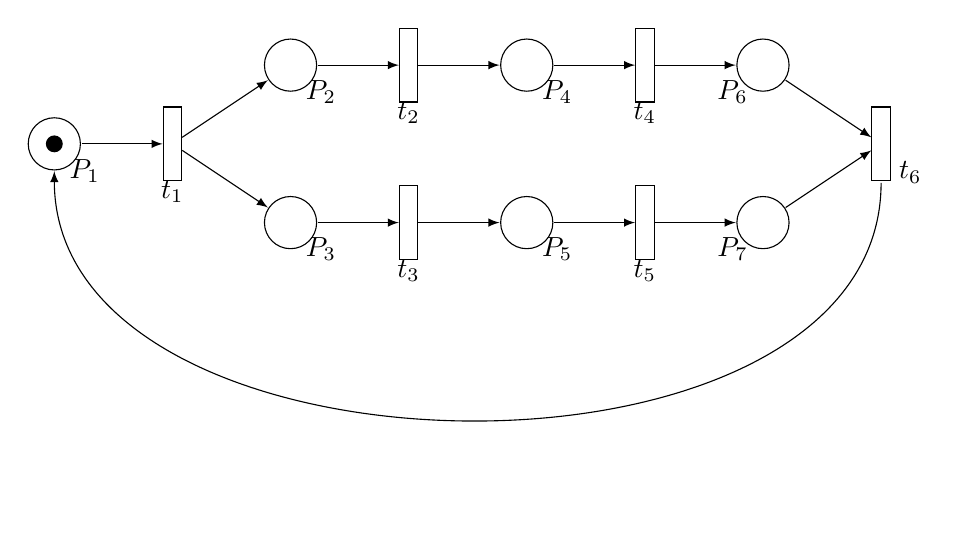
\begin{tikzpicture}
    % Liste des places
    \draw (-6,0) node[below right = 2pt] {$P_1$};
    \node[draw,circle,scale=2] (P1) at (-6, 0) {};
    \draw (-3,1) node[below right = 2pt] {$P_2$};
    \node[draw,circle,scale=2] (P2) at (-3, 1) {};
    \draw (-3,-1) node[below right = 2pt] {$P_3$};
    \node[draw,circle,scale=2] (P3) at (-3,-1) {};
    \draw (0,1) node[below right = 2pt] {$P_4$};
    \node[draw,circle,scale=2] (P4) at (0, 1) {};
    \draw (0,-1) node[below right = 2pt] {$P_5$};
    \node[draw,circle,scale=2] (P5) at (0,-1) {};
    \draw (3,1) node[below left = 2pt] {$P_6$};
    \node[draw,circle,scale=2] (P6) at (3, 1) {};
    \draw (3,-1) node[below left = 2pt] {$P_7$};
    \node[draw,circle,scale=2] (P7) at (3,-1) {};

    % Liste des transitions
    \draw (-4.5,0) node[below = 10pt] {$t_1$};
    \node[draw,rectangle,yscale=4] (t1) at (-4.5, 0) {};
    \draw (-1.5,-1) node[below = 10pt] {$t_3$};
    \node[draw,rectangle,yscale=4] (t3) at (-1.5, -1) {};
    \draw (-1.5,1) node[below = 10pt] {$t_2$};
    \node[draw,rectangle,yscale=4] (t2) at (-1.5, 1) {};
    \draw (1.5,-1) node[below = 10pt] {$t_5$};
    \node[draw,rectangle,yscale=4] (t5) at (1.5, -1) {};
    \draw (1.5,1) node[below = 10pt] {$t_4$};
    \node[draw,rectangle,yscale=4] (t4) at (1.5, 1) {};
    \draw (4.5,0) node[below right = 3pt] {$t_6$};
    \node[draw,rectangle,yscale=4] (t6) at (4.5, 0) {};

    % Liste des arcs
    \draw[->,>=latex] (P1) -- (t1);
    \draw[->,>=latex] (t1) -- (P2);
    \draw[->,>=latex] (t1) -- (P3);
    \draw[->,>=latex] (P3) -- (t3);
    \draw[->,>=latex] (P2) -- (t2);
    \draw[->,>=latex] (t2) -- (P4);
    \draw[->,>=latex] (t3) -- (P5);
    \draw[->,>=latex] (P4) -- (t4);
    \draw[->,>=latex] (P5) -- (t5);
    \draw[->,>=latex] (t4) -- (P6);
    \draw[->,>=latex] (t5) -- (P7);
    \draw[->,>=latex] (P6) -- (t6);
    \draw[->,>=latex] (P7) -- (t6);
    \draw[->,>=latex] (t6) to[out=-90,in=-90] (P1);

    % Marquage 
    \draw [fill](-6,0) circle (0.1) ;
  \end{tikzpicture}
  \caption{Réseau de petri associé au système d'impréssion par pochoir} \label{fig:M1}
\end{figure}

\subsection{Question 2}
Faisons tourner le système, à l'état initiale nous avons le réseau de la figure 1.\\
Lorsque la pièce est insérée dans le système et que les pochoirs sont prêt, le signal $p \wedge q$ est envoyé :

\begin{figure}[H]
  \centering
  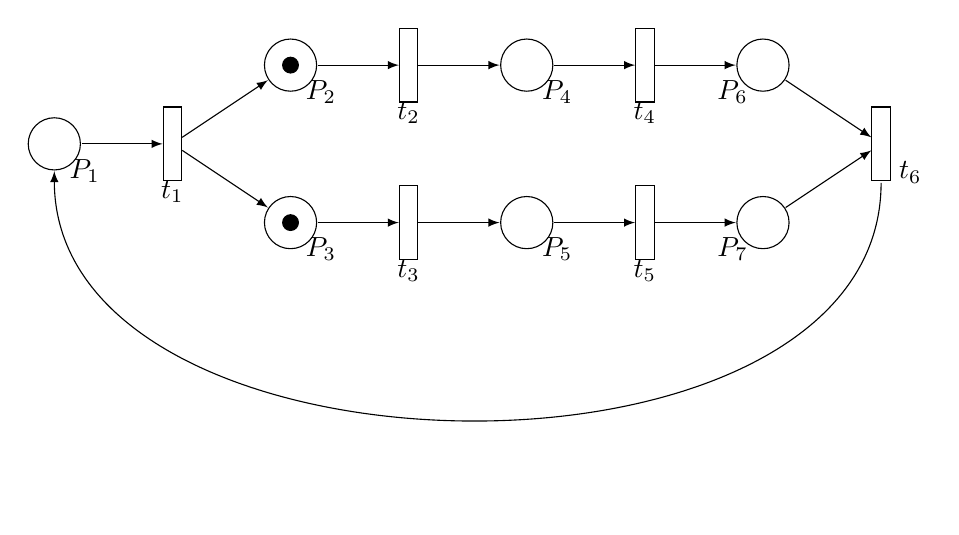
\begin{tikzpicture}
    % Liste des places
    \draw (-6,0) node[below right = 2pt] {$P_1$};
    \node[draw,circle,scale=2] (P1) at (-6, 0) {};
    \draw (-3,1) node[below right = 2pt] {$P_2$};
    \node[draw,circle,scale=2] (P2) at (-3, 1) {};
    \draw (-3,-1) node[below right = 2pt] {$P_3$};
    \node[draw,circle,scale=2] (P3) at (-3,-1) {};
    \draw (0,1) node[below right = 2pt] {$P_4$};
    \node[draw,circle,scale=2] (P4) at (0, 1) {};
    \draw (0,-1) node[below right = 2pt] {$P_5$};
    \node[draw,circle,scale=2] (P5) at (0,-1) {};
    \draw (3,1) node[below left = 2pt] {$P_6$};
    \node[draw,circle,scale=2] (P6) at (3, 1) {};
    \draw (3,-1) node[below left = 2pt] {$P_7$};
    \node[draw,circle,scale=2] (P7) at (3,-1) {};

    % Liste des transitions
    \draw (-4.5,0) node[below = 10pt] {$t_1$};
    \node[draw,rectangle,yscale=4] (t1) at (-4.5, 0) {};
    \draw (-1.5,-1) node[below = 10pt] {$t_3$};
    \node[draw,rectangle,yscale=4] (t3) at (-1.5, -1) {};
    \draw (-1.5,1) node[below = 10pt] {$t_2$};
    \node[draw,rectangle,yscale=4] (t2) at (-1.5, 1) {};
    \draw (1.5,-1) node[below = 10pt] {$t_5$};
    \node[draw,rectangle,yscale=4] (t5) at (1.5, -1) {};
    \draw (1.5,1) node[below = 10pt] {$t_4$};
    \node[draw,rectangle,yscale=4] (t4) at (1.5, 1) {};
    \draw (4.5,0) node[below right= 3pt] {$t_6$};
    \node[draw,rectangle,yscale=4] (t6) at (4.5, 0) {};

    % Liste des arcs
    \draw[->,>=latex] (P1) -- (t1);
    \draw[->,>=latex] (t1) -- (P2);
    \draw[->,>=latex] (t1) -- (P3);
    \draw[->,>=latex] (P3) -- (t3);
    \draw[->,>=latex] (P2) -- (t2);
    \draw[->,>=latex] (t2) -- (P4);
    \draw[->,>=latex] (t3) -- (P5);
    \draw[->,>=latex] (P4) -- (t4);
    \draw[->,>=latex] (P5) -- (t5);
    \draw[->,>=latex] (t4) -- (P6);
    \draw[->,>=latex] (t5) -- (P7);
    \draw[->,>=latex] (P6) -- (t6);
    \draw[->,>=latex] (P7) -- (t6);
    \draw[->,>=latex] (t6) to[out=-90,in=-90] (P1);

    % Marquage 
    \draw [fill](-3,1) circle (0.1) ;
    \draw [fill](-3,-1) circle (0.1) ;
  \end{tikzpicture}
  \caption{Réseau après initialisation du système} \label{fig:M2}
\end{figure}

\newpage

On peut ensuite faire avancer le pochoir droit (fig. 3) ou gauche (fig.4) :

\begin{figure}[H]
  \centering
  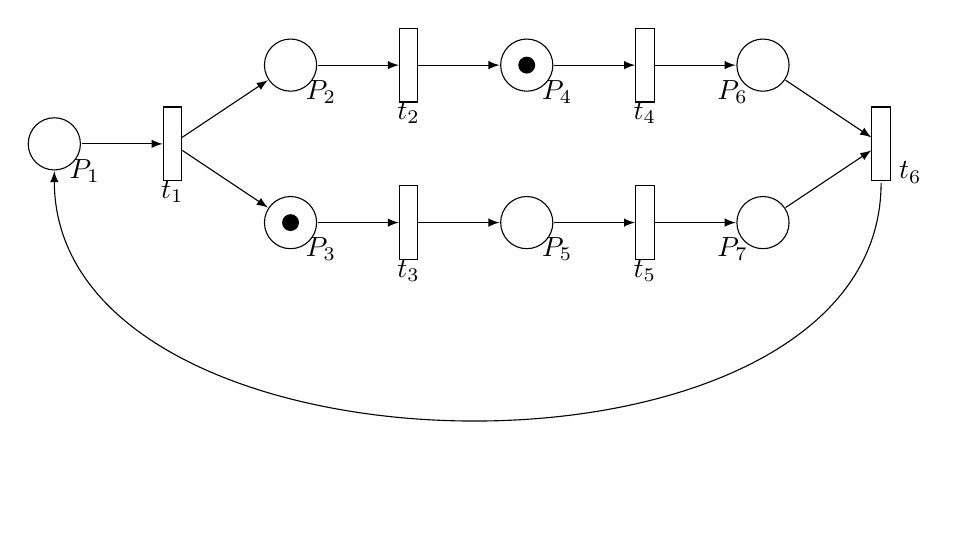
\begin{tikzpicture}
    % Liste des places
    \draw (-6,0) node[below right = 2pt] {$P_1$};
    \node[draw,circle,scale=2] (P1) at (-6, 0) {};
    \draw (-3,1) node[below right = 2pt] {$P_2$};
    \node[draw,circle,scale=2] (P2) at (-3, 1) {};
    \draw (-3,-1) node[below right = 2pt] {$P_3$};
    \node[draw,circle,scale=2] (P3) at (-3,-1) {};
    \draw (0,1) node[below right = 2pt] {$P_4$};
    \node[draw,circle,scale=2] (P4) at (0, 1) {};
    \draw (0,-1) node[below right = 2pt] {$P_5$};
    \node[draw,circle,scale=2] (P5) at (0,-1) {};
    \draw (3,1) node[below left = 2pt] {$P_6$};
    \node[draw,circle,scale=2] (P6) at (3, 1) {};
    \draw (3,-1) node[below left = 2pt] {$P_7$};
    \node[draw,circle,scale=2] (P7) at (3,-1) {};

    % Liste des transitions
    \draw (-4.5,0) node[below = 10pt] {$t_1$};
    \node[draw,rectangle,yscale=4] (t1) at (-4.5, 0) {};
    \draw (-1.5,-1) node[below = 10pt] {$t_3$};
    \node[draw,rectangle,yscale=4] (t3) at (-1.5, -1) {};
    \draw (-1.5,1) node[below = 10pt] {$t_2$};
    \node[draw,rectangle,yscale=4] (t2) at (-1.5, 1) {};
    \draw (1.5,-1) node[below = 10pt] {$t_5$};
    \node[draw,rectangle,yscale=4] (t5) at (1.5, -1) {};
    \draw (1.5,1) node[below = 10pt] {$t_4$};
    \node[draw,rectangle,yscale=4] (t4) at (1.5, 1) {};
    \draw (4.5,0) node[below right= 3pt] {$t_6$};
    \node[draw,rectangle,yscale=4] (t6) at (4.5, 0) {};

    % Liste des arcs
    \draw[->,>=latex] (P1) -- (t1);
    \draw[->,>=latex] (t1) -- (P2);
    \draw[->,>=latex] (t1) -- (P3);
    \draw[->,>=latex] (P3) -- (t3);
    \draw[->,>=latex] (P2) -- (t2);
    \draw[->,>=latex] (t2) -- (P4);
    \draw[->,>=latex] (t3) -- (P5);
    \draw[->,>=latex] (P4) -- (t4);
    \draw[->,>=latex] (P5) -- (t5);
    \draw[->,>=latex] (t4) -- (P6);
    \draw[->,>=latex] (t5) -- (P7);
    \draw[->,>=latex] (P6) -- (t6);
    \draw[->,>=latex] (P7) -- (t6);
    \draw[->,>=latex] (t6) to[out=-90,in=-90] (P1);

    % Marquage 
    \draw [fill](0,1) circle (0.1) ;
    \draw [fill](-3,-1) circle (0.1) ;
  \end{tikzpicture}
  \caption{Réseau après l'avancement du pochoir droit} \label{fig:M3}
\end{figure}

\begin{figure}[H]
  \centering
  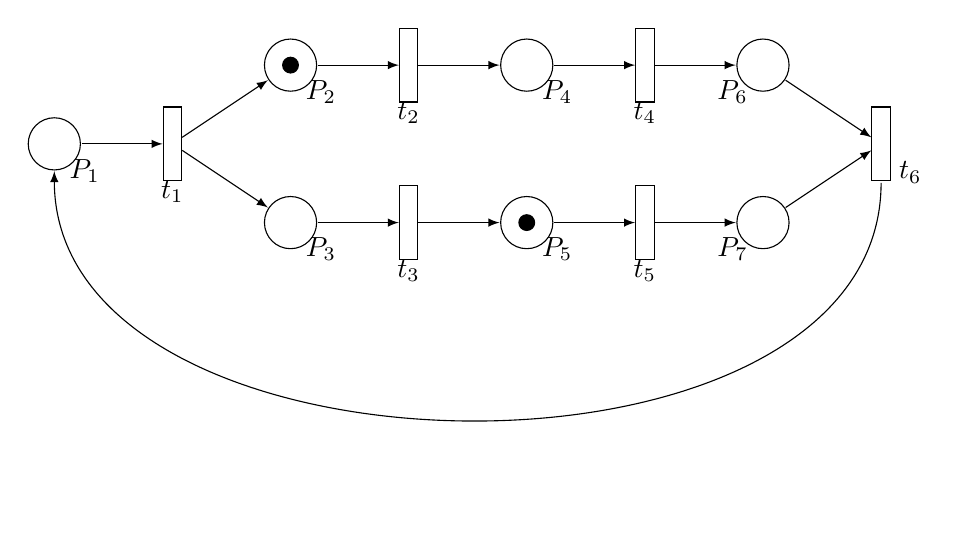
\begin{tikzpicture}
    % Liste des places
    \draw (-6,0) node[below right = 2pt] {$P_1$};
    \node[draw,circle,scale=2] (P1) at (-6, 0) {};
    \draw (-3,1) node[below right = 2pt] {$P_2$};
    \node[draw,circle,scale=2] (P2) at (-3, 1) {};
    \draw (-3,-1) node[below right = 2pt] {$P_3$};
    \node[draw,circle,scale=2] (P3) at (-3,-1) {};
    \draw (0,1) node[below right = 2pt] {$P_4$};
    \node[draw,circle,scale=2] (P4) at (0, 1) {};
    \draw (0,-1) node[below right = 2pt] {$P_5$};
    \node[draw,circle,scale=2] (P5) at (0,-1) {};
    \draw (3,1) node[below left = 2pt] {$P_6$};
    \node[draw,circle,scale=2] (P6) at (3, 1) {};
    \draw (3,-1) node[below left = 2pt] {$P_7$};
    \node[draw,circle,scale=2] (P7) at (3,-1) {};

    % Liste des transitions
    \draw (-4.5,0) node[below = 10pt] {$t_1$};
    \node[draw,rectangle,yscale=4] (t1) at (-4.5, 0) {};
    \draw (-1.5,-1) node[below = 10pt] {$t_3$};
    \node[draw,rectangle,yscale=4] (t3) at (-1.5, -1) {};
    \draw (-1.5,1) node[below = 10pt] {$t_2$};
    \node[draw,rectangle,yscale=4] (t2) at (-1.5, 1) {};
    \draw (1.5,-1) node[below = 10pt] {$t_5$};
    \node[draw,rectangle,yscale=4] (t5) at (1.5, -1) {};
    \draw (1.5,1) node[below = 10pt] {$t_4$};
    \node[draw,rectangle,yscale=4] (t4) at (1.5, 1) {};
    \draw (4.5,0) node[below right= 3pt] {$t_6$};
    \node[draw,rectangle,yscale=4] (t6) at (4.5, 0) {};

    % Liste des arcs
    \draw[->,>=latex] (P1) -- (t1);
    \draw[->,>=latex] (t1) -- (P2);
    \draw[->,>=latex] (t1) -- (P3);
    \draw[->,>=latex] (P3) -- (t3);
    \draw[->,>=latex] (P2) -- (t2);
    \draw[->,>=latex] (t2) -- (P4);
    \draw[->,>=latex] (t3) -- (P5);
    \draw[->,>=latex] (P4) -- (t4);
    \draw[->,>=latex] (P5) -- (t5);
    \draw[->,>=latex] (t4) -- (P6);
    \draw[->,>=latex] (t5) -- (P7);
    \draw[->,>=latex] (P6) -- (t6);
    \draw[->,>=latex] (P7) -- (t6);
    \draw[->,>=latex] (t6) to[out=-90,in=-90] (P1);

    % Marquage 
    \draw [fill](-3,1) circle (0.1) ;
    \draw [fill](0,-1) circle (0.1) ;
  \end{tikzpicture}
  \caption{Réseau après l'avancement du pochoir gauche} \label{fig:M4}
\end{figure}

A cet instant, on a plusieurs évolution du système possible : 
\begin{enumerate}
  \item Si le pochoir droit a été avancé : \\
    \begin{itemize}
      \item On peut alors le reculer : fig. 7
      \item On peut avancer le pochoir gauche : fig. 5
    \end{itemize}
  \item Si le pochoir gauche a été avancé : \\
    \begin{itemize}
      \item On peut alors le reculer : fig. 6
      \item On peut avancer le pochoir droit : fig. 5
    \end{itemize}
\end{enumerate}

\begin{figure}[H]
  \centering
  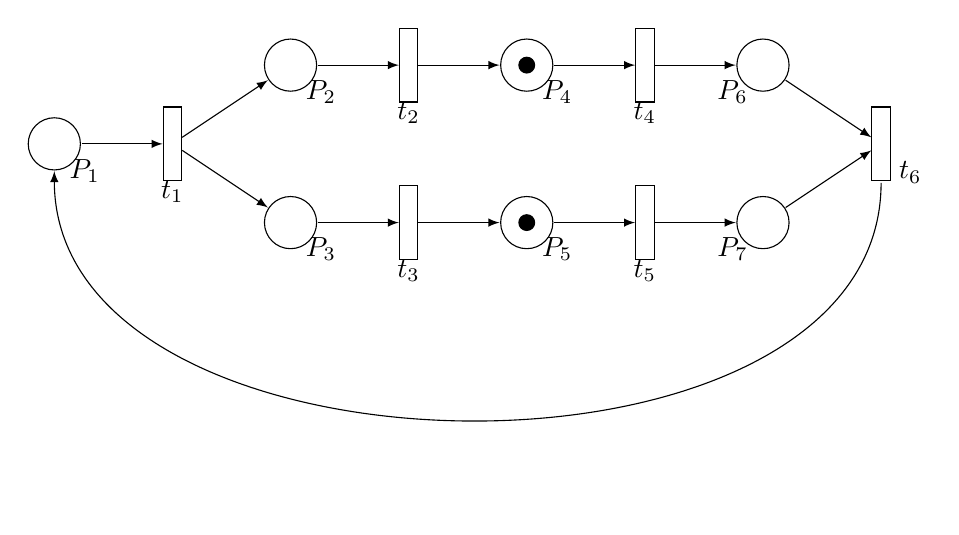
\begin{tikzpicture}
    % Liste des places
    \draw (-6,0) node[below right = 2pt] {$P_1$};
    \node[draw,circle,scale=2] (P1) at (-6, 0) {};
    \draw (-3,1) node[below right = 2pt] {$P_2$};
    \node[draw,circle,scale=2] (P2) at (-3, 1) {};
    \draw (-3,-1) node[below right = 2pt] {$P_3$};
    \node[draw,circle,scale=2] (P3) at (-3,-1) {};
    \draw (0,1) node[below right = 2pt] {$P_4$};
    \node[draw,circle,scale=2] (P4) at (0, 1) {};
    \draw (0,-1) node[below right = 2pt] {$P_5$};
    \node[draw,circle,scale=2] (P5) at (0,-1) {};
    \draw (3,1) node[below left = 2pt] {$P_6$};
    \node[draw,circle,scale=2] (P6) at (3, 1) {};
    \draw (3,-1) node[below left = 2pt] {$P_7$};
    \node[draw,circle,scale=2] (P7) at (3,-1) {};

    % Liste des transitions
    \draw (-4.5,0) node[below = 10pt] {$t_1$};
    \node[draw,rectangle,yscale=4] (t1) at (-4.5, 0) {};
    \draw (-1.5,-1) node[below = 10pt] {$t_3$};
    \node[draw,rectangle,yscale=4] (t3) at (-1.5, -1) {};
    \draw (-1.5,1) node[below = 10pt] {$t_2$};
    \node[draw,rectangle,yscale=4] (t2) at (-1.5, 1) {};
    \draw (1.5,-1) node[below = 10pt] {$t_5$};
    \node[draw,rectangle,yscale=4] (t5) at (1.5, -1) {};
    \draw (1.5,1) node[below = 10pt] {$t_4$};
    \node[draw,rectangle,yscale=4] (t4) at (1.5, 1) {};
    \draw (4.5,0) node[below right= 3pt] {$t_6$};
    \node[draw,rectangle,yscale=4] (t6) at (4.5, 0) {};

    % Liste des arcs
    \draw[->,>=latex] (P1) -- (t1);
    \draw[->,>=latex] (t1) -- (P2);
    \draw[->,>=latex] (t1) -- (P3);
    \draw[->,>=latex] (P3) -- (t3);
    \draw[->,>=latex] (P2) -- (t2);
    \draw[->,>=latex] (t2) -- (P4);
    \draw[->,>=latex] (t3) -- (P5);
    \draw[->,>=latex] (P4) -- (t4);
    \draw[->,>=latex] (P5) -- (t5);
    \draw[->,>=latex] (t4) -- (P6);
    \draw[->,>=latex] (t5) -- (P7);
    \draw[->,>=latex] (P6) -- (t6);
    \draw[->,>=latex] (P7) -- (t6);
    \draw[->,>=latex] (t6) to[out=-90,in=-90] (P1);

    % Marquage 
    \draw [fill](0,1) circle (0.1) ;
    \draw [fill](0,-1) circle (0.1) ;
  \end{tikzpicture}
  \caption{Réseau après l'avancement du pochoir gauche et droit} \label{fig:M5}
\end{figure}

\begin{figure}[H]
  \centering
  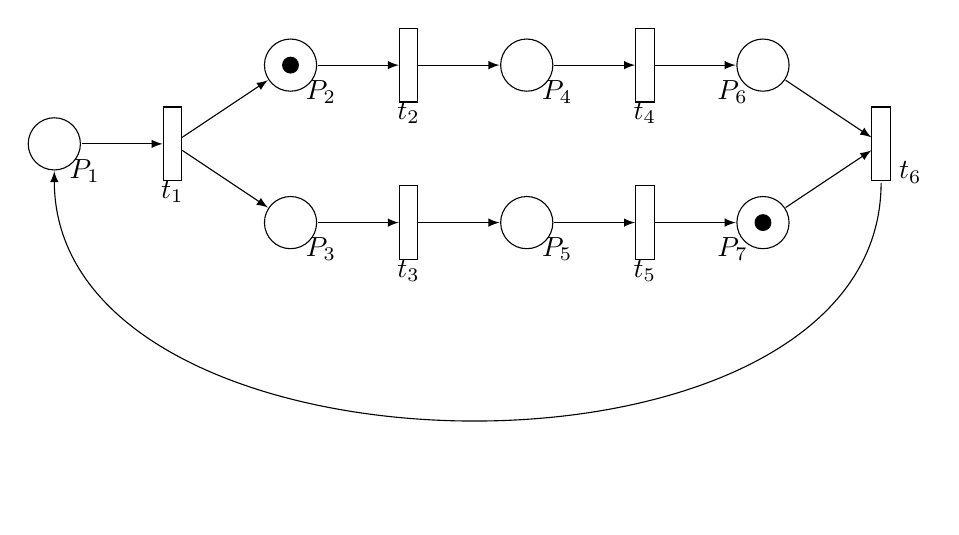
\begin{tikzpicture}
    % Liste des places
    \draw (-6,0) node[below right = 2pt] {$P_1$};
    \node[draw,circle,scale=2] (P1) at (-6, 0) {};
    \draw (-3,1) node[below right = 2pt] {$P_2$};
    \node[draw,circle,scale=2] (P2) at (-3, 1) {};
    \draw (-3,-1) node[below right = 2pt] {$P_3$};
    \node[draw,circle,scale=2] (P3) at (-3,-1) {};
    \draw (0,1) node[below right = 2pt] {$P_4$};
    \node[draw,circle,scale=2] (P4) at (0, 1) {};
    \draw (0,-1) node[below right = 2pt] {$P_5$};
    \node[draw,circle,scale=2] (P5) at (0,-1) {};
    \draw (3,1) node[below left = 2pt] {$P_6$};
    \node[draw,circle,scale=2] (P6) at (3, 1) {};
    \draw (3,-1) node[below left = 2pt] {$P_7$};
    \node[draw,circle,scale=2] (P7) at (3,-1) {};

    % Liste des transitions
    \draw (-4.5,0) node[below = 10pt] {$t_1$};
    \node[draw,rectangle,yscale=4] (t1) at (-4.5, 0) {};
    \draw (-1.5,-1) node[below = 10pt] {$t_3$};
    \node[draw,rectangle,yscale=4] (t3) at (-1.5, -1) {};
    \draw (-1.5,1) node[below = 10pt] {$t_2$};
    \node[draw,rectangle,yscale=4] (t2) at (-1.5, 1) {};
    \draw (1.5,-1) node[below = 10pt] {$t_5$};
    \node[draw,rectangle,yscale=4] (t5) at (1.5, -1) {};
    \draw (1.5,1) node[below = 10pt] {$t_4$};
    \node[draw,rectangle,yscale=4] (t4) at (1.5, 1) {};
    \draw (4.5,0) node[below right= 3pt] {$t_6$};
    \node[draw,rectangle,yscale=4] (t6) at (4.5, 0) {};

    % Liste des arcs
    \draw[->,>=latex] (P1) -- (t1);
    \draw[->,>=latex] (t1) -- (P2);
    \draw[->,>=latex] (t1) -- (P3);
    \draw[->,>=latex] (P3) -- (t3);
    \draw[->,>=latex] (P2) -- (t2);
    \draw[->,>=latex] (t2) -- (P4);
    \draw[->,>=latex] (t3) -- (P5);
    \draw[->,>=latex] (P4) -- (t4);
    \draw[->,>=latex] (P5) -- (t5);
    \draw[->,>=latex] (t4) -- (P6);
    \draw[->,>=latex] (t5) -- (P7);
    \draw[->,>=latex] (P6) -- (t6);
    \draw[->,>=latex] (P7) -- (t6);
    \draw[->,>=latex] (t6) to[out=-90,in=-90] (P1);

    % Marquage 
    \draw [fill](-3,1) circle (0.1) ;
    \draw [fill](3,-1) circle (0.1) ;
  \end{tikzpicture}
  \caption{Réseau après l'avancement et retour du pochoir gauche} \label{fig:M6}
\end{figure}

\begin{figure}[H]
  \centering
  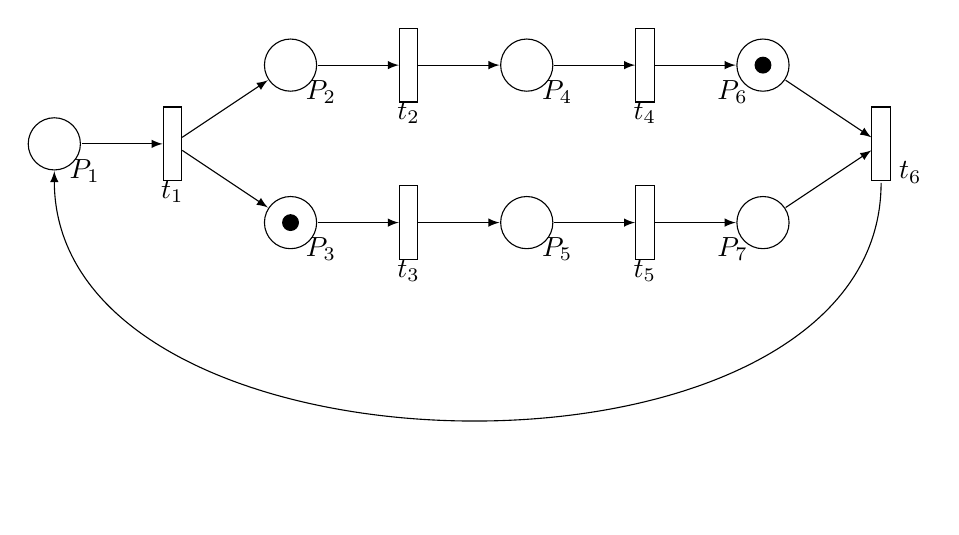
\begin{tikzpicture}
    % Liste des places
    \draw (-6,0) node[below right = 2pt] {$P_1$};
    \node[draw,circle,scale=2] (P1) at (-6, 0) {};
    \draw (-3,1) node[below right = 2pt] {$P_2$};
    \node[draw,circle,scale=2] (P2) at (-3, 1) {};
    \draw (-3,-1) node[below right = 2pt] {$P_3$};
    \node[draw,circle,scale=2] (P3) at (-3,-1) {};
    \draw (0,1) node[below right = 2pt] {$P_4$};
    \node[draw,circle,scale=2] (P4) at (0, 1) {};
    \draw (0,-1) node[below right = 2pt] {$P_5$};
    \node[draw,circle,scale=2] (P5) at (0,-1) {};
    \draw (3,1) node[below left = 2pt] {$P_6$};
    \node[draw,circle,scale=2] (P6) at (3, 1) {};
    \draw (3,-1) node[below left = 2pt] {$P_7$};
    \node[draw,circle,scale=2] (P7) at (3,-1) {};

    % Liste des transitions
    \draw (-4.5,0) node[below = 10pt] {$t_1$};
    \node[draw,rectangle,yscale=4] (t1) at (-4.5, 0) {};
    \draw (-1.5,-1) node[below = 10pt] {$t_3$};
    \node[draw,rectangle,yscale=4] (t3) at (-1.5, -1) {};
    \draw (-1.5,1) node[below = 10pt] {$t_2$};
    \node[draw,rectangle,yscale=4] (t2) at (-1.5, 1) {};
    \draw (1.5,-1) node[below = 10pt] {$t_5$};
    \node[draw,rectangle,yscale=4] (t5) at (1.5, -1) {};
    \draw (1.5,1) node[below = 10pt] {$t_4$};
    \node[draw,rectangle,yscale=4] (t4) at (1.5, 1) {};
    \draw (4.5,0) node[below right= 3pt] {$t_6$};
    \node[draw,rectangle,yscale=4] (t6) at (4.5, 0) {};

    % Liste des arcs
    \draw[->,>=latex] (P1) -- (t1);
    \draw[->,>=latex] (t1) -- (P2);
    \draw[->,>=latex] (t1) -- (P3);
    \draw[->,>=latex] (P3) -- (t3);
    \draw[->,>=latex] (P2) -- (t2);
    \draw[->,>=latex] (t2) -- (P4);
    \draw[->,>=latex] (t3) -- (P5);
    \draw[->,>=latex] (P4) -- (t4);
    \draw[->,>=latex] (P5) -- (t5);
    \draw[->,>=latex] (t4) -- (P6);
    \draw[->,>=latex] (t5) -- (P7);
    \draw[->,>=latex] (P6) -- (t6);
    \draw[->,>=latex] (P7) -- (t6);
    \draw[->,>=latex] (t6) to[out=-90,in=-90] (P1);

    % Marquage 
    \draw [fill](3,1) circle (0.1) ;
    \draw [fill](-3,-1) circle (0.1) ;
  \end{tikzpicture}
  \caption{Réseau après l'avancement et le retour du pochoir droit} \label{fig:M7}
\end{figure}

On obtient ainsi de plus en plus de cas à étudier :\\
\begin{enumerate}
  \item Si on a fait avancer et reculer le pochoir droit
    \begin{itemize}
      \item On doit alors faire avancer le pochoir gauche : fig. 9
    \end{itemize}
  \item Si on a fait avancer et reculer le pochoir gauche
    \begin{itemize}
      \item On doit alors faire avancer le pochoir droit : fig. 8
    \end{itemize}
  \item Si on a fait avancer les deux pochoirs
    \begin{itemize}
      \item On doit alors faire reculer l'un des deux pochoirs
        \begin{itemize}
          \item pochoir droit : fig. 9
          \item pochoir gauche : fig. 8
        \end{itemize}
   \end{itemize}
\end{enumerate}


\begin{figure}[H]
  \centering
  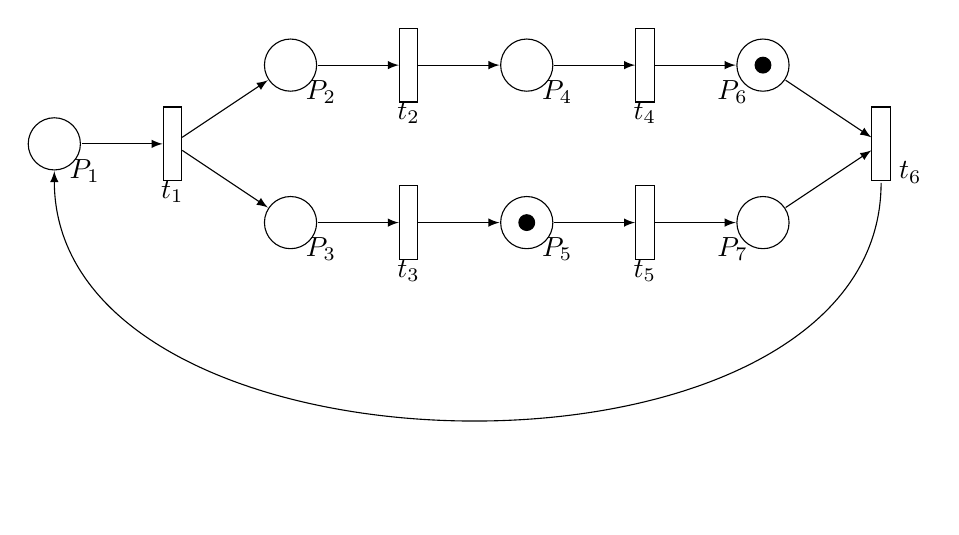
\begin{tikzpicture}
    % Liste des places
    \draw (-6,0) node[below right = 2pt] {$P_1$};
    \node[draw,circle,scale=2] (P1) at (-6, 0) {};
    \draw (-3,1) node[below right = 2pt] {$P_2$};
    \node[draw,circle,scale=2] (P2) at (-3, 1) {};
    \draw (-3,-1) node[below right = 2pt] {$P_3$};
    \node[draw,circle,scale=2] (P3) at (-3,-1) {};
    \draw (0,1) node[below right = 2pt] {$P_4$};
    \node[draw,circle,scale=2] (P4) at (0, 1) {};
    \draw (0,-1) node[below right = 2pt] {$P_5$};
    \node[draw,circle,scale=2] (P5) at (0,-1) {};
    \draw (3,1) node[below left = 2pt] {$P_6$};
    \node[draw,circle,scale=2] (P6) at (3, 1) {};
    \draw (3,-1) node[below left = 2pt] {$P_7$};
    \node[draw,circle,scale=2] (P7) at (3,-1) {};

    % Liste des transitions
    \draw (-4.5,0) node[below = 10pt] {$t_1$};
    \node[draw,rectangle,yscale=4] (t1) at (-4.5, 0) {};
    \draw (-1.5,-1) node[below = 10pt] {$t_3$};
    \node[draw,rectangle,yscale=4] (t3) at (-1.5, -1) {};
    \draw (-1.5,1) node[below = 10pt] {$t_2$};
    \node[draw,rectangle,yscale=4] (t2) at (-1.5, 1) {};
    \draw (1.5,-1) node[below = 10pt] {$t_5$};
    \node[draw,rectangle,yscale=4] (t5) at (1.5, -1) {};
    \draw (1.5,1) node[below = 10pt] {$t_4$};
    \node[draw,rectangle,yscale=4] (t4) at (1.5, 1) {};
    \draw (4.5,0) node[below right= 3pt] {$t_6$};
    \node[draw,rectangle,yscale=4] (t6) at (4.5, 0) {};

    % Liste des arcs
    \draw[->,>=latex] (P1) -- (t1);
    \draw[->,>=latex] (t1) -- (P2);
    \draw[->,>=latex] (t1) -- (P3);
    \draw[->,>=latex] (P3) -- (t3);
    \draw[->,>=latex] (P2) -- (t2);
    \draw[->,>=latex] (t2) -- (P4);
    \draw[->,>=latex] (t3) -- (P5);
    \draw[->,>=latex] (P4) -- (t4);
    \draw[->,>=latex] (P5) -- (t5);
    \draw[->,>=latex] (t4) -- (P6);
    \draw[->,>=latex] (t5) -- (P7);
    \draw[->,>=latex] (P6) -- (t6);
    \draw[->,>=latex] (P7) -- (t6);
    \draw[->,>=latex] (t6) to[out=-90,in=-90] (P1);

    % Marquage 
    \draw [fill](3,1) circle (0.1) ;
    \draw [fill](0,-1) circle (0.1) ;
  \end{tikzpicture}
  \caption{Réseau après l'avancement des 2 pochoirs et le retour du pochoir droit} \label{fig:M8}
\end{figure}

\begin{figure}[H]
  \centering
  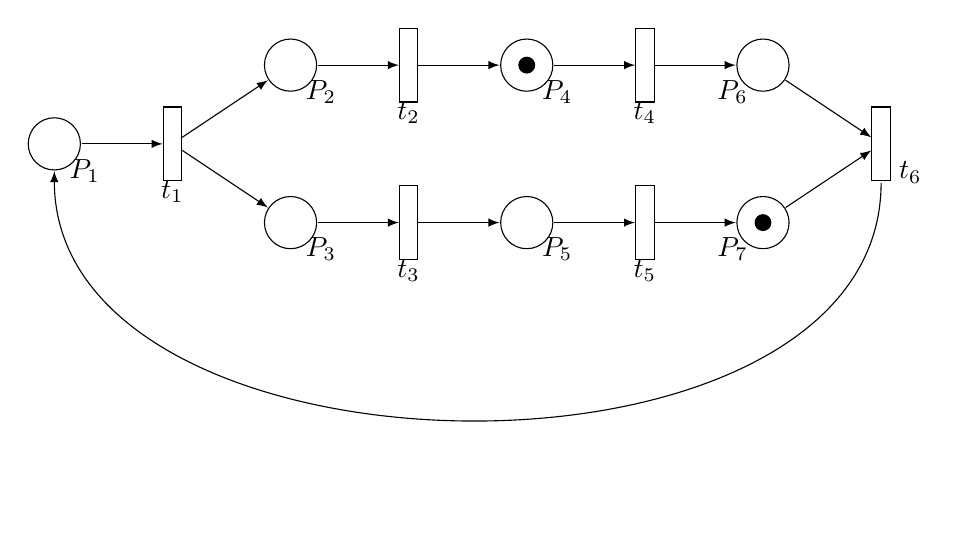
\begin{tikzpicture}
    % Liste des places
    \draw (-6,0) node[below right = 2pt] {$P_1$};
    \node[draw,circle,scale=2] (P1) at (-6, 0) {};
    \draw (-3,1) node[below right = 2pt] {$P_2$};
    \node[draw,circle,scale=2] (P2) at (-3, 1) {};
    \draw (-3,-1) node[below right = 2pt] {$P_3$};
    \node[draw,circle,scale=2] (P3) at (-3,-1) {};
    \draw (0,1) node[below right = 2pt] {$P_4$};
    \node[draw,circle,scale=2] (P4) at (0, 1) {};
    \draw (0,-1) node[below right = 2pt] {$P_5$};
    \node[draw,circle,scale=2] (P5) at (0,-1) {};
    \draw (3,1) node[below left = 2pt] {$P_6$};
    \node[draw,circle,scale=2] (P6) at (3, 1) {};
    \draw (3,-1) node[below left = 2pt] {$P_7$};
    \node[draw,circle,scale=2] (P7) at (3,-1) {};

    % Liste des transitions
    \draw (-4.5,0) node[below = 10pt] {$t_1$};
    \node[draw,rectangle,yscale=4] (t1) at (-4.5, 0) {};
    \draw (-1.5,-1) node[below = 10pt] {$t_3$};
    \node[draw,rectangle,yscale=4] (t3) at (-1.5, -1) {};
    \draw (-1.5,1) node[below = 10pt] {$t_2$};
    \node[draw,rectangle,yscale=4] (t2) at (-1.5, 1) {};
    \draw (1.5,-1) node[below = 10pt] {$t_5$};
    \node[draw,rectangle,yscale=4] (t5) at (1.5, -1) {};
    \draw (1.5,1) node[below = 10pt] {$t_4$};
    \node[draw,rectangle,yscale=4] (t4) at (1.5, 1) {};
    \draw (4.5,0) node[below right= 3pt] {$t_6$};
    \node[draw,rectangle,yscale=4] (t6) at (4.5, 0) {};

    % Liste des arcs
    \draw[->,>=latex] (P1) -- (t1);
    \draw[->,>=latex] (t1) -- (P2);
    \draw[->,>=latex] (t1) -- (P3);
    \draw[->,>=latex] (P3) -- (t3);
    \draw[->,>=latex] (P2) -- (t2);
    \draw[->,>=latex] (t2) -- (P4);
    \draw[->,>=latex] (t3) -- (P5);
    \draw[->,>=latex] (P4) -- (t4);
    \draw[->,>=latex] (P5) -- (t5);
    \draw[->,>=latex] (t4) -- (P6);
    \draw[->,>=latex] (t5) -- (P7);
    \draw[->,>=latex] (P6) -- (t6);
    \draw[->,>=latex] (P7) -- (t6);
    \draw[->,>=latex] (t6) to[out=-90,in=-90] (P1);

    % Marquage 
    \draw [fill](0,1) circle (0.1) ;
    \draw [fill](3,-1) circle (0.1) ;
  \end{tikzpicture}
  \caption{Réseau après l'avancement des 2 pochoirs et le retour du pochoir gauche} \label{fig:M9}
\end{figure}

Dans les deux cas ci-dessus, il nous reste à faire reculer le pochoir qui ne l'a pas encore fait.
Et on obtient le même réseau dans les 2 cas :

\begin{figure}[H]
  \centering
  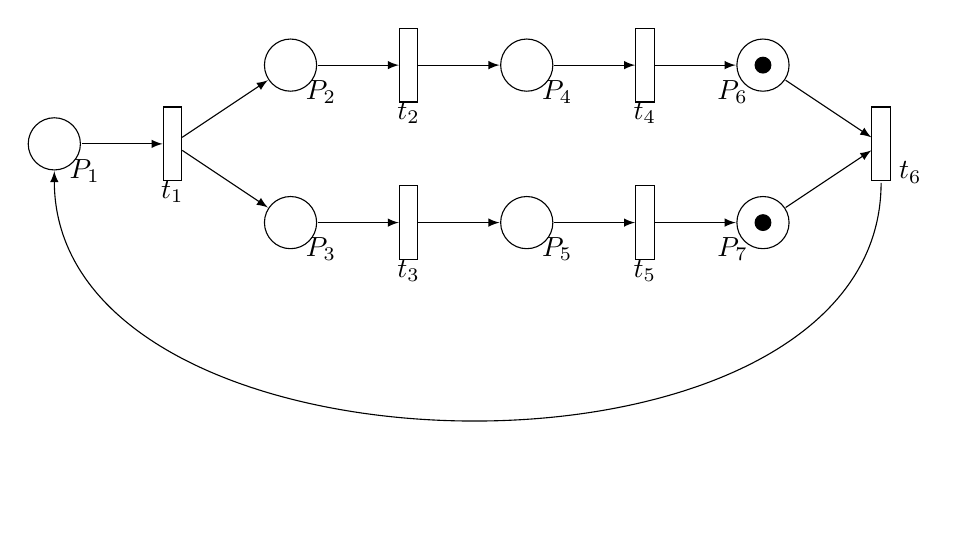
\begin{tikzpicture}
    % Liste des places
    \draw (-6,0) node[below right = 2pt] {$P_1$};
    \node[draw,circle,scale=2] (P1) at (-6, 0) {};
    \draw (-3,1) node[below right = 2pt] {$P_2$};
    \node[draw,circle,scale=2] (P2) at (-3, 1) {};
    \draw (-3,-1) node[below right = 2pt] {$P_3$};
    \node[draw,circle,scale=2] (P3) at (-3,-1) {};
    \draw (0,1) node[below right = 2pt] {$P_4$};
    \node[draw,circle,scale=2] (P4) at (0, 1) {};
    \draw (0,-1) node[below right = 2pt] {$P_5$};
    \node[draw,circle,scale=2] (P5) at (0,-1) {};
    \draw (3,1) node[below left = 2pt] {$P_6$};
    \node[draw,circle,scale=2] (P6) at (3, 1) {};
    \draw (3,-1) node[below left = 2pt] {$P_7$};
    \node[draw,circle,scale=2] (P7) at (3,-1) {};

    % Liste des transitions
    \draw (-4.5,0) node[below = 10pt] {$t_1$};
    \node[draw,rectangle,yscale=4] (t1) at (-4.5, 0) {};
    \draw (-1.5,-1) node[below = 10pt] {$t_3$};
    \node[draw,rectangle,yscale=4] (t3) at (-1.5, -1) {};
    \draw (-1.5,1) node[below = 10pt] {$t_2$};
    \node[draw,rectangle,yscale=4] (t2) at (-1.5, 1) {};
    \draw (1.5,-1) node[below = 10pt] {$t_5$};
    \node[draw,rectangle,yscale=4] (t5) at (1.5, -1) {};
    \draw (1.5,1) node[below = 10pt] {$t_4$};
    \node[draw,rectangle,yscale=4] (t4) at (1.5, 1) {};
    \draw (4.5,0) node[below right= 3pt] {$t_6$};
    \node[draw,rectangle,yscale=4] (t6) at (4.5, 0) {};

    % Liste des arcs
    \draw[->,>=latex] (P1) -- (t1);
    \draw[->,>=latex] (t1) -- (P2);
    \draw[->,>=latex] (t1) -- (P3);
    \draw[->,>=latex] (P3) -- (t3);
    \draw[->,>=latex] (P2) -- (t2);
    \draw[->,>=latex] (t2) -- (P4);
    \draw[->,>=latex] (t3) -- (P5);
    \draw[->,>=latex] (P4) -- (t4);
    \draw[->,>=latex] (P5) -- (t5);
    \draw[->,>=latex] (t4) -- (P6);
    \draw[->,>=latex] (t5) -- (P7);
    \draw[->,>=latex] (P6) -- (t6);
    \draw[->,>=latex] (P7) -- (t6);
    \draw[->,>=latex] (t6) to[out=-90,in=-90] (P1);

    % Marquage 
    \draw [fill](3,1) circle (0.1) ;
    \draw [fill](3,-1) circle (0.1) ;
  \end{tikzpicture}
  \caption{Réseau après l'avancement et le retour des 2 pochoirs} \label{fig:M10}
\end{figure}

Enfin, la piece est imprimée et le système revient à son état initiale en fig 1.

\subsection{Question 3}
Comme nous l'avons, vu en faisant évoluer le système et le reseau, chaque place ne peut recevoir qu'un jeton avec le marquage initiale $M0 = (1,0,0,0,0,0,0)$.\\
Le reseau est donc cohérent.

\subsection{Question 4}
Les signaux incompatibles, tel que $Ad \wedge \overline{Rd}$ et $\overline{Ad} \wedge Rd$, se trouve tous la même ligne du reseau, où un seul jeton navigue.
Donc si l'une de ces places possède un jeton les autres ne peuvent pas en avoir un.
Ainsi, il y a bien une exclusion mutuelle entre ces places.

\subsection{Question 5}

Nous pouvons construire le graphe de marquage suivant :

\begin{figure}[H]
  \centering
  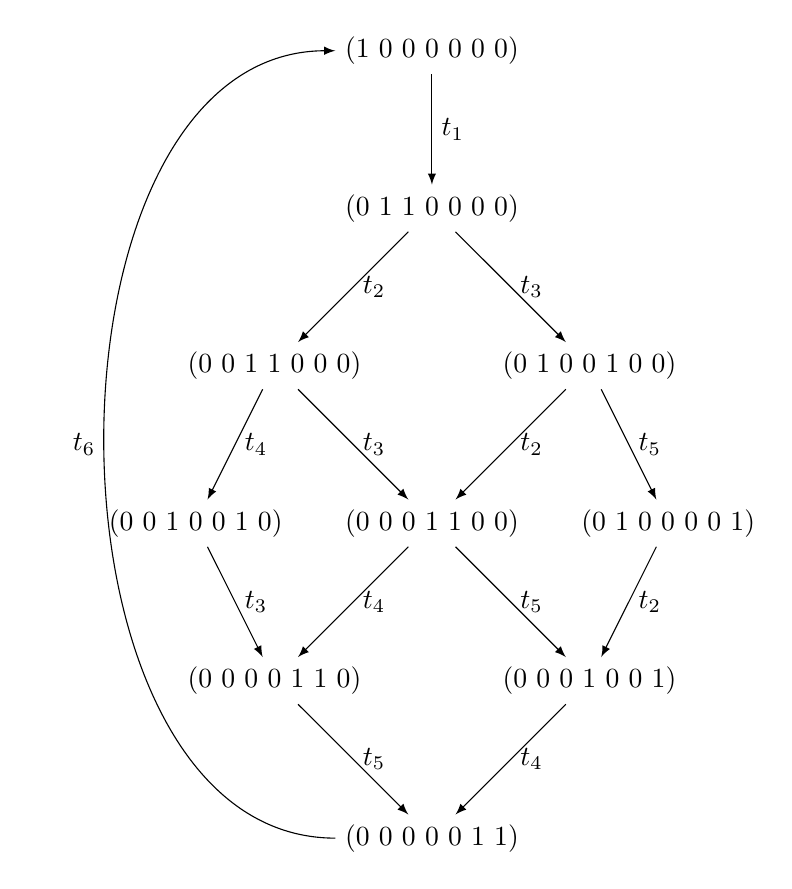
\begin{tikzpicture}
    % Liste des Marquage
    \node (M0) at (0,6) {$(1\ 0\ 0\ 0\ 0\ 0\ 0)$};
    \node (M1) at (0,4) {$(0\ 1\ 1\ 0\ 0\ 0\ 0)$};
    \node (M2) at (-2,2) {$(0\ 0\ 1\ 1\ 0\ 0\ 0)$};
    \node (M3) at (2,2) {$(0\ 1\ 0\ 0\ 1\ 0\ 0)$};
    \node (M4) at (-3,0) {$(0\ 0\ 1\ 0\ 0\ 1\ 0)$};
    \node (M5) at (0,0) {$(0\ 0\ 0\ 1\ 1\ 0\ 0)$};
    \node (M6) at (3,0) {$(0\ 1\ 0\ 0\ 0\ 0\ 1)$};
    \node (M7) at (-2,-2) {$(0\ 0\ 0\ 0\ 1\ 1\ 0)$};
    \node (M8) at (2,-2) {$(0\ 0\ 0\ 1\ 0\ 0\ 1)$};
    \node (M9) at (0,-4) {$(0\ 0\ 0\ 0\ 0\ 1\ 1)$};

     % Liste des arcs
    \draw[->,>=latex] (M0) -- (M1) node[midway, right]{$t_1$};
    \draw[->,>=latex] (M1) -- (M2) node[midway, right]{$t_2$};
    \draw[->,>=latex] (M1) -- (M3) node[midway, right]{$t_3$};
    \draw[->,>=latex] (M2) -- (M4) node[midway, right]{$t_4$};
    \draw[->,>=latex] (M2) -- (M5) node[midway, right]{$t_3$};
    \draw[->,>=latex] (M3) -- (M5) node[midway, right]{$t_2$};
    \draw[->,>=latex] (M3) -- (M6) node[midway, right]{$t_5$};
    \draw[->,>=latex] (M4) -- (M7) node[midway, right]{$t_3$};
    \draw[->,>=latex] (M5) -- (M7) node[midway, right]{$t_4$};
    \draw[->,>=latex] (M5) -- (M8) node[midway, right]{$t_5$};
    \draw[->,>=latex] (M6) -- (M8) node[midway, right]{$t_2$};
    \draw[->,>=latex] (M7) -- (M9) node[midway, right]{$t_5$};
    \draw[->,>=latex] (M8) -- (M9) node[midway, right]{$t_4$};
    \draw[->,>=latex] (M9)  to[out=180,in=180] node[midway, left]{$t_6$} (M0);

  \end{tikzpicture}
  \caption{Graphe des marquages accessibles} \label{fig:M10}
\end{figure}

\vspace{1cm}

Ceci est confirmé par le logiciel TINA :
\begin{center}
  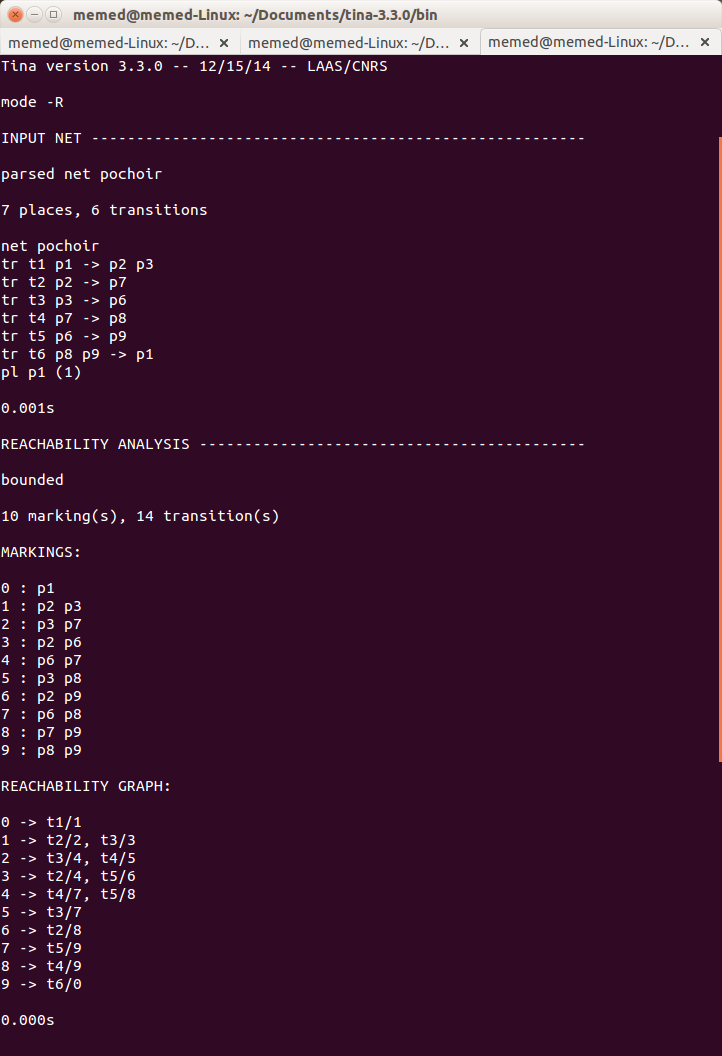
\includegraphics[width=0.25\textwidth]{images/marquage_pochoir.png}
\end{center}

\subsection{Question 6}

\vspace{1cm}

\begin{center}

{\Huge C}\qquad =\qquad $\bordermatrix{
&t_1&t_2&t_3&t_4&t_5&t_6\cr
P_1&-1&0&0&0&0&1\cr
P_2&1&-1&0&0&0&0\cr
P_3&1&0&-1&0&0&0\cr
P_4&0&1&0&-1&0&0\cr
P_5&0&0&1&0&-1&0\cr
P_6&0&0&0&1&0&-1\cr
P_7&0&0&0&0&1&-1\cr
}$

\end{center}

\subsection{Question 7}
On va utiliser l'algorithme de Farkas pour calculer les P-semi flots.

\begin{center}

$\bordermatrix{
&t_1&t_2&t_3&t_4&t_5&t_6\cr
P_1&-1&0&0&0&0&1\cr
P_2&1&-1&0&0&0&0\cr
P_3&1&0&-1&0&0&0\cr
P_4&0&1&0&-1&0&0\cr
P_5&0&0&1&0&-1&0\cr
P_6&0&0&0&1&0&-1\cr
P_7&0&0&0&0&1&-1\cr
}$

{\Huge $\downarrow$}

$\bordermatrix{
&t_1&t_2&t_3&t_4&t_5&t_6\cr
P_1+P_2&0&-1&0&0&0&1\cr
P_1+P_3&0&0&-1&0&0&1\cr
P_4&0&1&0&-1&0&0\cr
P_5&0&0&1&0&-1&0\cr
P_6&0&0&0&1&0&-1\cr
P_7&0&0&0&0&1&-1\cr
}$

{\Huge $\downarrow$}

$\bordermatrix{
&t_1&t_2&t_3&t_4&t_5&t_6\cr
P_1+P_2+P_4&0&0&0&-1&0&1\cr
P_1+P_3&0&0&-1&0&0&1\cr
P_5&0&0&1&0&-1&0\cr
P_6&0&0&0&1&0&-1\cr
P_7&0&0&0&0&1&-1\cr
}$

{\Huge $\downarrow$}

$\bordermatrix{
&t_1&t_2&t_3&t_4&t_5&t_6\cr
P_1+P_2+P_4+P_6&0&0&0&0&0&0\cr
P_1+P_3+P_5+P_7&0&0&0&0&0&0\cr
}$

\vspace{1cm}

On trouve donc 2 P-semi flots :\\
$f_1 = (1\ 1\ 0\ 1\ 0\ 1\ 0)$\\
$f_2 = (1\ 0\ 1\ 0\ 1\ 0\ 1)$

\end{center}

Ceci est confirmé par le logiciel TINA :
\begin{center}
  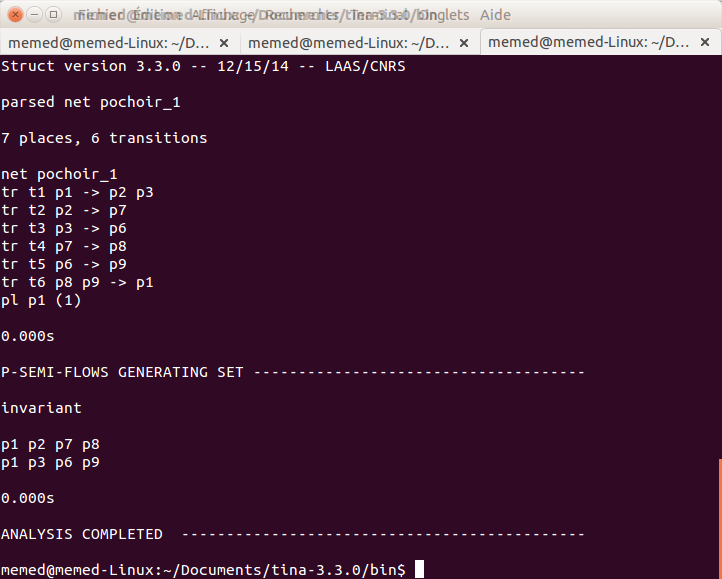
\includegraphics[width=0.25\textwidth]{images/pflot_pochoir.png}
\end{center}

\subsection{Question 8}

Soit $\{M\}$ l'ensemble des marquages accessibles du reseau.\\
Soit $\{t\}$ l'ensemble des transitions du reseau.\\
Le graphe des marquages étant sans feuille, c'est à dire que $\forall M_i \in \{M\}\ \exists t_k \in\{t\} : M_i[t_k>M_j\ avec\ M_j\in \{M\}$ \\
Le réseau est donc sans blocage.

\subsection{Question 9}

\begin{itemize}
  \item Chaque place $P_i$ possède une et une seule transition d'entrée et une et une seule transition de sortie, donc le réseau est un graphe d'événement.
  \item $s_1 = P_1 \rightarrow P_2 \rightarrow P_4 \rightarrow P_6 \rightarrow P_1$ est un circuit élémentaire
  \item $s_2 = P_1 \rightarrow P_3 \rightarrow P_5 \rightarrow P_7 \rightarrow P_1$ est un circuit élémentaire
\end{itemize}

\newpage

\section{Exercice 2 - Protocole de communication}
\subsection{Question 1}
 Le protocole peut être décrit par le réseau suivant : \\

\begin{comment}
\begin{figure}[H]
  \centering
  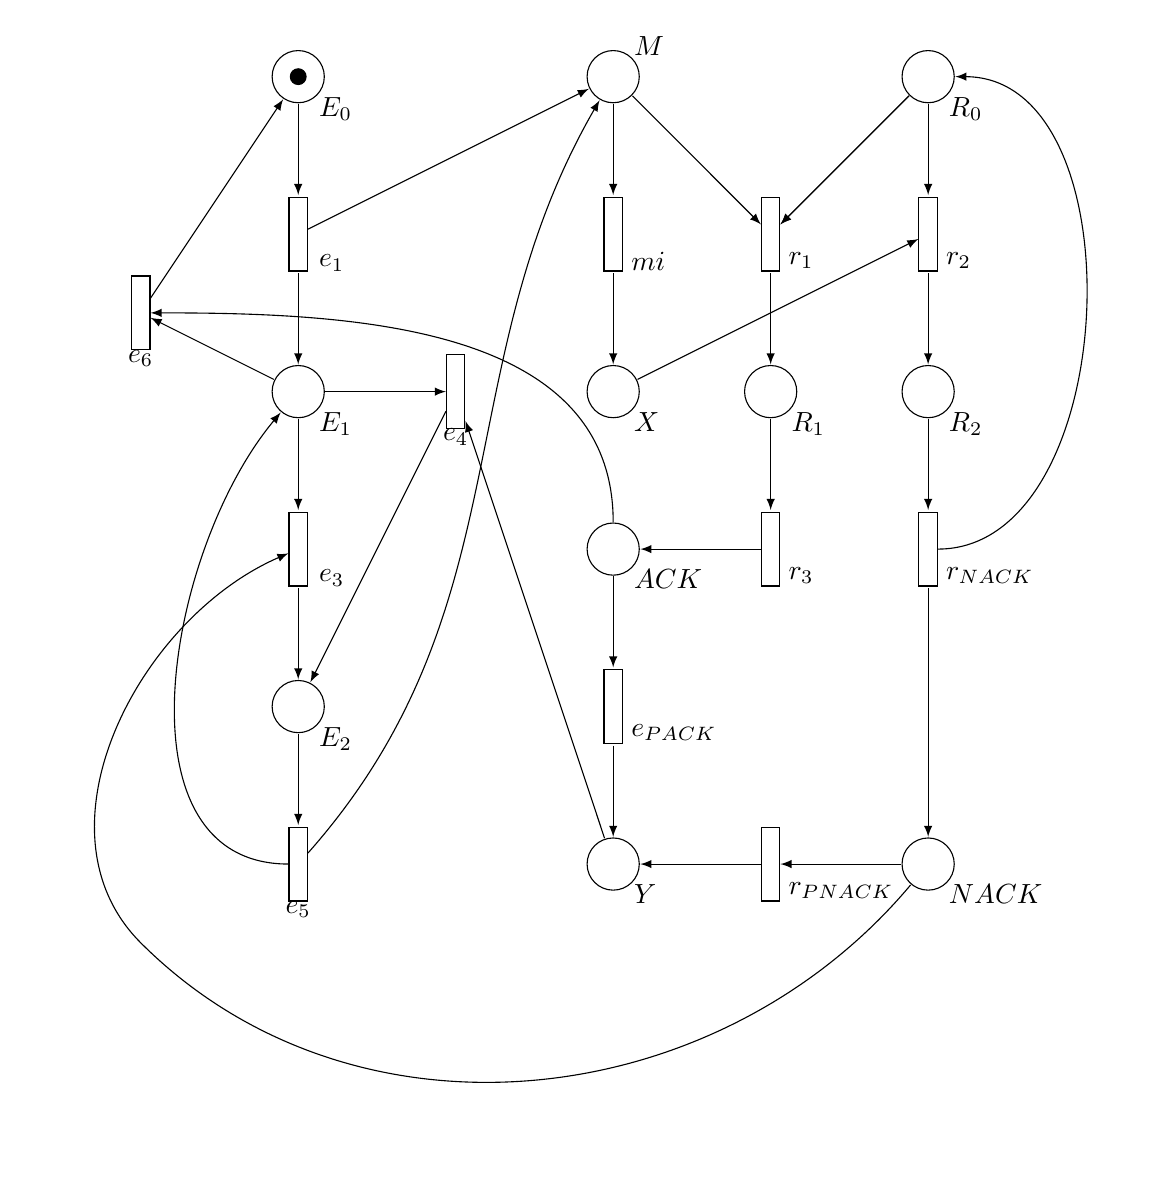
\begin{tikzpicture}
    % Liste des places
    \draw (-4,4) node[below right = 4pt] {$E_0$};
    \node[draw,circle,scale=2] (E0) at (-4, 4) {};
    \draw (-4,0) node[below right = 4pt] {$E_1$};
    \node[draw,circle,scale=2] (E1) at (-4, 0) {};
    \draw (-4,-4) node[below right = 4pt] {$E_2$};
    \node[draw,circle,scale=2] (E2) at (-4, -4) {};
    \draw (0,4) node[above right = 4pt] {$M$};
    \node[draw,circle,scale=2] (M) at (0, 4) {};
    \draw (0,0) node[below right = 4pt] {$X$};
    \node[draw,circle,scale=2] (X) at (0, 0) {};
    \draw (0,-2) node[below right = 4pt] {$ACK$};
    \node[draw,circle,scale=2] (ACK) at (0, -2) {};
    \draw (0,-6) node[below right = 4pt] {$Y$};
    \node[draw,circle,scale=2] (Y) at (0,-6) {};
    \draw (2,0) node[below right = 4pt] {$R_1$};
    \node[draw,circle,scale=2] (R1) at (2, 0) {};
    \draw (4,4) node[below right = 4pt] {$R_0$};
    \node[draw,circle,scale=2] (R0) at (4, 4) {};
    \draw (4,0) node[below right = 4pt] {$R_2$};
    \node[draw,circle,scale=2] (R2) at (4,0) {};
    \draw (4,-6) node[below right = 4pt] {$NACK$};
    \node[draw,circle,scale=2] (NACK) at (4,-6) {};

    % Liste des transitions
    \draw (-6,1) node[below = 10pt] {$e_6$};
    \node[draw,rectangle,yscale=4] (e6) at (-6, 1) {};
    \draw (-4,2) node[below right = 4pt] {$e_1$};
    \node[draw,rectangle,yscale=4] (e1) at (-4, 2) {};
    \draw (-4,-2) node[below right= 4pt] {$e_3$};
    \node[draw,rectangle,yscale=4] (e3) at (-4, -2) {};
    \draw (-4,-6) node[below = 10pt] {$e_5$};
    \node[draw,rectangle,yscale=4] (e5) at (-4, -6) {};
    \draw (-2,0) node[below = 10pt] {$e_4$};
    \node[draw,rectangle,yscale=4] (e4) at (-2, 0) {};
    \draw (0,2) node[below right = 3pt] {$mi$};
    \node[draw,rectangle,yscale=4] (mi) at (0, 2) {};
    \draw (0,-4) node[below right = 3pt] {$e_{PACK}$};
    \node[draw,rectangle,yscale=4] (epa) at (0, -4) {};
    \draw (2,2) node[below right = 3pt] {$r_1$};
    \node[draw,rectangle,yscale=4] (r1) at (2, 2) {};
    \draw (2,-2) node[below right = 3pt] {$r_3$};
    \node[draw,rectangle,yscale=4] (r3) at (2, -2) {};
    \draw (2,-6) node[below right = 3pt] {$r_{PNACK}$};
    \node[draw,rectangle,yscale=4] (rpn) at (2, -6) {};
    \draw (4,2) node[below right = 3pt] {$r_2$};
    \node[draw,rectangle,yscale=4] (r2) at (4, 2) {};
    \draw (4,-2) node[below right = 3pt] {$r_{NACK}$};
    \node[draw,rectangle,yscale=4] (rn) at (4, -2) {};


    % Liste des arcs
    \draw[->,>=latex] (E0) -- (e1);
    \draw[->,>=latex] (e1) -- (E1);
    \draw[->,>=latex] (e1) -- (M);
    \draw[->,>=latex] (E1) -- (e6);
    \draw[->,>=latex] (E1) -- (e4);
    \draw[->,>=latex] (E1) -- (e3);
    \draw[->,>=latex] (M) -- (mi);
    \draw[->,>=latex] (M) -- (r1);
    \draw[->,>=latex] (e6) -- (E0);
    \draw[->,>=latex] (e4) -- (E2);
    \draw[->,>=latex] (e3) -- (E2);
    \draw[->,>=latex] (mi) -- (X);
    \draw[->,>=latex] (r1) -- (R1);
    \draw[->,>=latex] (E2) -- (e5);
    \draw[->,>=latex] (X) -- (r2);
    \draw[->,>=latex] (R1) -- (r3);
    \draw[->,>=latex] (e5) to[out=180,in=230] (E1);
    \draw[->,>=latex] (e5) to[in=240] (M);
    \draw[->,>=latex] (r2) -- (R2);
    \draw[->,>=latex] (r3) -- (ACK);
    \draw[->,>=latex] (R2) -- (rn);
    \draw[->,>=latex] (ACK) -- (epa);
    \draw[->,>=latex] (ACK) to[out=90,in=0] (e6);
    \draw[->,>=latex] (rn) -- (NACK);
    \draw[->,>=latex] (rn) to[out=0,in=0] (R0);
    \draw[->,>=latex] (epa) -- (Y);
    \draw[->,>=latex] (NACK) -- (rpn);
    \draw[->,>=latex] (NACK) to[out=230,in=-45] (-6,-7) to[out=135,in=200] (e3);
    \draw[->,>=latex] (R0) -- (r1);
    \draw[->,>=latex] (R0) -- (r2);
    \draw[->,>=latex] (Y) -- (e4);
    \draw[->,>=latex] (rpn) -- (Y);
    \draw[->,>=latex] (R0) -- (r1);







    % Marquage 
    \draw [fill](-4,4) circle (0.1) ;
  \end{tikzpicture}
  \caption{Réseau de petri associé au protocole de communication} \label{fig:M1}
\end{figure}

\end{comment}

\begin{figure}[H]
  \centering
  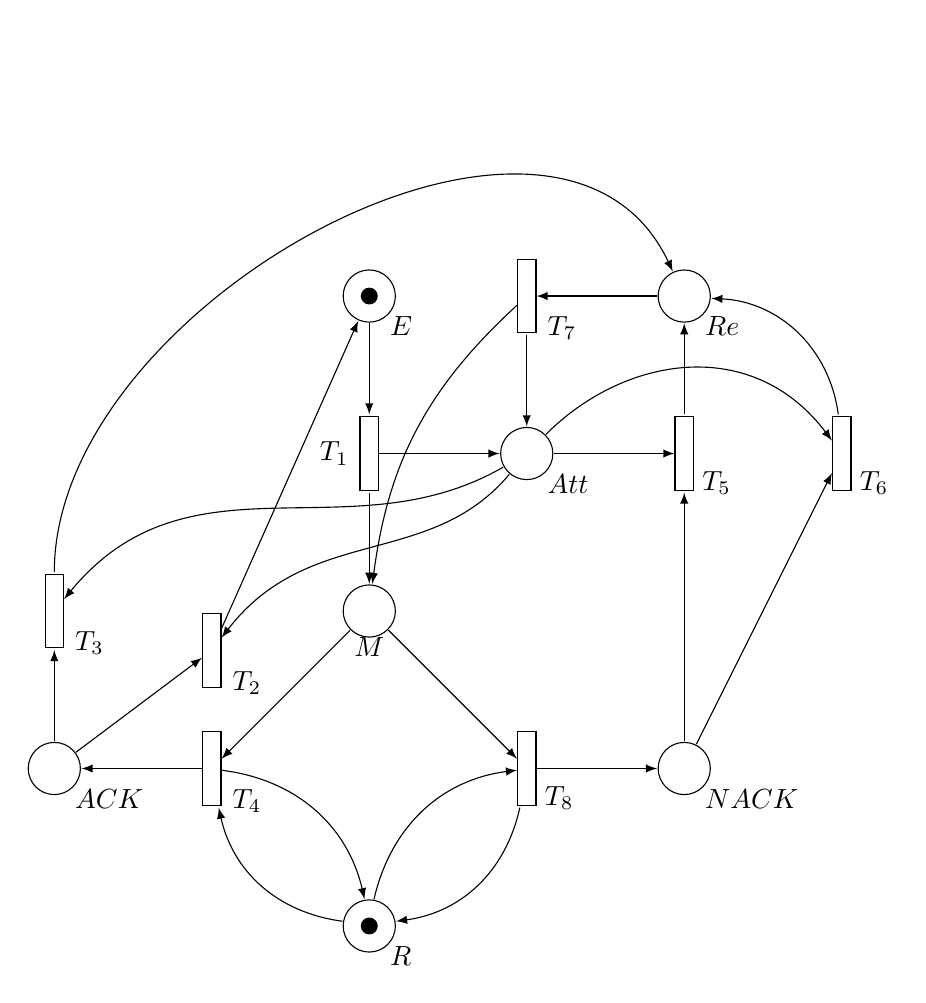
\begin{tikzpicture}
    % Liste des places
    \draw (-2,4) node[below right = 4pt] {$E$};
    \node[draw,circle,scale=2] (E) at (-2, 4) {};
    \draw (-6,-2) node[below right = 4pt] {$ACK$};
    \node[draw,circle,scale=2] (ACK) at (-6, -2) {};
    \draw (-2,0) node[below = 6pt] {$M$};
    \node[draw,circle,scale=2] (M) at (-2,0) {};
    \draw (-2,-4) node[below right = 4pt] {$R$};
    \node[draw,circle,scale=2] (R) at (-2, -4) {};
    \draw (0,2) node[below right = 4pt] {$Att$};
    \node[draw,circle,scale=2] (At) at (0, 2) {};
    \draw (2,4) node[below right = 4pt] {$Re$};
    \node[draw,circle,scale=2] (Re) at (2,4) {};
    \draw (2,-2) node[below right = 4pt] {$NACK$};
    \node[draw,circle,scale=2] (NACK) at (2,-2) {};

    % Liste des transitions
    \draw (-6,0) node[below right= 4pt] {$T_3$};
    \node[draw,rectangle,yscale=4] (T3) at (-6, 0) {};
    \draw (-4,-0.5) node[below right = 4pt] {$T_2$};
    \node[draw,rectangle,yscale=4] (T2) at (-4, -0.5) {};
    \draw (-4,-2) node[below right= 4pt] {$T_4$};
    \node[draw,rectangle,yscale=4] (T4) at (-4, -2) {};
    \draw (-2,2) node[left = 4pt] {$T_1$};
    \node[draw,rectangle,yscale=4] (T1) at (-2, 2) {};
    \draw (0,4) node[below right= 4pt] {$T_7$};
    \node[draw,rectangle,yscale=4] (T7) at (0, 4) {};
    \draw (0,-2) node[below right = 3pt] {$T_8$};
    \node[draw,rectangle,yscale=4] (T8) at (0, -2) {};
    \draw (2,2) node[below right = 3pt] {$T_5$};
    \node[draw,rectangle,yscale=4] (T5) at (2, 2) {};
    \draw (4,2) node[below right = 3pt] {$T_6$};
    \node[draw,rectangle,yscale=4] (T6) at (4, 2) {};


    % Liste des arcs
    \draw[->,>=latex] (E) -- (T1);
    \draw[->,>=latex] (T1) -- (M);
    \draw[->,>=latex] (T1) -- (At);
    \draw[->,>=latex] (M) -- (T4);
    \draw[->,>=latex] (M) -- (T8);
    \draw[->,>=latex] (At) to[out=210,in=45] (T3);
    \draw[->,>=latex] (At) to[out=230,in=45] (T2);
    \draw[->,>=latex] (At) -- (T5);
    \draw[->,>=latex] (At) to[out=45, in=135] (T6);
    \draw[->,>=latex] (T4) -- (ACK);
    \draw[->,>=latex] (T4) to[bend left=35] (R);
    \draw[->,>=latex] (T8) -- (NACK);
    \draw[->,>=latex] (T8) to[bend left=35] (R);
    \draw[->,>=latex] (T3) to[out=90,in=115](Re);
    \draw[->,>=latex] (T2) -- (E);
    \draw[->,>=latex] (T5) -- (Re);
    \draw[->,>=latex] (T6) to[bend right=40] (Re);
    \draw[->,>=latex] (ACK) -- (T3);
    \draw[->,>=latex] (ACK) -- (T2);
    \draw[->,>=latex] (R) to[bend left=35] (T4);
    \draw[->,>=latex] (R) to[bend left=35] (T8);
    \draw[->,>=latex] (NACK) -- (T5);
    \draw[->,>=latex] (NACK) -- (T6);
    \draw[->,>=latex] (Re) -- (T7);
    \draw[->,>=latex] (T7) -- (At);
    \draw[->,>=latex] (T7) to[bend right=20] (M);

    %Marquage
    \draw [fill](-2,4) circle (0.1) ;
    \draw [fill](-2,-4) circle (0.1) ;

  \end{tikzpicture}
  \caption{Réseau de petri associé au protocole de communication} \label{fig:M1}
\end{figure}

\newpage

\subsection{Question 2}

Nous allons représenter le marquagepar un vecteur de la forme :\\
\begin{center}
  (E Att M Re ACK NACK R)\\
\end{center}
où chaque symbole i correspond au nombre de jeton contenu dans la place i.\\
Ainsi $M_0 = (1\ 0\ 0\ 0\ 0\ 0\ 1)$ indique qu'il y a un jeton en E et en R.

\begin{figure}[H]
  \centering
  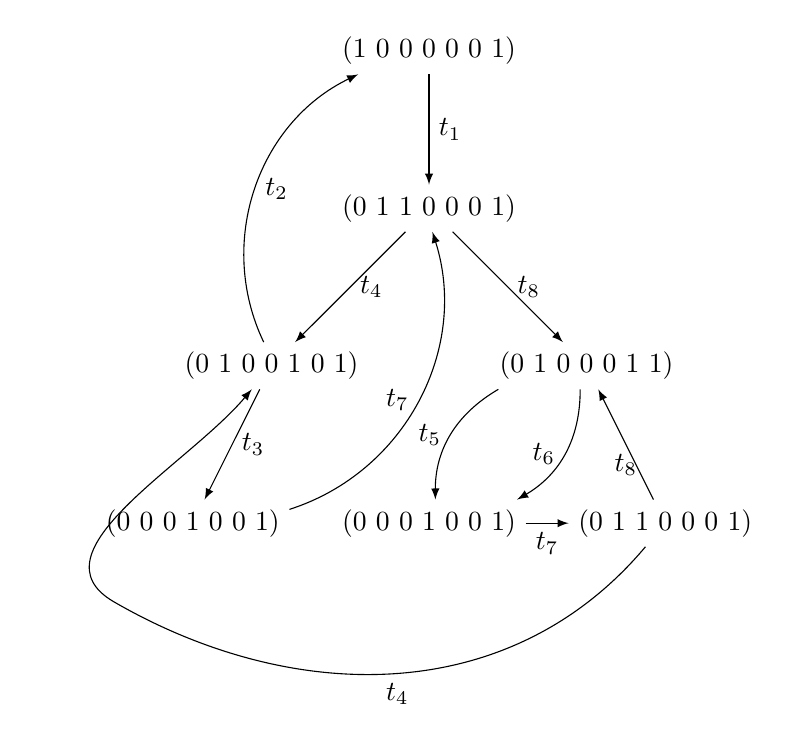
\begin{tikzpicture}
    % Liste des Marquage
    \node (M0) at (0,6) {$(1\ 0\ 0\ 0\ 0\ 0\ 1)$};
    \node (M1) at (0,4) {$(0\ 1\ 1\ 0\ 0\ 0\ 1)$};
    \node (M2) at (-2,2) {$(0\ 1\ 0\ 0\ 1\ 0\ 1)$};
    \node (M3) at (2,2) {$(0\ 1\ 0\ 0\ 0\ 1\ 1)$};
    \node (M4) at (-3,0) {$(0\ 0\ 0\ 1\ 0\ 0\ 1)$};
    \node (M5) at (0,0) {$(0\ 0\ 0\ 1\ 0\ 0\ 1)$};
    \node (M6) at (3,0) {$(0\ 1\ 1\ 0\ 0\ 0\ 1)$};
  

    % Liste des arcs
    \draw[->,>=latex] (M0) -- (M1) node[midway, right]{$t_1$};
    \draw[->,>=latex] (M1) -- (M2) node[midway, right]{$t_4$};
    \draw[->,>=latex] (M1) -- (M3) node[midway, right]{$t_8$};
    \draw[->,>=latex] (M2) to[bend left=45] node[midway, right]{$t_2$} (M0);
    \draw[->,>=latex] (M2) -- (M4) node[midway, right]{$t_3$};
    \draw[->,>=latex] (M3) to[bend right=30] node[midway, left]{$t_5$} (M5);
    \draw[->,>=latex] (M3) to[bend left=30]  node[midway, left]{$t_6$} (M5);
    \draw[->,>=latex] (M4) to[bend right=45] node[midway,left]{$t_7$} (M1);
    \draw[->,>=latex] (M5) -- (M6) node[midway, below]{$t_7$};
    \draw[->,>=latex] (M6) to[out=230,in=-30] node[midway, below]{$t_4$} (-4,-1) to[out=150,in=230] (M2);
    \draw[->,>=latex] (M6) -- (M3) node[midway, below]{$t_8$};

  \end{tikzpicture}
  \caption{Graphe des marquages accessibles} \label{fig:M10}
\end{figure}

\subsection{Question 3}

On a dans notre réseau :
\begin{center}
  $a\ =\ T_1\ et\ b\ =\ T_4$
\end{center}

Lors de l'émission d'un message m par l'émetteur, $T_1$ fait transité |m| caractères.\\
On va considérer que l'ensemble du message est reconnu et accepté par le recepteur.\\
Ainsi, $T_4$ fait également transité |m| caractère.\\
Le recepteur envoie alors un ACK et retourne au repos.\\
A ce moment, l'envoie du ACK peut être perturber et transformer en Y. L'emetteur recevant un Y se mat alors en état de réémission et renvoie le message m.\\
Le recepteur le reçoit donc de nouveau.\\
En considerant que le message est reconnu par le recepteur $T_4$ fait à nouveau transité |m| caractère.\\
Le récepteur envoie à nouveau un ACK et nous allons considerer qu'il n'est pas perturber et donc reçu par l'émetteur.\\
Les deux retourne donc à l'état de repos.\\

En notant $w$ la ligne décrite ci-dessus, on a $|T_1|_w = |m|$ et $|T_4|_w = 2|m|$\\
On a donc bien :
\begin{center}
  $|a|_w < |b|_w$
\end{center}

\subsection{Question 4}


\subsection{Question 5}

\vspace{1cm}

\begin{center}

{\Huge C}\qquad =\qquad $\bordermatrix{
    &t_1 &t_2 &t_3 &t_4 &t_5 &t_6 &t_7 &t_8\cr
E   & -1& 1 & 0 & 0 & 0 & 0 & 0 & 0\cr
Att & 1 &-1 &-1 & 0 &-1 &-1 & 1 & 0\cr
M   & 1 & 0 & 0 &-1 & 0 & 0 & 1 &-1\cr
NACK& 0 & 0 & 0 & 0 &-1 &-1 & 0 & 1\cr
ACK & 0 &-1 &-1 & 1 & 0 & 0 & 0 & 0\cr
R   & 0 & 0 & 0 & 0 & 0 & 0 & 0 & 0\cr
Re  & 0 & 0 & 1 & 0 & 1 & 1 &-1 & 0\cr
}$

\end{center}

\subsection{Question 6}
Soit $F=(f_1\ f_2\ f_3\ f_4\ f_5\ f_6\ f_7)$ le vecteur générique de T-flots.\\
On cherche : 
\begin{center}

$\begin{pmatrix}
-1 & 1 & 0 & 0 & 0 & 0 & 0 & 0\\
 1 &-1 &-1 & 0 &-1 &-1 & 1 & 0\\
 1 & 0 & 0 &-1 & 0 & 0 & 1 &-1\\
 0 & 0 & 0 & 0 &-1 & 0 & 1 & 1\\
 0 &-1 &-1 & 1 & 0 &-1 & 0 & 0\\
 0 & 0 & 0 & 0 & 0 & 0 & 0 & 0\\
 0 & 0 & 1 & 0 & 1 & 1 &-1 & 0
\end{pmatrix}
\begin{pmatrix}
f_1\\
f_2\\ 
f_3\\ 
f_4\\ 
f_5\\ 
f_6\\ 
f_7
\end{pmatrix}
=0
$

\vspace{0.5cm}

$\rightarrow 
\begin{cases}
f_1 = f_2\\
f_1 - f_2 - f_3 - f_5 - f_6 + f_7 = 0\\
f_1 - f_4 + f_7 - f_8 = 0\\
-f_5 - f_6 + f_8 = 0\\
-f_2 - f_3 + f_4 = 0\\
f_3 + f_5 + f_6 - f_7 = 0
\end{cases}$

\vspace{0.5cm}

$\rightarrow 
\begin{cases}
f_1 = f_2\\
- f_3 - f_5 - f_6 + f_7 = 0\\
f_1 - f_4 + f_7 - f_8 = 0\\
-f_5 - f_6 + f_8 = 0\\
-f_2 - f_3 + f_4 = 0\\
f_3 + f_5 + f_6 - f_7 = 0
\end{cases}$

\vspace{0.5cm}

$\rightarrow 
\begin{cases}
f_2 = f_1\\
f_8 = f_5 + f_6\\
f_7 = f_3 + f_5 + f_6\\
f_4 = f_1 + f_3
\end{cases}$

\newpage

Ainsi, le vecteur générique de T-flots $F=(f_1\ \ f_1\ \ f_3\ \ f_1+f_3\ \ f_5\ \ f_6\ \ f_3+f_5+f_6\ \ f_5+f_6)$\\
On obtient donc 4 T-flots :\\
$F_1\ =\ (1\ 1\ 0\ 1\ 0\ 0\ 0\ 0)$\\
$F_2\ =\ (0\ 0\ 1\ 1\ 0\ 0\ 1\ 0)$\\
$F_3\ =\ (0\ 0\ 0\ 0\ 1\ 0\ 1\ 1)$\\
$F_4\ =\ (0\ 0\ 0\ 0\ 0\ 1\ 1\ 1)$\\

\vspace{0.5cm}

Ce qui est confirmé par le logiciel TINA :\\
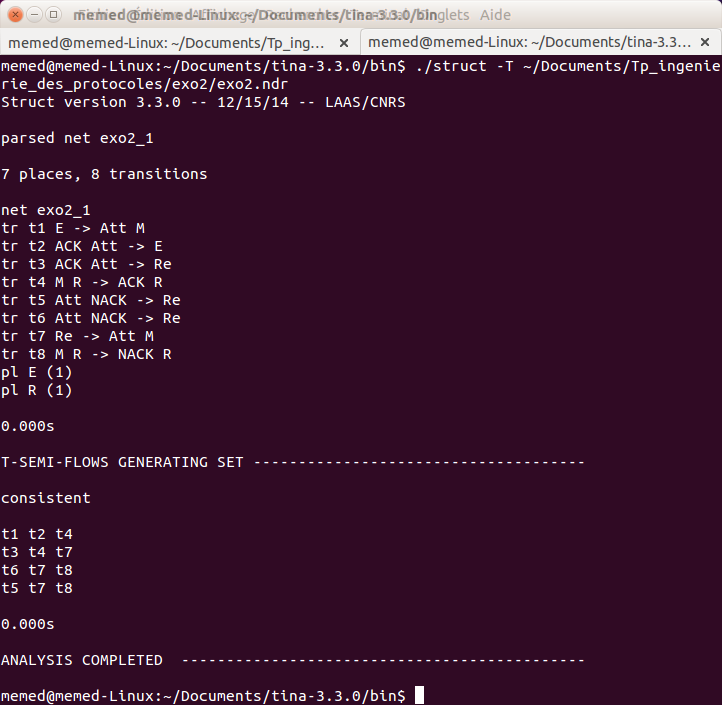
\includegraphics[width=0.35\textwidth]{images/tflots2.png}\\
\end{center}

Les séquences répétitives du réseau :\\
Les T-flots nous donnent les composantes répétitives $T(S_i)$, c'est à dire l’ensemble des
transitions qui apparaissent dans la séquence répétitive $S_i$.\\
Il nous faut donc remettre les transitions de chaque composante dans le bon ordre pour obtenir les séquence répétitive.\\
$F_1\ =\ (1\ 1\ 0\ 1\ 0\ 0\ 0\ 0)\ \rightarrow\ T(S_1) = {t_1,\ t_2,\ t_4} \rightarrow S_1 =t_1,\ t_4,\ t_2$\\
$F_2\ =\ (0\ 0\ 1\ 1\ 0\ 0\ 1\ 0)\ \rightarrow\ T(S_2) = {t_3,\ t_4,\ t_7} \rightarrow S_1 =t_3,\ t_7,\ t_4$\\
$F_3\ =\ (0\ 0\ 0\ 0\ 1\ 0\ 1\ 1)\ \rightarrow\ T(S_1) = {t_5,\ t_7,\ t_8} \rightarrow S_1 =t_5,\ t_7,\ t_8$\\
$F_4\ =\ (0\ 0\ 0\ 0\ 0\ 1\ 1\ 1)\ \rightarrow\ T(S_1) = {t_6,\ t_7,\ t_8} \rightarrow S_1 =t_6,\ t_7,\ t_8$\\

\subsection{Question 7}

Soit $P=(p_E\ p_{Att}\ p_M\ p_{NACK}\ p_{ACK}\ p_R\ p_{Re})$ le vecteur générique de P-semi-flots.\\
Les P-semi-flots du reseau sont :
\begin{itemize}
\item $P_1$ = (0 0 0 0 0 1 0)
\item $P_2$ = (1 1 0 0 0 0 1)
\item $P_3$ = (1 0 1 1 1 0 1)
\end{itemize}

Chaque P-semi-flot $P_i$ nous donne une composante conservatrice du réseau, et par définition, toute place $p$ de cette composante est borné et l’on a : $M(p) \leq (^TP_i \cdot M_0)/p_j$.\\
Ainsi, on a :
\begin{itemize}
\item $P_1 \rightarrow R$ est bornée et $M(R) \leq (^TP_1 \cdot M_0)/p_{1_R} = 1$

\item $P_2 \rightarrow 
\begin{cases}
$E est bornée et  $M(E) \leq (^TP_2 \cdot M_0)/p_{2_R} = 1\\
$Att est bornée et  $M(Att) \leq (^TP_2 \cdot M_0)/p_{2_{Att}} = 1\\
$E est bornée et  $M(Re) \leq (^TP_2 \cdot M_0)/p_{2_{Re}} = 1
\end{cases}$

\item $P_3 \rightarrow 
\begin{cases}
$M est bornée et  $M(M) \leq (^TP_3 \cdot M_0)/p_{3_M} = 1\\
$NACK est bornée et  $M(NACK) \leq (^TP_3 \cdot M_0)/p_{3_{NACK}} = 1\\
$ACK est bornée et  $M(ACK) \leq (^TP_3 \cdot M_0)/p_{3_{ACK}} = 1
\end{cases}$

\end{itemize}

Donc toute les places du réseau sont bornée, ce qui implique que le réseau est borné.

\subsection{Question 8}
Nous avons choisit d'étiqueter les transitions du réseau de la manière suivante :
\begin{itemize}
\item $T_1$ reçoit l'étiquette $M_E$ pour ``Message envoyé''
\item $T_2$ reçoit l'étiquette $M_A$ pour ``Message ACK envoyé''
\item $T_3$ reçoit l'étiquette $Y_A$ pour ``Message ACK pertubé en Y''
\item $T_4$ reçoit l'étiquette $M_R$ pour ``Message reconnu''
\item $T_5$ reçoit l'étiquette $Y_N$ pour ``Message NACK pertubé en Y''
\item $T_6$ reçoit l'étiquette $M_N$ pour ``Message NACK envoyé''
\item $T_7$ reçoit l'étiquette $M_{Re}$ pour ``Message renvoyé''
\item $T_8$ reçoit l'étiquette $M_P$ pour ``Message Perturbé''
\end{itemize}

\begin{comment}

\begin{figure}[H]
  \centering
  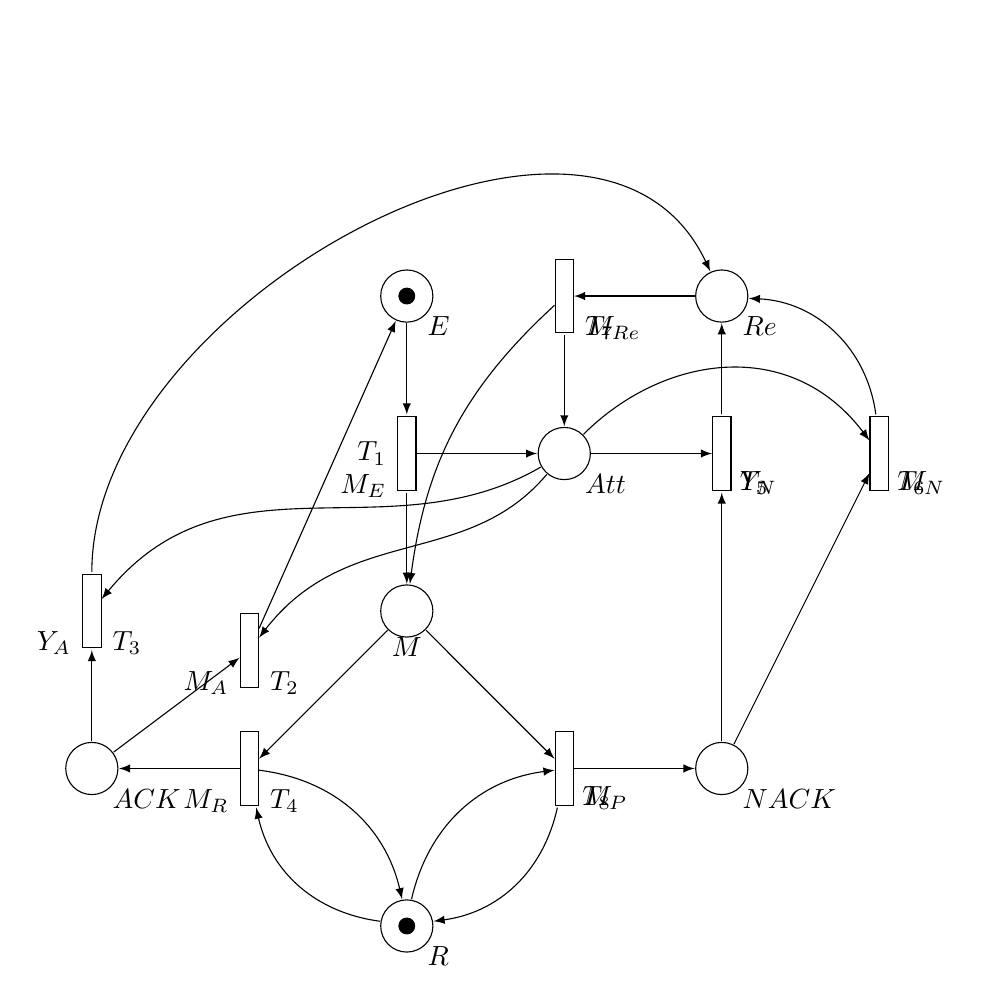
\begin{tikzpicture}
    % Liste des places
    \draw (-2,4) node[below right = 4pt] {$E$};
    \node[draw,circle,scale=2] (E) at (-2, 4) {};
    \draw (-6,-2) node[below right = 4pt] {$ACK$};
    \node[draw,circle,scale=2] (ACK) at (-6, -2) {};
    \draw (-2,0) node[below = 6pt] {$M$};
    \node[draw,circle,scale=2] (M) at (-2,0) {};
    \draw (-2,-4) node[below right = 4pt] {$R$};
    \node[draw,circle,scale=2] (R) at (-2, -4) {};
    \draw (0,2) node[below right = 4pt] {$Att$};
    \node[draw,circle,scale=2] (At) at (0, 2) {};
    \draw (2,4) node[below right = 4pt] {$Re$};
    \node[draw,circle,scale=2] (Re) at (2,4) {};
    \draw (2,-2) node[below right = 4pt] {$NACK$};
    \node[draw,circle,scale=2] (NACK) at (2,-2) {};

    % Liste des transitions
    \draw (-6,0) node[below right= 4pt] {$T_3$};
    \draw (-6,0) node[below left= 4pt] {$Y_A$};
    \node[draw,rectangle,yscale=4] (T3) at (-6, 0) {};
    \draw (-4,-0.5) node[below right = 4pt] {$T_2$};
    \draw (-4,-0.5) node[below left = 4pt] {$M_A$};
    \node[draw,rectangle,yscale=4] (T2) at (-4, -0.5) {};
    \draw (-4,-2) node[below right= 4pt] {$T_4$};
    \draw (-4,-2) node[below left= 4pt] {$M_R$};
    \node[draw,rectangle,yscale=4] (T4) at (-4, -2) {};
    \draw (-2,2) node[left = 4pt] {$T_1$};
    \draw (-2,2) node[below left = 4pt] {$M_E$};
    \node[draw,rectangle,yscale=4] (T1) at (-2, 2) {};
    \draw (0,4) node[below right= 4pt] {$T_7$};
    \draw (0,4) node[below right= 4pt] {$M_{Re}$};
    \node[draw,rectangle,yscale=4] (T7) at (0, 4) {};
    \draw (0,-2) node[below right = 3pt] {$T_8$};
    \draw (0,-2) node[below right = 3pt] {$M_P$};
    \node[draw,rectangle,yscale=4] (T8) at (0, -2) {};
    \draw (2,2) node[below right = 3pt] {$T_5$};
    \draw (2,2) node[below right = 3pt] {$Y_N$};
    \node[draw,rectangle,yscale=4] (T5) at (2, 2) {};
    \draw (4,2) node[below right = 3pt] {$T_6$};
    \draw (4,2) node[below right = 3pt] {$M_N$};
    \node[draw,rectangle,yscale=4] (T6) at (4, 2) {};


    % Liste des arcs
    \draw[->,>=latex] (E) -- (T1);
    \draw[->,>=latex] (T1) -- (M);
    \draw[->,>=latex] (T1) -- (At);
    \draw[->,>=latex] (M) -- (T4);
    \draw[->,>=latex] (M) -- (T8);
    \draw[->,>=latex] (At) to[out=210,in=45] (T3);
    \draw[->,>=latex] (At) to[out=230,in=45] (T2);
    \draw[->,>=latex] (At) -- (T5);
    \draw[->,>=latex] (At) to[out=45, in=135] (T6);
    \draw[->,>=latex] (T4) -- (ACK);
    \draw[->,>=latex] (T4) to[bend left=35] (R);
    \draw[->,>=latex] (T8) -- (NACK);
    \draw[->,>=latex] (T8) to[bend left=35] (R);
    \draw[->,>=latex] (T3) to[out=90,in=115](Re);
    \draw[->,>=latex] (T2) -- (E);
    \draw[->,>=latex] (T5) -- (Re);
    \draw[->,>=latex] (T6) to[bend right=40] (Re);
    \draw[->,>=latex] (ACK) -- (T3);
    \draw[->,>=latex] (ACK) -- (T2);
    \draw[->,>=latex] (R) to[bend left=35] (T4);
    \draw[->,>=latex] (R) to[bend left=35] (T8);
    \draw[->,>=latex] (NACK) -- (T5);
    \draw[->,>=latex] (NACK) -- (T6);
    \draw[->,>=latex] (Re) -- (T7);
    \draw[->,>=latex] (T7) -- (At);
    \draw[->,>=latex] (T7) to[bend right=20] (M);

    %Marquage
    \draw [fill](-2,4) circle (0.1) ;
    \draw [fill](-2,-4) circle (0.1) ;

  \end{tikzpicture}
  \caption{Réseau de petri associé au protocole de communication après étiquetage des transitions} \label{fig:M1}
\end{figure}
\end{comment}

On crée le graphe de séquence suivant : \\

\begin{figure}[H]
  \centering
  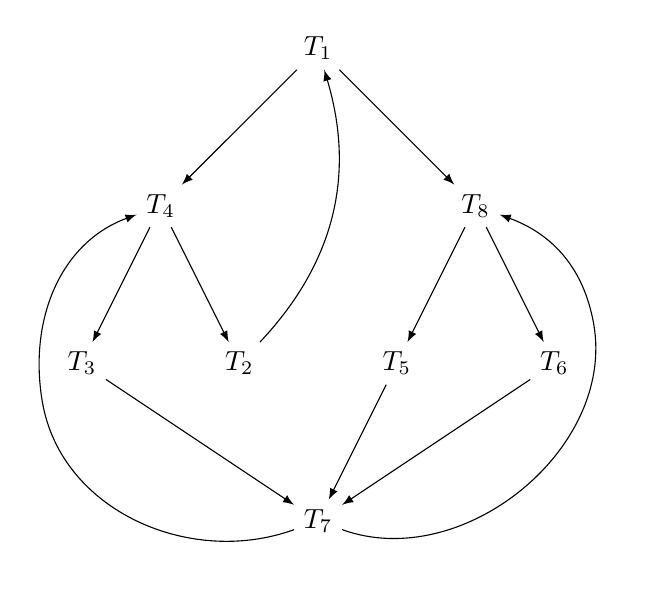
\begin{tikzpicture}
    % Liste des Marquage
    \node (T1) at (0,4) {$T_1$};
    \node (T2) at (-1,0) {$T_2$};
    \node (T3) at (-3,0) {$T_3$};
    \node (T4) at (-2,2) {$T_4$};
    \node (T5) at (1,0) {$T_5$};
    \node (T6) at (3,0) {$T_6$};
    \node (T7) at (0,-2) {$T_7$};
    \node (T8) at (2,2) {$T_8$};
    % Liste des arcs
    \draw[->,>=latex] (T1) -- (T4);
    \draw[->,>=latex] (T1) -- (T8);
    \draw[->,>=latex] (T4) -- (T3);
    \draw[->,>=latex] (T4) -- (T2);
    \draw[->,>=latex] (T8) -- (T5);
    \draw[->,>=latex] (T8) -- (T6);
    \draw[->,>=latex] (T3) -- (T7);
    \draw[->,>=latex] (T2) to[bend right=30] (T1);
    \draw[->,>=latex] (T5) -- (T7);
    \draw[->,>=latex] (T6) -- (T7);
    \draw[->,>=latex] (T7) to[out=200,in=-80] (-3.5,-0.5) to[out=100, in=200] (T4);
    \draw[->,>=latex] (T7) to[out=-20,in=-80] (3.5,0.5) to[out=100, in=-20] (T8);

  \end{tikzpicture}
  \caption{Graphe de séquences} \label{fig:M10}
\end{figure}

Et on déduit le langage définit par l'expression :\\
\begin{center}
$(M_EM_RM_A)^*|M_E[(M_RY_A|M_P(Y_NM_P))M_{Re}]^*$
\end{center}

\subsection{Question 9}

Soit $\{M\}$ l'ensemble des marquage accessible depuis $M_0$\\
Soit $v : \{M\} \rightarrow \mathbb{N}$ l'application telle que :\\
$\forall M_i \in \{M\} : v(M_i) = 1-M_i(E)$\\
Il est clair que $v(M_i) = 0 \Leftrightarrow M_i = M_0$\\
\vspace{0.5cm}
donc $v$ est une norme pour $M_0$ \\
Alors $M_0$ est un etat d'accueil et le reseau est réinitialisable.


\subsection{Question 10}
$\forall M_i, \exists t$ une transition franchissable depuis $M_i$.\\
D'où le réseau est sans blocage.

\subsection{Question 11}

On peut trouver une séquence $S$ qui contienne tout les transitions.\\
ex : $S = t_1,t_4,t_3,t_7,t_8,t_5,t_7,t_8,t_6,t_4,t_2$\\
Donc le réseau est vivant

\subsection{Question 12}
Le graphe des marquage ne contient pas de noeud feuille donc le réseau est bien sans blocage.\\
Il existe un chemin dans le graphe passant par toutes les transitions donc le réseau est bien vivant.\\
$\forall M_i, \exists c$ un chemin de $M_i$ à $M_0$ donc le reseau est réinitialisable.

\subsection{Question 13}


\section{Exercice 3 - Un protocole de connexion-deconnexion}
\subsection{Question 1}

\vspace{1cm}

\begin{center}

{\Huge C}\qquad =\qquad $\bordermatrix{
   &a_0&a_1&a_2&a_3&a_4&a_5&b_1&b_2&b_3&b_4&b_5\cr
A_0&-1 & 0 & 0 & 1 & 1 & 1 & 0 & 0 & 0 & 0 & 0\cr
A_1& 1 &-1 & 0 & 0 & 0 & 0 & 0 & 0 & 0 & 0 & 0\cr
A_2& 0 & 1 &-1 &-1 & 0 & 0 & 0 & 0 & 0 & 0 & 0\cr
A_3& 0 & 0 & 1 & 0 &-1 &-1 & 0 & 0 & 0 & 0 & 0\cr
B_1& 0 & 0 & 0 & 0 & 0 & 0 &-1 & 0 & 1 & 1 & 1\cr
B_2& 0 & 0 & 0 & 0 & 0 & 0 & 1 &-1 &-1 & 0 & 0\cr
B_3& 0 & 0 & 0 & 0 & 0 & 0 & 0 & 1 & 0 &-1 &-1\cr
CC & 0 &-1 & 0 & 0 & 0 & 0 & 1 & 0 & 0 & 0 & 0\cr
CDA& 0 & 0 & 0 & 0 &-1 & 0 & 0 & 0 & 1 & 0 & 0\cr
CDB& 0 & 0 & 0 & 1 & 0 & 0 & 0 & 0 & 0 &-1 & 0\cr
DC & 1 & 0 & 0 & 0 & 0 & 0 &-1 & 0 & 0 & 0 & 0\cr
DDA& 0 & 0 & 1 & 0 & 0 & 0 & 0 & 0 &-1 & 0 &-1\cr
DDB& 0 & 0 & 0 &-1 & 0 &-1 & 0 & 1 & 0 & 0 & 0\cr
}$

\end{center}

\subsection{Question 2}

Soit $F=(f_{A_0}\ f_{A_1}\ f_{A_2}\ f_{A_3}\ f_{B_1}\ f_{B_2}\ f_{B_3}\ f_{CC}\ f_{CDA}\ f_{CDB}\ f_{DC}\ f_{DDA}\ f_{DDB})$ le vecteur générique de P-semi-flots.

TINA nous donne 6 P-semi-flots :\\
$F_1\ =\ (1\ 1\ 1\ 1\ 0\ 0\ 0\ 0\ 0\ 0\ 0\ 0\ 0)$\\
$F_2\ =\ (1\ 0\ 1\ 1\ 0\ 0\ 0\ 1\ 0\ 0\ 1\ 0\ 0)$\\
$F_3\ =\ (0\ 0\ 1\ 0\ 1\ 0\ 0\ 1\ 0\ 1\ 0\ 1\ 0)$\\
$F_4\ =\ (0\ 0\ 0\ 1\ 1\ 1\ 0\ 0\ 0\ 0\ 0\ 0\ 0)$\\
$F_5\ =\ (1\ 0\ 0\ 0\ 0\ 1\ 0\ 0\ 1\ 0\ 1\ 0\ 1)$\\
$F_6\ =\ (1\ 1\ 1\ 0\ 1\ 1\ 0\ 0\ 1\ 1\ 0\ 1\ 1)$\\

\subsection{Question 3}

Soit $F=(f_{a_0}\ f_{a_1}\ f_{a_2}\ f_{a_3}\ f_{a_4}\ f_{a_5}\ f_{b_1}\ f_{b_2}\ f_{b_3}\ f_{b_4}\ f_{b_4})$ le vecteur générique de T-semi-flots.

TINA nous donne 3 T-semi-flots :\\
$F_1\ =\ (1\ 1\ 1\ 0\ 1\ 0\ 1\ 0\ 1\ 0\ 0)$\\
$F_2\ =\ (1\ 1\ 0\ 1\ 0\ 0\ 1\ 1\ 0\ 1\ 0)$\\
$F_3\ =\ (1\ 1\ 1\ 0\ 0\ 1\ 1\ 1\ 0\ 0\ 1)$\\

\newpage

\subsection{Question 4}

Soit $\{M\}$ l'ensemble des marquage accessible depuis $M_0$\\
Soit $v : \{M\} \rightarrow \mathbb{N}$ l'application telle que :\\
$\forall M_i \in \{M\} : v(M_i) = 2-M_i(A_0)-M_i(B_1)$\\
On a $v(M_i) = 0 \Leftrightarrow M_i = M_0$ car toutes les transitions permettant de remettre un jeton en $A_0$ ne peuvent être sensibiliser en même temps que celles qui remettent des jeton dans $B_1$ donc $A_0$ et $B_1$ ne peuvent recevoir un jeton en même temps et le semi-flots nous apprenent que les places sont toutes bornées à 1.\\
donc $\forall M_i,\ si\ M_i(A_0) =1\ et\ M_i(B_1) = 1\ alors\ M_i = M_0$ 
\vspace{0.5cm}
donc $v$ est une norme pour $M_0$ \\
Alors $M_0$ est un etat d'accueil et le reseau est réinitialisable.

\subsection{Question 5}

\begin{itemize}
\item Les P-semi-flots nous apprennent que toutes les places sont bornées à 1.
\item Les T-flots nous apprennent que toutes les transitions sont franchissable depuis un marquage $M_i \in \{M\}$
En outre, le reseau étant réinitiable, on va pouvoir trouver une séquence $S$ qui contienne tout les transitions et qui repasse par $M_0$.\\
ex : $S = a_0,b_1,a_1,a_2,b_3,a_4,a_0,b_1,a_1,b_2,a_3,b_4,a_0,b_1,a_1,a_2,b_2,b_5,a_5$\\
Donc le réseau est vivant
\end{itemize}

\newpage

\section{Exercice 4 - Modelisation d'un programme}
\input{exo4/Exo4}
\section{Exercice 5 - Spécification d'un protocole de communication}
\subsection{Question 1}
 Le protocole peut être décrit par le réseau suivant : \\

\begin{figure}[H]
  \centering
  \begin{tikzpicture}

    % Liste des places
    \draw (-6,2) node[below right = 2pt] {$P_1$};
    \node[draw,circle,scale=2] (P1) at (-6, 2) {};
    \draw (-2,2) node[below right = 2pt] {$P_2$};
    \node[draw,circle,scale=2] (P2) at (-2, 2) {};
    \draw (-4,0) node[below right = 2pt] {$P_3$};
    \node[draw,circle,scale=2] (P3) at (-4,0) {};
    \draw (2,2) node[below right = 2pt] {$P_4$};
    \node[draw,circle,scale=2] (P4) at (2, 2) {};
    \draw (0,0) node[below right = 2pt] {$P_5$};
    \node[draw,circle,scale=2] (P5) at (0,0) {};
    \draw (2,-2) node[below left = 2pt] {$P_6$};
    \node[draw,circle,scale=2] (P6) at (2, -2) {};

    % Liste des transitions
    \draw (-4,2) node[below = 10pt] {$t_1$};
    \node[draw,rectangle,yscale=4] (t1) at (-4, 2) {};
    \draw (2,0) node[below = 10pt] {$t_3$};
    \node[draw,rectangle,yscale=4] (t3) at (2, 0) {};
    \draw (0,2) node[below = 10pt] {$t_2$};
    \node[draw,rectangle,yscale=4] (t2) at (0, 2) {};
    \draw (-6,-0) node[below = 10pt] {$t_5$};
    \node[draw,rectangle,yscale=4] (t5) at (-6, 0) {};
    \draw (4,2) node[below = 10pt] {$t_4$};
    \node[draw,rectangle,yscale=4] (t4) at (4, 2) {};
    
        % Liste des arcs
    \draw[->,>=latex] (P1) -- (t1);
    \draw[->,>=latex] (t1) -- (P3);
    \draw[->,>=latex] (P3) -- (t5);
    \draw[->,>=latex] (t5) -- (P1);
    \draw[->,>=latex] (t1) -- (P2);
    \draw[->,>=latex] (P2) -- (t5);
    \draw[->,>=latex] (P2) -- (t2);
    \draw[->,>=latex] (P5) -- (t2);
    \draw[->,>=latex] (t2) -- (P4);
    \draw[->,>=latex] (P4) -- (t3);
    \draw[->,>=latex] (t3) -- (P6);
    \draw[->,>=latex] (P6) -- (t4);
    \draw[->,>=latex] (P4) -- (t4);
    \draw[->,>=latex] (t4) -- (P5);
    \draw[->,>=latex] (t4) to [out=90,in=90] (P1);

    % Marquage 
    \draw [fill](-6,2) circle (0.1) ;
    \draw [fill](0,0) circle (0.1) ;
  \end{tikzpicture}
  \caption{Réseau de petri associé à l'exercice 5} \label{fig:M5}
\end{figure}

Quand l'utilisateur rentre en communication,l'attente du controleur est symbolisé par le faite qu'il n'y est pas de jeton dans celui-ci.
\section{Exercice 6 - Expression complètement parenthésée}
\subsection{Question 6}
Voici le Rdp permettant de savoir si une expression est bien une expression complètement parenthésée:

Note: L'énoncé étant incorrect, nous avons choisi de modifier la grammaire de la façon suivante afin de mener à bien le reste de l'exercice:

\begin{itemize}
    \item '(' => '(' OU une lettre OU ')'
    \item une lettre => opérateur OU ')'
    \item ')' => ')' OU opérateur OU EOF
    \item opérateur => '(' OU une lettre
\end{itemize}

\begin{figure}[H]
  \centering
  \begin{tikzpicture}
    % Liste des places
    \draw (-6,4) node[below left = 2pt] {$'('$};
    \node[draw,circle,scale=2] (po) at (-6, 4) {};
    \draw (0,2) node[above left = 2pt] {$lettre$};
    \node[draw,circle,scale=2] (lettre) at (0, 2) {};
    \draw (6, 2) node[below right = 2pt] {$operateur$};
    \node[draw,circle,scale=2] (operateur) at (6, 2) {};
    \draw (0,0) node[above right = 2pt] {$')'$};
    \node[draw,circle,scale=2] (pf) at (0, 0) {};
    \draw (6,-4) node[below right = 2pt] {$EOF$};
    \node[draw,circle,scale=2] (EOF) at (6, -4) {};


    % Liste des transitions
    \draw (-6,6) node[below = 10pt] {$t_1$};
    \node[draw,rectangle,yscale=4] (t1) at (-6, 6) {};
    \draw (-3,2) node[below = 10pt] {$t_2$};
    \node[draw,rectangle,yscale=4] (t2) at (-3, 2) {};
    \draw (-3,0) node[below = 10pt] {$t_3$};
    \node[draw,rectangle,yscale=4] (t3) at (-3, 0) {};
    \draw (3,2) node[below = 10pt] {$t_4$};
    \node[draw,rectangle,yscale=4] (t4) at (3, 2) {};
    \draw (3,0) node[below = 10pt] {$t_5$};
    \node[draw,rectangle,yscale=4] (t5) at (3, 0) {};
    \draw (0,-4) node[below = 10pt] {$t_6$};
    \node[draw,rectangle,yscale=4] (t6) at (0, -4) {};
    \draw (3,-2) node[below = 10pt] {$t_7$};
    \node[draw,rectangle,yscale=4] (t7) at (3, -2) {};
    \draw (3,-4) node[below = 10pt] {$t_8$};
    \node[draw,rectangle,yscale=4] (t8) at (3, -4) {};
    \draw (3,4) node[below = 10pt] {$t_9$};
    \node[draw,rectangle,yscale=4] (t9) at (3, 4) {};
    \draw (0,6) node[below = 10pt] {$t_10$};
    \node[draw,rectangle,yscale=4] (t10) at (0, 6) {};



    % Liste des arcs
    \draw[->,>=latex] (po) to[out=135,in=-135] (t1);
    \draw[->,>=latex] (t1) to[out=-45,in=45] (po);
    \draw[->,>=latex] (po) -- (t2);
    \draw[->,>=latex] (t2) -- (lettre);
    \draw[->,>=latex] (po) -- (t3);
    \draw[->,>=latex] (t3) -- (pf);
    \draw[->,>=latex] (lettre) -- (t4);
    \draw[->,>=latex] (t4) -- (operateur);
    \draw[->,>=latex] (lettre) -- (t5);
    \draw[->,>=latex] (t5) -- (pf);
    \draw[->,>=latex] (pf) to[out=-45,in=45] (t6);
    \draw[->,>=latex] (t6) to[out=135,in=-135] (pf);
    \draw[->,>=latex] (pf) -- (t7);
    \draw[->,>=latex] (t7) -- (operateur);
    \draw[->,>=latex] (pf) -- (t8);
    \draw[->,>=latex] (t8) -- (EOF);
    \draw[->,>=latex] (operateur) -- (t9);
    \draw[->,>=latex] (t9) -- (lettre);
    \draw[->,>=latex] (operateur) to[out=90,in=0] (t10);
    \draw[->,>=latex] (t10) -- (po);
    %\draw[->,>=latex] (t6) to[out=-90,in=-90] (P1);

    % Marquage
    \draw [fill](-6,4) circle (0.1) ;
  \end{tikzpicture}
  \caption{Réseau de petri associé à une expression complètement parenthésée} \label{fig:M1}
\end{figure}


\newpage

\section{Exercice 7 - Etude d'un réseau de Petri partuculier}
\subsection{Question 1}
\subsubsection{Question 1.1}

Soit $f=(f_{d_0}\ f_{p_0}\ f_{p_1}\ f_{f_0}\ f_{c_0}\ f_{c'_0})$ le vecteur générique de P-semi-flots.\\
Tina nous donne le p-semi-flot suivant pour le premier schéma :\\
\begin{center}
  $f= (1\ 1\ 1\ 1\ 0\ 0)$

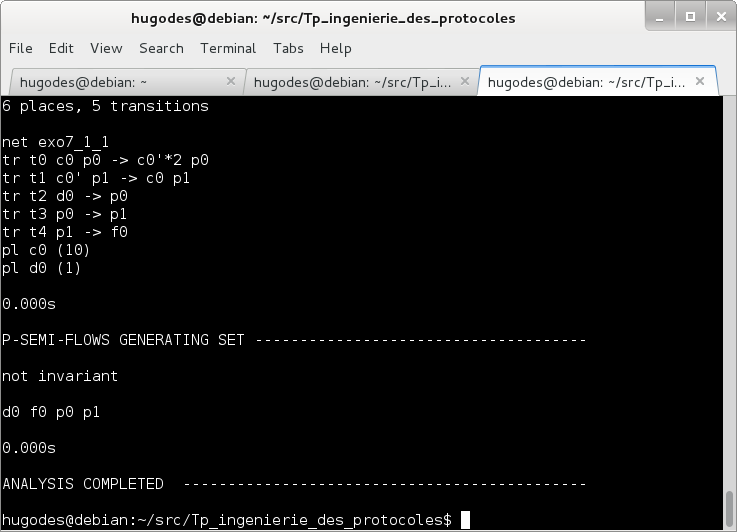
\includegraphics[width=0.7\textwidth]{exo7/tina_7_1.png}\\

\end{center}

On va utiliser l'algorithme de Farkas pour calculer les P-semi flots du premier schéma.

\begin{center}

{\Huge C}\qquad =\qquad $\bordermatrix{
&t_1&t_2&t_3&t_4&t_5\cr
d0&-1&0&0&0&0\cr
p0&1&-1&0&0&0\cr
p1&0&1&-1&0&0\cr
f0&0&0&1&0&0\cr
c0&0&0&0&-1&1\cr
c'0&0&0&0&2&-1\cr
}$

{\Huge $\downarrow$}

$\bordermatrix{
&t_2&t_3&t_4&t_5\cr
d0+p0&-1&0&0&0\cr
p1&1&-1&0&0\cr
f0&0&1&0&0\cr
c0&0&0&-1&1\cr
c'0&0&0&2&-1\cr
}$

{\Huge $\downarrow$}

$\bordermatrix{
&t_3&t_4&t_5\cr
d0+p0+p1&-1&0&0\cr
f0&1&0&0\cr
c0&0&-1&1\cr
c'0&0&2&-1\cr
}$

{\Huge $\downarrow$}

$\bordermatrix{
&t_4&t_5\cr
d0+p0+p1+f0&0&0\cr
c0&-1&1\cr
c'0&2&-1\cr
}$


\vspace{1cm}

On trouve donc un P-semi flot :\\
$f = (1\ 1\ 1\ 1\ 0\ 0)$

On obtient donc le même résultat que TINA.

\end{center}


\subsubsection{Question 1.2}

Soit $f=(f_{c_i}\ f_{c'_i}\ f_{c_{i-1}}\ f_{d_i}\ f_{d_{i-1}}\ f_{f_{i-1}}\ f_{f_i}\ f_{p_1})$ le vecteur générique de P-semi-flots.\\

Tina nous donne le p-flot suivant pour le second schéma :\\

\begin{center}

$f_1 = (0\ 1\ 1\ 0\ 0\ 0\ 0\ 0)$\\
$f_2 = (0\ 0\ 1\ 1\ 1\ 0\ 0\ 1)$\\

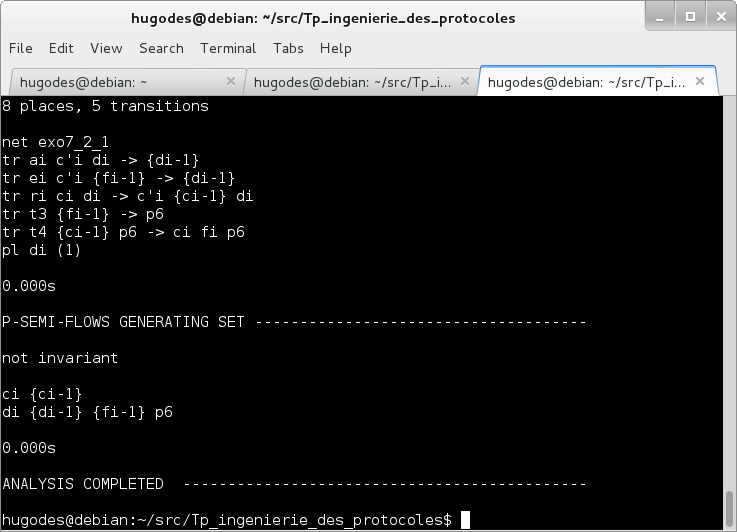
\includegraphics[width=0.7\textwidth]{exo7/tina_7_2.png}\\

\end{center}

On va utiliser l'algorithme de Farkas pour calculer les P-semi flots du second schéma.

\begin{center}


{\Huge C}\qquad =\qquad $\bordermatrix{
&ai&ei&ri&t1&t2\cr
ci&0&0&-1&0&1\cr
c'i&-1&-1&1&0&0\cr
ci-1&0&0&1&0&-1\cr
di&-1&0&0&0&0\cr
di-1&1&1&0&0&0\cr
fi-1&0&-1&0&-1&0\cr
fi&0&0&0&0&1\cr
p1&0&0&0&1&0\cr
}$

{\Huge $\downarrow$}

$\bordermatrix{
&ei&ri&t1&t2\cr
ci&0&-1&0&1\cr
c'i+di-1&0&1&0&0\cr
ci-1&0&1&0&-1\cr
di+di-1&1&0&0&0\cr
fi-1&-1&0&-1&0\cr
fi&0&0&0&1\cr
p1&0&0&1&0\cr
}$

{\Huge $\downarrow$}

$\bordermatrix{
&ri&t1&t2\cr
ci&-1&0&1\cr
c'i+di-1&1&0&0\cr
ci-1&1&0&-1\cr
di+di-1+fi-1&0&-1&0\cr
fi&0&0&1\cr
p1&0&1&0\cr
}$

{\Huge $\downarrow$}

$\bordermatrix{
&t1&t2\cr
c'i+di-1+ci&0&1\cr
ci-1+ci&0&0\cr
di+di-1+fi-1&-1&0\cr
fi&0&1\cr
p1&1&0\cr
}$

{\Huge $\downarrow$}

$\bordermatrix{
&t2\cr
c'i+di-1+ci&1\cr
di+di-1+fi-1+p1&0\cr
fi&1\cr
}$

\vspace{1cm}

On trouve donc 2 P-semi flots :\\
$f_1 = (0\ 1\ 1\ 0\ 0\ 0\ 0\ 0)$\\
$f_2 = (0\ 0\ 1\ 1\ 1\ 0\ 0\ 1)$\\

\end{center}

On obtient donc le même résultat que TINA.


\subsection{Question 2}
\subsubsection{Question 2.1}
Pour le premier schéma la séquence maximale est:\\
t1 -> n*t4 -> t2 -> 2n*t5 -> t3 

\subsubsection{Question 2.2}
Pour le second schéma la séquence maximale est:\\
t1 -> n*t4 -> t2 -> 2n*t5 -> t3 

\section{Exercice 8 - Spécification d'une construction d'une maison}
\subsection{Question 1}
 Le protocole peut être décrit par le réseau suivant : \\

\begin{figure}[H]
  \centering
  \begin{tikzpicture}

    % Liste des places
    \draw (0,8) node[below right = 2pt] {$P_1$};
    \node[draw,circle,scale=2] (P1) at (0, 8) {};
    \draw (0,4) node[below right = 2pt] {$P_2$};
    \node[draw,circle,scale=2] (P2) at (0,4) {};
    \draw (0,0) node[below right = 2pt] {$P_3$};
    \node[draw,circle,scale=2] (P3) at (0, 0) {};
    \draw (-2,-4) node[below right = 2pt] {$P_4$};
    \node[draw,circle,scale=2] (P4) at (-2,-4) {};
    \draw (-2,-8) node[below right = 2pt] {$P_5$};
    \node[draw,circle,scale=2] (P5) at (-2, -8) {};
     \draw (2,-4) node[below right = 2pt] {$P_6$};
    \node[draw,circle,scale=2] (P6) at (2, -4) {};
    \draw (2,-8) node[below right = 2pt] {$P_7$};
    \node[draw,circle,scale=2] (P7) at (2,-8) {};
    \draw (4,-8) node[below right = 2pt] {$P_8$};
    \node[draw,circle,scale=2] (P8) at (4, -8) {};
    \draw (2,-12) node[below right = 2pt] {$P_9$};
    \node[draw,circle,scale=2] (P9) at (2,-12) {};

     % Liste des transitions
    \draw (0,10) node[below = 10pt] {$t_1$};
    \node[draw,rectangle,yscale=4] (t1) at (0, 10) {};
    \draw (0,6) node[below right = 4pt] {$t_2$};
    \node[draw,rectangle,yscale=4] (t2) at (0, 6) {};
    \draw (0,2) node[below right= 4pt] {$t_3$};
    \node[draw,rectangle,yscale=4] (t3) at (0, 2) {};
    \draw (-2,-2) node[below = 10pt] {$t_4$};
    \node[draw,rectangle,yscale=4] (t4) at (-2, -2) {};
    \draw (-2,-6) node[below = 10pt] {$t_5$};
    \node[draw,rectangle,yscale=4] (t5) at (-2, -6) {};
    \draw (2,-2) node[below right = 3pt] {$t_6$};
    \node[draw,rectangle,yscale=4] (t6) at (2, -2) {};
    \draw (2,-6) node[below right = 3pt] {$t_7$};
    \node[draw,rectangle,yscale=4] (t7) at (2, -6) {};
    \draw (4,-6) node[below right = 3pt] {$t_8$};
    \node[draw,rectangle,yscale=4] (t8) at (4, -6) {};
    \draw (2,-10) node[below right = 3pt] {$t_9$};
    \node[draw,rectangle,yscale=4] (t9) at (2, -10) {};
    \draw (2,-14) node[below right = 3pt] {$t_10$};
    \node[draw,rectangle,yscale=4] (t10) at (2, -14) {};

    % Liste des arcs
    \draw[->,>=latex] (t1) -- (P1);
    \draw[->,>=latex] (P1) -- (t2);
    \draw[->,>=latex] (t2) -- (P2);
    \draw[->,>=latex] (P2) -- (t3);
    \draw[->,>=latex] (t3) -- (P3);
    \draw[->,>=latex] (P3) -- (t4);
    \draw[->,>=latex] (t4) -- (P4);
    \draw[->,>=latex] (P4) -- (t5);
    \draw[->,>=latex] (t5) -- (P5);
    \draw[->,>=latex] (P5) -- (t10);
    \draw[->,>=latex] (P3) -- (t6);
    \draw[->,>=latex] (t6) -- (P6);
    \draw[->,>=latex] (P6) -- (t7);
    \draw[->,>=latex] (P6) -- (t8);
    \draw[->,>=latex] (t7) -- (P7);
    \draw[->,>=latex] (t8) -- (P8);
    \draw[->,>=latex] (P7) -- (t9);
    \draw[->,>=latex] (t9) -- (P9);
    \draw[->,>=latex] (P9) -- (t10);
    \draw[->,>=latex] (P8) -- (t10);


  \end{tikzpicture}
  \caption{Réseau de petri associé à l'exercice 8.1} \label{fig:M5}
\end{figure}

\subsection{Question 2}
 Le protocole peut être décrit par le réseau suivant : \\

\begin{figure}[H]
  \centering
  \begin{tikzpicture}

    % Liste des places
    \draw (0,10) node[below right = 2pt] {$P_1$};
    \node[draw,circle,scale=2] (P1) at (0, 10) {};
    \draw (0,6) node[below right = 2pt] {$P_2$};
    \node[draw,circle,scale=2] (P2) at (0,6) {};
    \draw (0,2) node[below right = 2pt] {$P_3$};
    \node[draw,circle,scale=2] (P3) at (0, 2) {};
    \draw (-2,-2) node[below right = 2pt] {$P_4$};
    \node[draw,circle,scale=2] (P4) at (-2,-2) {};
    \draw (-2,-6) node[below right = 2pt] {$P_5$};
    \node[draw,circle,scale=2] (P5) at (-2, -6) {};
     \draw (2,-2) node[below right = 2pt] {$P_6$};
    \node[draw,circle,scale=2] (P6) at (2, -2) {};
    \draw (2,-6) node[below right = 2pt] {$P_7$};
    \node[draw,circle,scale=2] (P7) at (2,-6) {};
    \draw (4,-6) node[below right = 2pt] {$P_8$};
    \node[draw,circle,scale=2] (P8) at (4, -6) {};
    \draw (2,-10) node[below right = 2pt] {$P_9$};
    \node[draw,circle,scale=2] (P9) at (2,-10) {};
    \draw (2,-14) node[below right = 2pt] {$P_10$};
    \node[draw,circle,scale=2] (P10) at (2,-14) {};

     % Liste des transitions
    \draw (0,8) node[below = 10pt] {$t_1$};
    \node[draw,rectangle,yscale=4] (t1) at (0, 8) {};
    \draw (0,4) node[below right = 4pt] {$t_2$};
    \node[draw,rectangle,yscale=4] (t2) at (0, 4) {};
    \draw (-2,0) node[below right= 4pt] {$t_3$};
    \node[draw,rectangle,yscale=4] (t3) at (-2, 0) {};
    \draw (-2,-4) node[below = 10pt] {$t_4$};
    \node[draw,rectangle,yscale=4] (t4) at (-2, -4) {};
    \draw (-2,-8) node[below = 10pt] {$t_5$};
    \node[draw,rectangle,yscale=4] (t5) at (-2, -8) {};
    \draw (2,0) node[below right = 3pt] {$t_6$};
    \node[draw,rectangle,yscale=4] (t6) at (2, 0) {};
    \draw (2,-4) node[below right = 3pt] {$t_7$};
    \node[draw,rectangle,yscale=4] (t7) at (2, -4) {};
    \draw (4,-4) node[below right = 3pt] {$t_8$};
    \node[draw,rectangle,yscale=4] (t8) at (4, -4) {};
    \draw (2,-8) node[below right = 3pt] {$t_9$};
    \node[draw,rectangle,yscale=4] (t9) at (2, -8) {};
    \draw (4,-8) node[below right = 3pt] {$t_10$};
    \node[draw,rectangle,yscale=4] (t10) at (4, -8) {};
    \draw (2,-12) node[below right = 3pt] {$t_11$};
    \node[draw,rectangle,yscale=4] (t11) at (2, -12) {};

     % Liste des arcs
    \draw[->,>=latex] (P1) -- (t1);
    \draw[->,>=latex] (t1) -- (P2);
    \draw[->,>=latex] (P2) -- (t2);
    \draw[->,>=latex] (t2) -- (P3);
    \draw[->,>=latex] (P3) -- (t3);
    \draw[->,>=latex] (t3) -- (P4);
    \draw[->,>=latex] (P4) -- (t4);
    \draw[->,>=latex] (t4) -- (P5);
    \draw[->,>=latex] (P5) -- (t5);
    \draw[->,>=latex] (t5) -- (P10);
    \draw[->,>=latex] (P3) -- (t6);
    \draw[->,>=latex] (t6) -- (P6);
    \draw[->,>=latex] (P6) -- (t7);
    \draw[->,>=latex] (P6) -- (t8);
    \draw[->,>=latex] (t7) -- (P7);
    \draw[->,>=latex] (t8) -- (P8);
    \draw[->,>=latex] (P7) -- (t9);
    \draw[->,>=latex] (t9) -- (P9);
    \draw[->,>=latex] (P9) -- (t11);
    \draw[->,>=latex] (t11) -- (P10);
    \draw[->,>=latex] (P8) -- (t10);
    \draw[->,>=latex] (t10) -- (P10);




  \end{tikzpicture}
  \caption{Réseau de petri associé à l'exercice 8.2} \label{fig:M5}
\end{figure}
\section{Exercice 9 - Producers and Consumers}
\subsection{Question 1}
En mettant $p$ jetons dans la place $Producer$, on représente $p$ producteurs qui vont pouvoir créer leur produit en parallèle.
En effet, chaque jeton consommé par la transition $Produce$ dans $Producer$ représente l'action d'un producteur qui pourra se produire un autre objet lorsque son jeton sera revenu en $Producer$, c'est à dire quand son produit sera fini et envoyé.
De même, en mettant $c$ jetons en place $Consumer$, on représente la présence de $c$ clients qui peuvent receptionner un seul produit à la fois.

\begin{figure}[H]
  \centering
  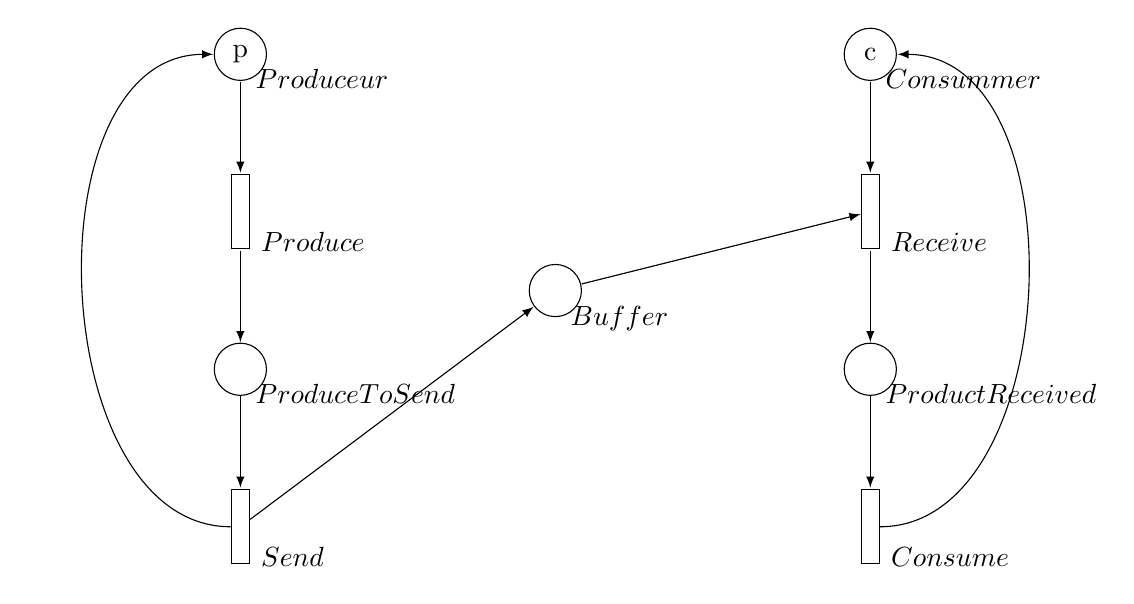
\begin{tikzpicture}

  	% Liste des places
    \draw (-4,3) node[below right = 2pt] {$Produceur$};
    \node[draw,circle,scale=2] (P) at (-4, 3) {};
    \draw (4,3) node[below right = 2pt] {$Consummer$};
    \node[draw,circle,scale=2] (C) at (4, 3) {};
    \draw (-4,-1) node[below right = 2pt] {$ProduceToSend$};
    \node[draw,circle,scale=2] (PtS) at (-4,-1) {};
    \draw (4,-1) node[below right = 2pt] {$ProductReceived$};
    \node[draw,circle,scale=2] (PR) at (4, -1) {}; %%
    \draw (0,0) node[below right = 2pt] {$Buffer$};
    \node[draw,circle,scale=2] (B) at (0, 0) {}; %%


     % Liste des transitions
    \draw (-4,1) node[below right = 4pt] {$Produce$};
    \node[draw,rectangle,yscale=4] (TP) at (-4, 1) {};
    \draw (-4,-3) node[below right = 4pt] {$Send$};
    \node[draw,rectangle,yscale=4] (TS) at (-4, -3) {};
    \draw (4,1) node[below right= 4pt] {$Receive$};
    \node[draw,rectangle,yscale=4] (TR) at (4, 1) {};
    \draw (4,-3) node[below right = 4pt] {$Consume$};
    \node[draw,rectangle,yscale=4] (TC) at (4, -3) {};

     % Liste des arcs
    \draw[->,>=latex] (P) -- (TP);
    \draw[->,>=latex] (TP) -- (PtS);
    \draw[->,>=latex] (PtS) -- (TS);
    \draw[->,>=latex] (TS) -- (B);
    \draw[->,>=latex] (B) -- (TR);
    \draw[->,>=latex] (TS) to [out=180,in=180] (P);
    \draw[->,>=latex] (C) -- (TR);
    \draw[->,>=latex] (TR) -- (PR);
    \draw[->,>=latex] (PR) -- (TC);
    \draw[->,>=latex] (TC) to [out=0,in=0] (C);

    % Marquage
    \node (p) at (-4,3) {p};
    \node (c) at (4,3) {c};

    \end{tikzpicture}
  \caption{Réseau de petri associé à l'exercice 9.1} \label{fig:M5}
\end{figure}

\subsection{Question 2}
En rajoutant une place $Borne$ qui sera rempli par la senbilisation de $Receive$ et vider par celle de $Send$, on limite le nombre de message envoyé et donc le nombre de jeton dans la place $Buffer$.

\begin{figure}[H]
  \centering
  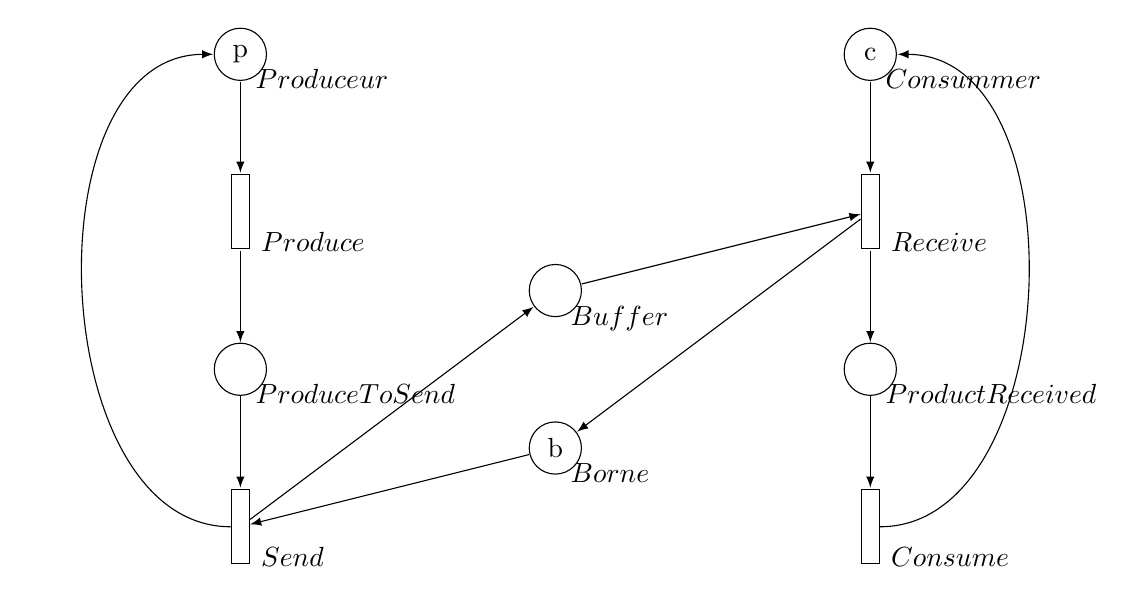
\begin{tikzpicture}

  	% Liste des places
    \draw (-4,3) node[below right = 2pt] {$Produceur$};
    \node[draw,circle,scale=2] (P) at (-4, 3) {};
    \draw (4,3) node[below right = 2pt] {$Consummer$};
    \node[draw,circle,scale=2] (C) at (4, 3) {};
    \draw (-4,-1) node[below right = 2pt] {$ProduceToSend$};
    \node[draw,circle,scale=2] (PtS) at (-4,-1) {};
    \draw (4,-1) node[below right = 2pt] {$ProductReceived$};
    \node[draw,circle,scale=2] (PR) at (4, -1) {}; 
    \draw (0,0) node[below right = 2pt] {$Buffer$};
    \node[draw,circle,scale=2] (B) at (0, 0) {}; 
    \draw (0,-2) node[below right = 2pt] {$Borne$};
    \node[draw,circle,scale=2] (Br) at (0, -2) {}; 


     % Liste des transitions
    \draw (-4,1) node[below right = 4pt] {$Produce$};
    \node[draw,rectangle,yscale=4] (TP) at (-4, 1) {};
    \draw (-4,-3) node[below right = 4pt] {$Send$};
    \node[draw,rectangle,yscale=4] (TS) at (-4, -3) {};
    \draw (4,1) node[below right= 4pt] {$Receive$};
    \node[draw,rectangle,yscale=4] (TR) at (4, 1) {};
    \draw (4,-3) node[below right = 4pt] {$Consume$};
    \node[draw,rectangle,yscale=4] (TC) at (4, -3) {};

     % Liste des arcs
    \draw[->,>=latex] (P) -- (TP);
    \draw[->,>=latex] (TP) -- (PtS);
    \draw[->,>=latex] (PtS) -- (TS);
    \draw[->,>=latex] (TS) -- (B);
    \draw[->,>=latex] (B) -- (TR);
    \draw[->,>=latex] (TS) to [out=180,in=180] (P);
    \draw[->,>=latex] (C) -- (TR);
    \draw[->,>=latex] (TR) -- (PR);
    \draw[->,>=latex] (PR) -- (TC);
    \draw[->,>=latex] (TC) to [out=0,in=0] (C);
    \draw[->,>=latex] (TR) -- (Br);
    \draw[->,>=latex] (Br) -- (TS);

    % Marquage
    \node (p) at (-4,3) {p};
    \node (c) at (4,3) {c};
    \node (b) at (0,-2) {b};

    \end{tikzpicture}
  \caption{Réseau de petri associé à l'exercice 9.2} \label{fig:M5}
\end{figure}

\subsection{Question 3}
En limitant le marquage de la place $Borne$ à une unité, on s'assure qu'un message ne sera envoyé que lorsque le précédant aura été reçu.
Ainsi il sont forcément reçu dans l'ordre d'envoie.

\begin{figure}[H]
  \centering
  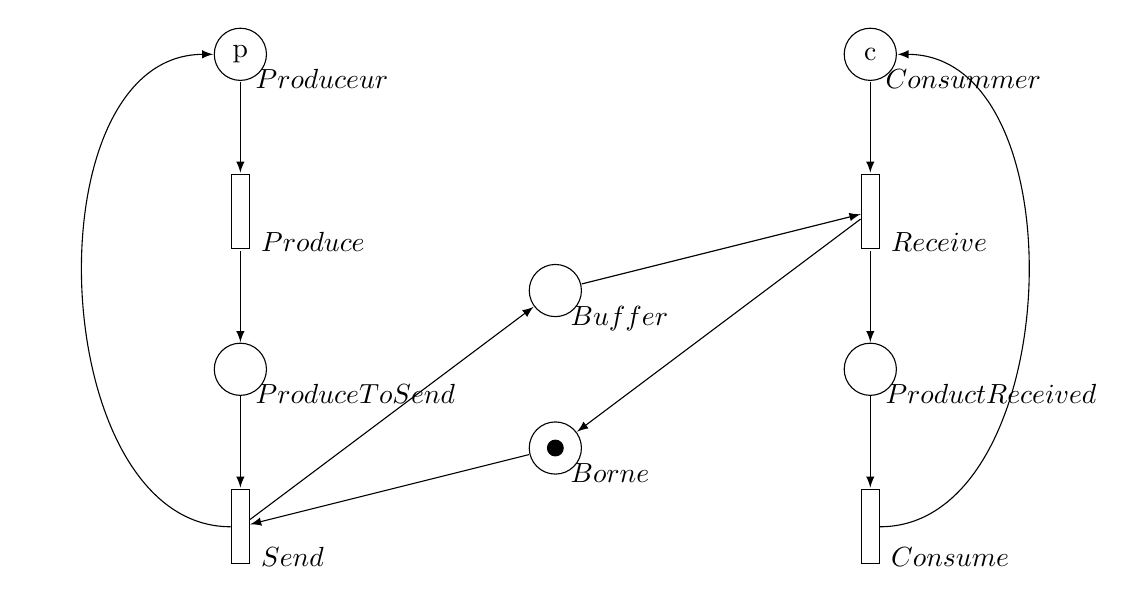
\begin{tikzpicture}

  	% Liste des places
    \draw (-4,3) node[below right = 2pt] {$Produceur$};
    \node[draw,circle,scale=2] (P) at (-4, 3) {};
    \draw (4,3) node[below right = 2pt] {$Consummer$};
    \node[draw,circle,scale=2] (C) at (4, 3) {};
    \draw (-4,-1) node[below right = 2pt] {$ProduceToSend$};
    \node[draw,circle,scale=2] (PtS) at (-4,-1) {};
    \draw (4,-1) node[below right = 2pt] {$ProductReceived$};
    \node[draw,circle,scale=2] (PR) at (4, -1) {}; 
    \draw (0,0) node[below right = 2pt] {$Buffer$};
    \node[draw,circle,scale=2] (B) at (0, 0) {}; 
    \draw (0,-2) node[below right = 2pt] {$Borne$};
    \node[draw,circle,scale=2] (Br) at (0, -2) {}; 


     % Liste des transitions
    \draw (-4,1) node[below right = 4pt] {$Produce$};
    \node[draw,rectangle,yscale=4] (TP) at (-4, 1) {};
    \draw (-4,-3) node[below right = 4pt] {$Send$};
    \node[draw,rectangle,yscale=4] (TS) at (-4, -3) {};
    \draw (4,1) node[below right= 4pt] {$Receive$};
    \node[draw,rectangle,yscale=4] (TR) at (4, 1) {};
    \draw (4,-3) node[below right = 4pt] {$Consume$};
    \node[draw,rectangle,yscale=4] (TC) at (4, -3) {};

     % Liste des arcs
    \draw[->,>=latex] (P) -- (TP);
    \draw[->,>=latex] (TP) -- (PtS);
    \draw[->,>=latex] (PtS) -- (TS);
    \draw[->,>=latex] (TS) -- (B);
    \draw[->,>=latex] (B) -- (TR);
    \draw[->,>=latex] (TS) to [out=180,in=180] (P);
    \draw[->,>=latex] (C) -- (TR);
    \draw[->,>=latex] (TR) -- (PR);
    \draw[->,>=latex] (PR) -- (TC);
    \draw[->,>=latex] (TC) to [out=0,in=0] (C);
    \draw[->,>=latex] (TR) -- (Br);
    \draw[->,>=latex] (Br) -- (TS);

    % Marquage
    \node (p) at (-4,3) {p};
    \node (c) at (4,3) {c};
    \draw [fill](0,-2) circle (0.1);

    \end{tikzpicture}
  \caption{Réseau de petri associé à l'exercice 9.3} \label{fig:M5}
\end{figure}

\section{Exercice 10 - Producers and Consumers bis}
\subsection{Question 1}

\begin{figure}[H]
  \centering
  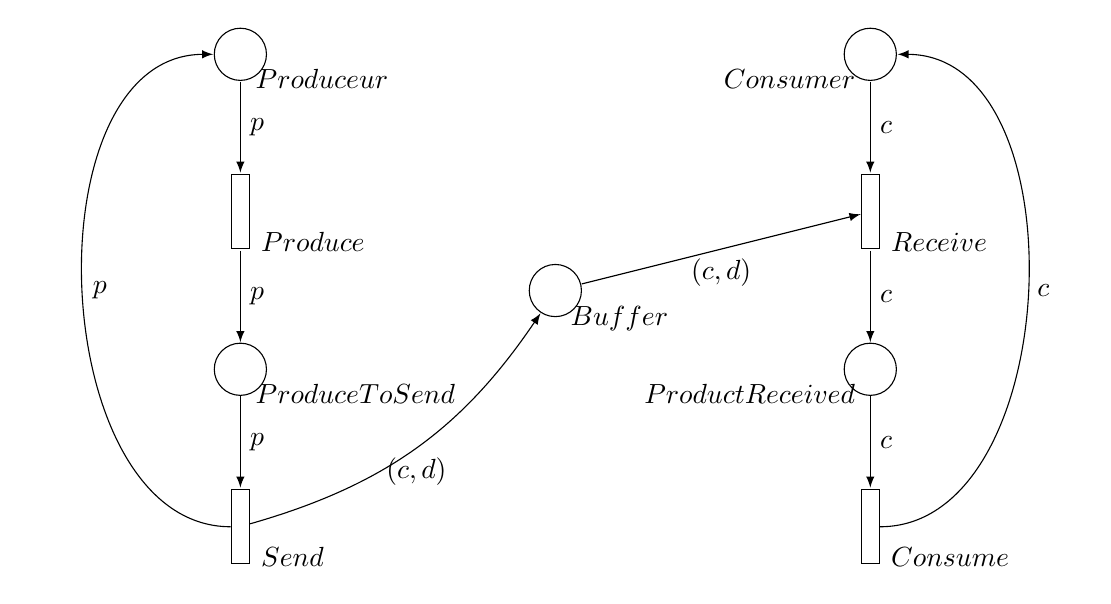
\begin{tikzpicture}

  	% Liste des places
    \draw (-4,3) node[below right = 2pt] {$Produceur$};
    \node[draw,circle,scale=2] (P) at (-4, 3) {};
    \draw (4,3) node[below left = 2pt] {$Consumer$};
    \node[draw,circle,scale=2] (C) at (4, 3) {};
    \draw (-4,-1) node[below right = 2pt] {$ProduceToSend$};
    \node[draw,circle,scale=2] (PtS) at (-4,-1) {};
    \draw (4,-1) node[below left = 2pt] {$ProductReceived$};
    \node[draw,circle,scale=2] (PR) at (4, -1) {}; %%
    \draw (0,0) node[below right = 2pt] {$Buffer$};
    \node[draw,circle,scale=2] (B) at (0, 0) {}; %%


     % Liste des transitions
    \draw (-4,1) node[below right = 4pt] {$Produce$};
    \node[draw,rectangle,yscale=4] (TP) at (-4, 1) {};
    \draw (-4,-3) node[below right = 4pt] {$Send$};
    \node[draw,rectangle,yscale=4] (TS) at (-4, -3) {};
    \draw (4,1) node[below right= 4pt] {$Receive$};
    \node[draw,rectangle,yscale=4] (TR) at (4, 1) {};
    \draw (4,-3) node[below right = 4pt] {$Consume$};
    \node[draw,rectangle,yscale=4] (TC) at (4, -3) {};

     % Liste des arcs
    \draw[->,>=latex] (P) -- (TP)node[midway, right]{$p$};
    \draw[->,>=latex] (TP) -- (PtS)node[midway, right]{$p$};
    \draw[->,>=latex] (PtS) -- (TS)node[midway, right]{$p$};
    \draw[->,>=latex] (TS) to[bend right = 20] node[midway, below]{$(c,d)$} (B);
    \draw[->,>=latex] (B) -- (TR)node[midway, below]{$(c,d)$};
    \draw[->,>=latex] (TS) to [out=180,in=180] node[midway, right]{$p$}(P);
    \draw[->,>=latex] (C) -- (TR)node[midway, right]{$c$};
    \draw[->,>=latex] (TR) -- (PR)node[midway, right]{$c$};
    \draw[->,>=latex] (PR) -- (TC)node[midway, right]{$c$};
    \draw[->,>=latex] (TC) to [out=0,in=0] node[midway, right]{$c$}(C);

    \end{tikzpicture}
  \caption{Réseau de petri coloré associé au protocole de production} \label{fig:M5}
\end{figure}

Lorsqu'un producteur crée un produit, un jeton avec une valeur $p$ est consommé en $Producer$ par $Produce$ et un jeton avec la même valeur est produit en $ProduceToSend$.
À ce moment là, la transition $Send$ consomme ce jeton de valeur $p$ en $ProduceToSend$ et va en produire 2, un dans $Producer$, avec la même valeur $p$,qui signifie que le producteur est à nouveau disponible, et un, en $Buffer$ avec un valeur double $(c,d)$ où $d$ correspond à la ``référence'' du produit et $c$ à son destinataire.
Ainsi, lorsque la transition $Receive$ sera sensibilisée, elle va associer le valeur $c$ du jeton $CONS$ consommé en $Consumer$ à la valeur $c$ contenu dans la paire du jeton $DATA$ consommé en $Buffer$.
Par conséquent, le reseau verifie que qu'un client consomme bien le produit qui lui est destiné.

\subsection{Question 2}

\begin{figure}[H]
  \centering
  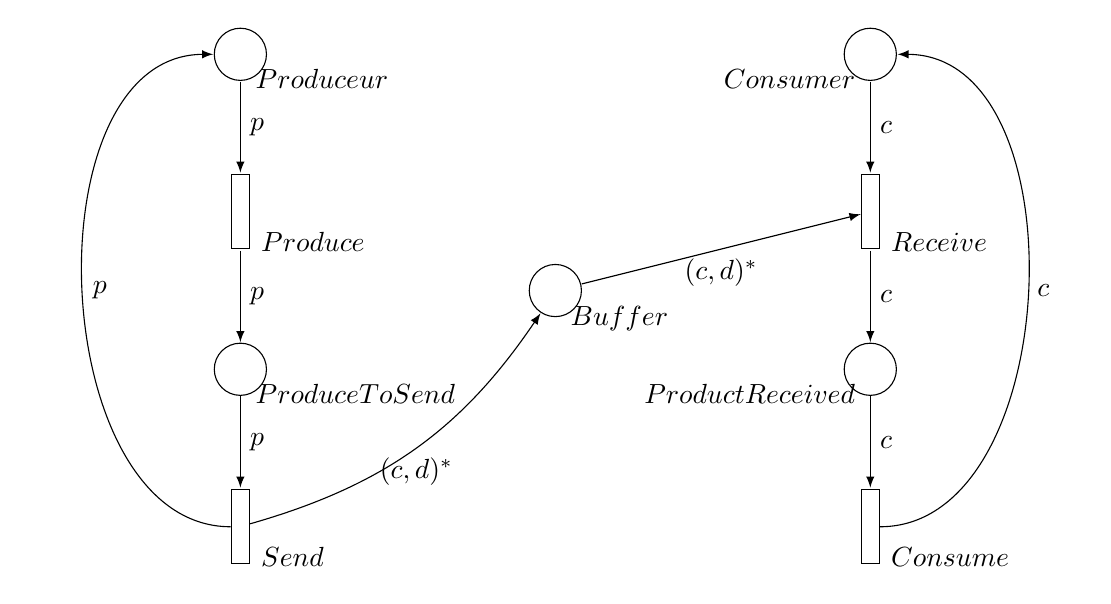
\begin{tikzpicture}

  	% Liste des places
    \draw (-4,3) node[below right = 2pt] {$Produceur$};
    \node[draw,circle,scale=2] (P) at (-4, 3) {};
    \draw (4,3) node[below left = 2pt] {$Consumer$};
    \node[draw,circle,scale=2] (C) at (4, 3) {};
    \draw (-4,-1) node[below right = 2pt] {$ProduceToSend$};
    \node[draw,circle,scale=2] (PtS) at (-4,-1) {};
    \draw (4,-1) node[below left = 2pt] {$ProductReceived$};
    \node[draw,circle,scale=2] (PR) at (4, -1) {}; %%
    \draw (0,0) node[below right = 2pt] {$Buffer$};
    \node[draw,circle,scale=2] (B) at (0, 0) {}; %%


     % Liste des transitions
    \draw (-4,1) node[below right = 4pt] {$Produce$};
    \node[draw,rectangle,yscale=4] (TP) at (-4, 1) {};
    \draw (-4,-3) node[below right = 4pt] {$Send$};
    \node[draw,rectangle,yscale=4] (TS) at (-4, -3) {};
    \draw (4,1) node[below right= 4pt] {$Receive$};
    \node[draw,rectangle,yscale=4] (TR) at (4, 1) {};
    \draw (4,-3) node[below right = 4pt] {$Consume$};
    \node[draw,rectangle,yscale=4] (TC) at (4, -3) {};

     % Liste des arcs
    \draw[->,>=latex] (P) -- (TP)node[midway, right]{$p$};
    \draw[->,>=latex] (TP) -- (PtS)node[midway, right]{$p$};
    \draw[->,>=latex] (PtS) -- (TS)node[midway, right]{$p$};
    \draw[->,>=latex] (TS) to[bend right = 20] node[midway, below]{$(c,d)^*$} (B);
    \draw[->,>=latex] (B) -- (TR)node[midway, below]{$(c,d)^*$};
    \draw[->,>=latex] (TS) to [out=180,in=180] node[midway, right]{$p$}(P);
    \draw[->,>=latex] (C) -- (TR)node[midway, right]{$c$};
    \draw[->,>=latex] (TR) -- (PR)node[midway, right]{$c$};
    \draw[->,>=latex] (PR) -- (TC)node[midway, right]{$c$};
    \draw[->,>=latex] (TC) to [out=0,in=0] node[midway, right]{$c$}(C);

    \end{tikzpicture}
  \caption{Réseau de petri coloré associé au protocole de production} \label{fig:M5}
\end{figure}



Dans ce cas, la production de produits n'est pas modifiée, seul l'envoie change.
Lors de l'envoie des produits,il vont être rassembler dans un liste finie (type FIFO). Cette liste est alors envoyée et reçu sans modification.
Ainsi le premier élément qui devait être envoyé sera le premier à être mis dans la liste avant son envoie et également le premier à être pris dans la listeaprès sa réception.
Donc, grace à ce système, l'ordre d'envoie et de reception sont identique.

\section{Exercice 11 - Semaphore}
\subsection{Question 1}
\begin{enumerate}
\item Le reseau représentant une sémaphore
\begin{figure}[H]
  \centering
  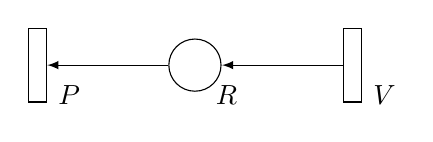
\begin{tikzpicture}
    % Liste des places
    \draw (0,0) node[below right = 4pt] {$R$};
    \node[draw,circle,scale=2] (R) at (0, 0) {};
    
      % Liste des transitions
    \draw (2,0) node[below right= 4pt] {$V$};
    \node[draw,rectangle,yscale=4] (V) at (2, 0) {};
    \draw (-2,0) node[below right= 4pt] {$P$};
    \node[draw,rectangle,yscale=4] (P) at (-2, 0) {};

     % Liste des arcs
    \draw[->,>=latex] (V) -- (R);
    \draw[->,>=latex] (R) -- (P);

  \end{tikzpicture}
  \caption{Réseau de petri associé à la sémaphore} \label{fig:M1}
\end{figure}


\item Simulation de l'évolution du réseau
Lorsqu'une ressource est mise à disposition, on a :

\begin{figure}[H]
  \centering
  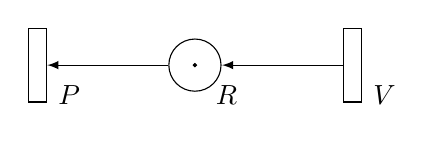
\begin{tikzpicture}
    % Liste des places
    \draw (0,0) node[below right = 4pt] {$R$};
    \node[draw,circle,scale=2] (R) at (0, 0) {};
    
      % Liste des transitions
    \draw (2,0) node[below right= 4pt] {$V$};
    \node[draw,rectangle,yscale=4] (V) at (2, 0) {};
    \draw (-2,0) node[below right= 4pt] {$P$};
    \node[draw,rectangle,yscale=4] (P) at (-2, 0) {};

     % Liste des arcs
    \draw[->,>=latex] (V) -- (R);
    \draw[->,>=latex] (R) -- (P);

     %Marquage
    \draw [fill](0,0) circle (0.02);

  \end{tikzpicture}
  \caption{Réseau de petri associé à la sémaphore} \label{fig:M1}
\end{figure}

On met à disposition une nouvelle ressource: 

\begin{figure}[H]
  \centering
  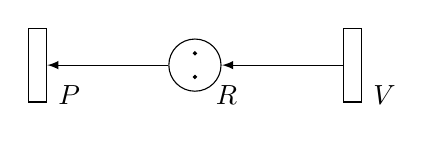
\begin{tikzpicture}
    % Liste des places
    \draw (0,0) node[below right = 4pt] {$R$};
    \node[draw,circle,scale=2] (R) at (0, 0) {};
    
      % Liste des transitions
    \draw (2,0) node[below right= 4pt] {$V$};
    \node[draw,rectangle,yscale=4] (V) at (2, 0) {};
    \draw (-2,0) node[below right= 4pt] {$P$};
    \node[draw,rectangle,yscale=4] (P) at (-2, 0) {};

     % Liste des arcs
    \draw[->,>=latex] (V) -- (R);
    \draw[->,>=latex] (R) -- (P);

     %Marquage
    \draw [fill](0,0.15) circle (0.02);
    \draw [fill](0,-0.15) circle (0.02);

  \end{tikzpicture}
  \caption{Réseau de petri associé à la sémaphore} \label{fig:M1}
\end{figure}

Une ressource est monopolisée, on revient à la fig. 20\\
Et si on monopolise une nouvelle ressource on revient au graphe initial (fig. 19)\\
A ce moment, il est impossible d'acceder à une ressource tant qu'elle n'est pas mise à disposition comme vu précédemment.

\item Transitions concurente?

Dans le cas où le marquage de la place $R$ est non nul, les deux transitions peuvent être franchit indépendement.
Dans le cas ou le marquage de la place $R$ est nul, la transition $V$ peut être franchit, mais pas la transition P.
Cependant, l'incapacité de franchissement de P n'est pas du au franchissement de V.
Donc ces deux transition ne sont pas concurrentes.


\end{enumerate}



\section{Exercice 12 - L'utilisation des réseaux de Petri pour le contole des trains}
\subsection{Question 1}

\begin{figure}[H]
  \centering
  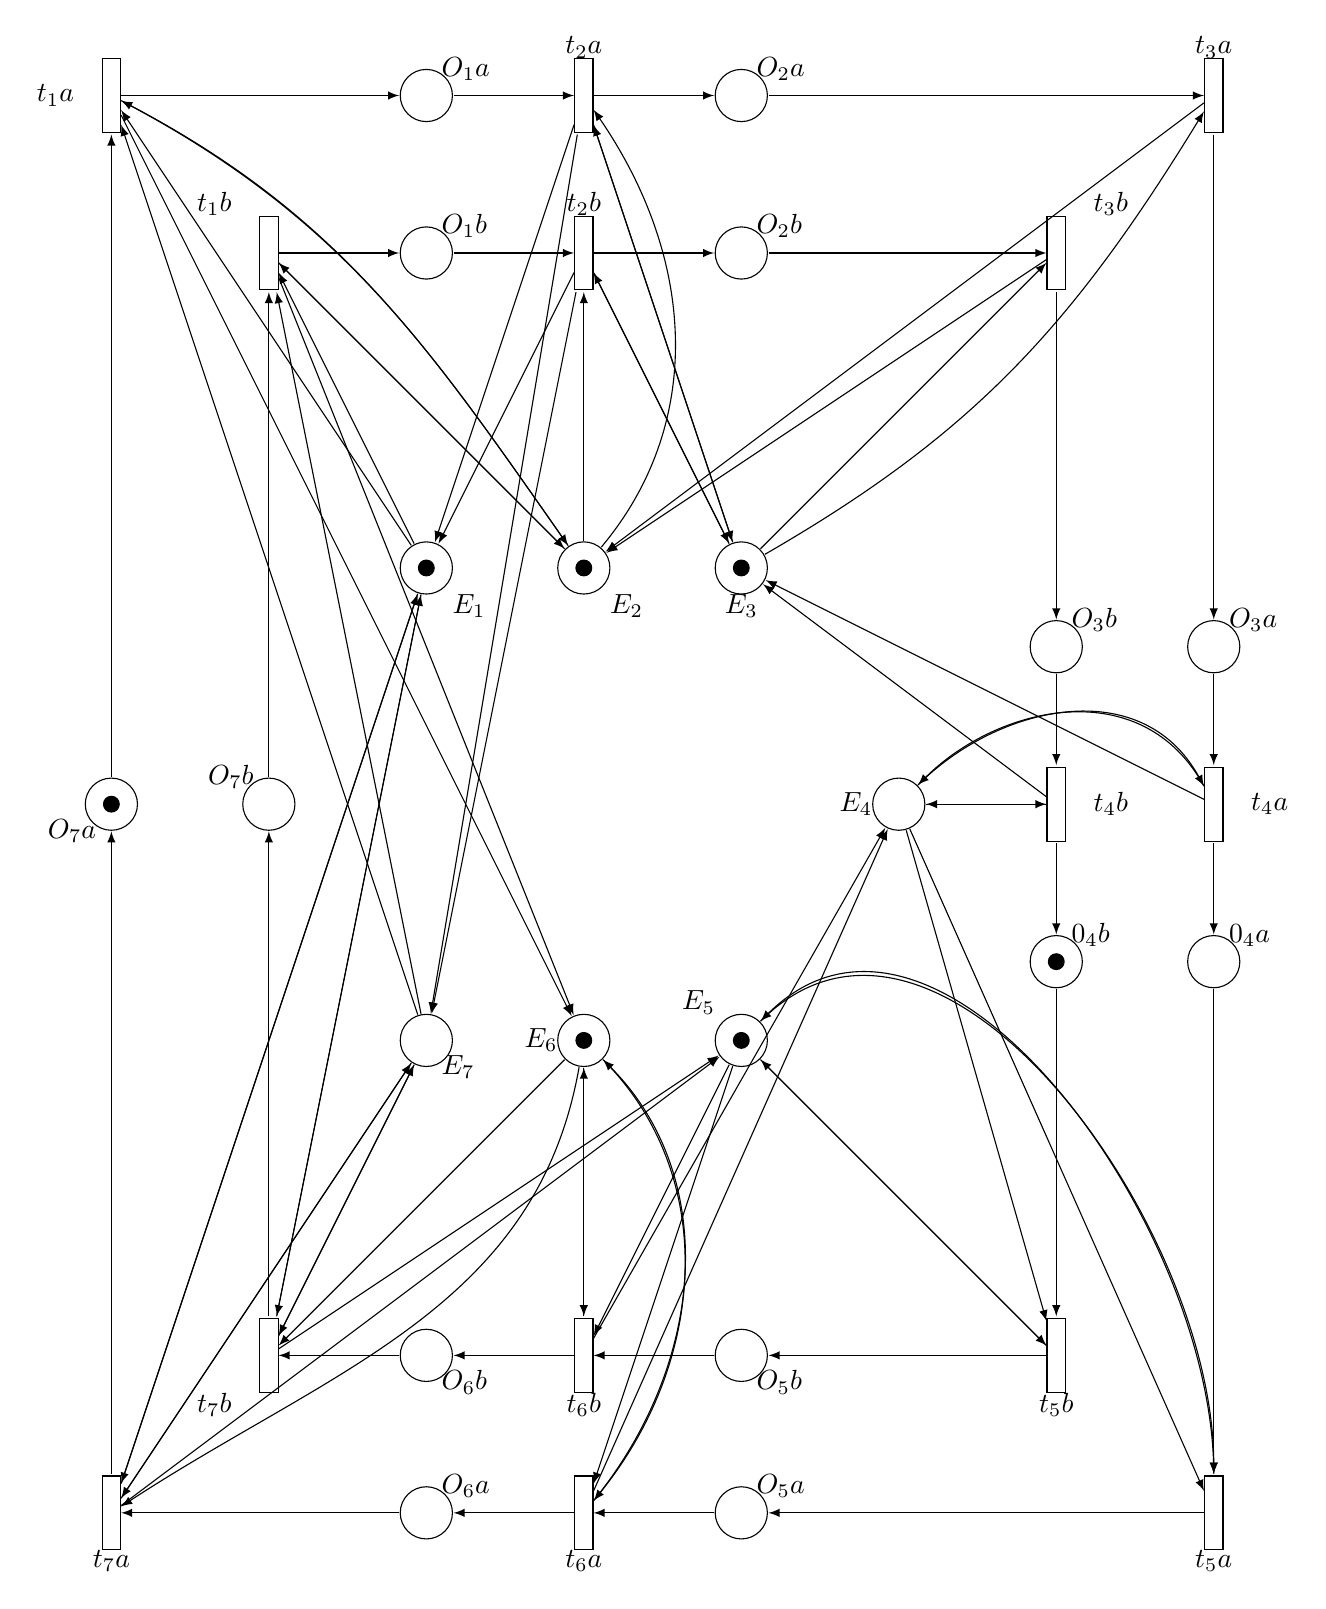
\begin{tikzpicture}
    % Liste des places
    \draw (-9,0) node[below left = 2pt] {$O_7a$};
    \node[draw,circle,scale=2] (o7a) at (-9, 0) {};

    \draw (-7,0) node[above left = 2pt] {$O_7b$};
    \node[draw,circle,scale=2] (o7b) at (-7, 0) {};

    \draw (-5, -7) node[below right = 2pt] {$O_6b$};
    \node[draw,circle,scale=2] (o6b) at (-5, -7) {};

    \draw (-5,-9) node[above right = 2pt] {$O_6a$};
    \node[draw,circle,scale=2] (o6a) at (-5, -9) {};

    \draw (-5,-3) node[below right = 2pt] {$E_7$};
    \node[draw,circle,scale=2] (e7) at (-5, -3) {};

    \draw (-5,3) node[below right = 6pt] {$E_1$};
    \node[draw,circle,scale=2] (e1) at (-5, 3) {};

    \draw (-5,7) node[above right = 2pt] {$O_1b$};
    \node[draw,circle,scale=2] (o1b) at (-5, 7) {};

    \draw (-5,9) node[above right = 2pt] {$O_1a$};
    \node[draw,circle,scale=2] (o1a) at (-5, 9) {};

    \draw (-3,3) node[below right = 6pt] {$E_2$};
    \node[draw,circle,scale=2] (e2) at (-3, 3) {};

    \draw (-3,-3) node[left = 6pt] {$E_6$};
    \node[draw,circle,scale=2] (e6) at (-3, -3) {};

    \draw (-1, -7) node[below right = 2pt] {$O_5b$};
    \node[draw,circle,scale=2] (o5b) at (-1, -7) {};

    \draw (-1,-9) node[above right = 2pt] {$O_5a$};
    \node[draw,circle,scale=2] (o5a) at (-1, -9) {};

    \draw (-1,-3) node[above left = 6pt] {$E_5$};
    \node[draw,circle,scale=2] (e5) at (-1, -3) {};

    \draw (-1,3) node[below = 6pt] {$E_3$};
    \node[draw,circle,scale=2] (e3) at (-1, 3) {};

    \draw (-1,7) node[above right = 2pt] {$O_2b$};
    \node[draw,circle,scale=2] (o2b) at (-1, 7) {};

    \draw (-1,9) node[above right = 2pt] {$O_2a$};
    \node[draw,circle,scale=2] (o2a) at (-1, 9) {};

    \draw (1,0) node[left = 6pt] {$E_4$};
    \node[draw,circle,scale=2] (e4) at (1, 0) {};

    \draw (3,2) node[above right = 2pt] {$O_3b$};
    \node[draw,circle,scale=2] (o3b) at (3, 2) {};

    \draw (3,-2) node[above right = 2pt] {$0_4b$};
    \node[draw,circle,scale=2] (o4b) at (3, -2) {};

    \draw (5,2) node[above right = 2pt] {$O_3a$};
    \node[draw,circle,scale=2] (o3a) at (5, 2) {};

    \draw (5,-2) node[above right = 2pt] {$0_4a$};
    \node[draw,circle,scale=2] (o4a) at (5, -2) {};







    % Liste des transitions
    \draw (-9,9) node[left = 10pt] {$t_1a$};
    \node[draw,rectangle,yscale=4] (t1a) at (-9, 9) {};

    \draw (-7,7) node[above left = 10pt] {$t_1b$};
    \node[draw,rectangle,yscale=4] (t1b) at (-7, 7) {};

    \draw (-3,9) node[above = 10pt] {$t_2a$};
    \node[draw,rectangle,yscale=4] (t2a) at (-3, 9) {};

    \draw (-3,7) node[above = 10pt] {$t_2b$};
    \node[draw,rectangle,yscale=4] (t2b) at (-3, 7) {};

    \draw (5,9) node[above = 10pt] {$t_3a$};
    \node[draw,rectangle,yscale=4] (t3a) at (5, 9) {};

    \draw (3,7) node[above right = 10pt] {$t_3b$};
    \node[draw,rectangle,yscale=4] (t3b) at (3, 7) {};

    \draw (3,0) node[right = 10pt] {$t_4b$};
    \node[draw,rectangle,yscale=4] (t4b) at (3, 0) {};

    \draw (5,0) node[right = 10pt] {$t_4a$};
    \node[draw,rectangle,yscale=4] (t4a) at (5, 0) {};

    \draw (5,-9) node[below = 10pt] {$t_5a$};
    \node[draw,rectangle,yscale=4] (t5a) at (5, -9) {};

    \draw (3,-7) node[below = 10pt] {$t_5b$};
    \node[draw,rectangle,yscale=4] (t5b) at (3, -7) {};

    \draw (-3,-9) node[below = 10pt] {$t_6a$};
    \node[draw,rectangle,yscale=4] (t6a) at (-3, -9) {};

    \draw (-3, -7) node[below = 10pt] {$t_6b$};
    \node[draw,rectangle,yscale=4] (t6b) at (-3, -7) {};

    \draw (-9,-9) node[below = 10pt] {$t_7a$};
    \node[draw,rectangle,yscale=4] (t7a) at (-9, -9) {};

    \draw (-7,-7) node[below left = 10pt] {$t_7b$};
    \node[draw,rectangle,yscale=4] (t7b) at (-7, -7) {};



    % Liste des arcs
    \draw[->,>=latex] (t1a) -- (o1a);

    \draw[->,>=latex] (o1a) -- (t2a);

    \draw[->,>=latex] (t2a) -- (o2a);

    \draw[->,>=latex] (o2a) -- (t3a);

    \draw[->,>=latex] (t3a) -- (o3a);

    \draw[->,>=latex] (o3a) -- (t4a);

    \draw[->,>=latex] (t4a) -- (o4a);

    \draw[->,>=latex] (o4a) -- (t5a);

    \draw[->,>=latex] (t5a) -- (o5a);

    \draw[->,>=latex] (o5a) -- (t6a);

    \draw[->,>=latex] (t6a) -- (o6a);

    \draw[->,>=latex] (o6a) -- (t7a);

    \draw[->,>=latex] (t7a) -- (o7a);

    \draw[->,>=latex] (o7a) -- (t1a);



    \draw[->,>=latex] (t1b) -- (o1b);

    \draw[->,>=latex] (o1b) -- (t2b);

    \draw[->,>=latex] (t2b) -- (o2b);

    \draw[->,>=latex] (o2b) -- (t3b);

    \draw[->,>=latex] (t3b) -- (o3b);

    \draw[->,>=latex] (o3b) -- (t4b);

    \draw[->,>=latex] (t4b) -- (o4b);

    \draw[->,>=latex] (o4b) -- (t5b);

    \draw[->,>=latex] (t5b) -- (o5b);

    \draw[->,>=latex] (o5b) -- (t6b);

    \draw[->,>=latex] (t6b) -- (o6b);

    \draw[->,>=latex] (o6b) -- (t7b);

    \draw[->,>=latex] (t7b) -- (o7b);

    \draw[->,>=latex] (o7b) -- (t1b);



    \draw[->,>=latex] (e1) -- (t1b);

    \draw[->,>=latex] (e1) -- (t1a);

    \draw[->,>=latex] (e1) -- (t7a);

    \draw[->,>=latex] (e1) -- (t7b);

    \draw[->,>=latex] (t7a) -- (e1);

    \draw[->,>=latex] (t7b) -- (e1);

    \draw[->,>=latex] (t2a) -- (e1);

    \draw[->,>=latex] (t2b) -- (e1);


    \draw[->,>=latex] (e2) -- (t2b);

    \draw[->,>=latex] (e2) to[out=50,in=-50] (t2a);

    \draw[->,>=latex] (e2) to[out=125,in=-25] (t1a);

    \draw[->,>=latex] (e2) -- (t1b);

    \draw[->,>=latex] (t1a) to[out=-25,in=125] (e2);

    \draw[->,>=latex] (t1b) -- (e2);

    \draw[->,>=latex] (t3a) -- (e2);

    \draw[->,>=latex] (t3b) -- (e2);


    \draw[->,>=latex] (e3) -- (t3b);

    \draw[->,>=latex] (e3) to[out=30,in=-125] (t3a);

    \draw[->,>=latex] (e3) -- (t2a);

    \draw[->,>=latex] (e3) -- (t2b);

    \draw[->,>=latex] (t2a) -- (e3);

    \draw[->,>=latex] (t2b) -- (e3);

    \draw[->,>=latex] (t4a) -- (e3);

    \draw[->,>=latex] (t4b) -- (e3);


    \draw[->,>=latex] (e4) -- (t5b);

    \draw[->,>=latex] (e4) -- (t5a);

    \draw[->,>=latex] (e4) to[out=45,in=125] (t4a);

    \draw[->,>=latex] (e4) -- (t4b);

    \draw[->,>=latex] (t4a) to[out=125,in=45] (e4);

    \draw[->,>=latex] (t4b) -- (e4);

    \draw[->,>=latex] (t6a) -- (e4);

    \draw[->,>=latex] (t6b) -- (e4);


    \draw[->,>=latex] (e5) -- (t6b);

    \draw[->,>=latex] (e5) -- (t6a);

    \draw[->,>=latex] (e5) to[out=45,in=90] (t5a);

    \draw[->,>=latex] (e5) -- (t5b);

    \draw[->,>=latex] (t5a) to[out=90,in=45] (e5);

    \draw[->,>=latex] (t5b) -- (e5);

    \draw[->,>=latex] (t7a) -- (e5);

    \draw[->,>=latex] (t7b) -- (e5);


    \draw[->,>=latex] (e6) -- (t7b);

    \draw[->,>=latex] (e6) to[out=-100,in=30] (t7a);

    \draw[->,>=latex] (e6) to[out=-45,in=45] (t6a);

    \draw[->,>=latex] (e6) -- (t6b);

    \draw[->,>=latex] (t6a) to[out=45,in=-45] (e6);

    \draw[->,>=latex] (t6b) -- (e6);

    \draw[->,>=latex] (t1a) -- (e6);

    \draw[->,>=latex] (t1b) -- (e6);


    \draw[->,>=latex] (e7) -- (t1b);

    \draw[->,>=latex] (e7) -- (t1a);

    \draw[->,>=latex] (e7) -- (t7a);

    \draw[->,>=latex] (e7) -- (t7b);

    \draw[->,>=latex] (t7a) -- (e7);

    \draw[->,>=latex] (t7b) -- (e7);

    \draw[->,>=latex] (t2a) -- (e7);

    \draw[->,>=latex] (t2b) -- (e7);






    %\draw[->,>=latex] (po) to[out=135,in=-135] (t1);

    % Marquage
    \draw [fill](-5,3) circle (0.1) ;
    \draw [fill](-3,3) circle (0.1) ;
    \draw [fill](-3,-3) circle (0.1) ;
    \draw [fill](-1,-3) circle (0.1) ;
    \draw [fill](-1,3) circle (0.1) ;
    \draw [fill](3,-2) circle (0.1) ;
    \draw [fill](-9,0) circle (0.1) ;




  \end{tikzpicture}
    \caption{Rp de la question 12.1} \label{fig:M1}
\end{figure}

Un train ce trouvant dans la le secteur i voulant avancer, il faut que le secteur i+1 et i+2 soient libres.
Cela equivaux a actioner la transition ti+1, qui verifie que les places Ei+1 et Ei+2 contienent des jetons.
Ensuite, le secteur i est libéré, le secteur i+1 occupé et le secteur i+2 inchangé.
Cela equivaux a mettre un jeton dans la place Ei, enlever un jeton de la place Ei+1 et le rajouter dans $O_{a_i+1}$.
Pour continuer, le train doit verrifier que les secteurs i+2 et i+3 sont libres il libère alors i+1, i+2 devient occupé et i+3 reste inchangé.
Ce motif se reppete autant de fois que le train veux changer de secteur.

\subsection{Question 2}
\begin{figure}[H]
  \centering
  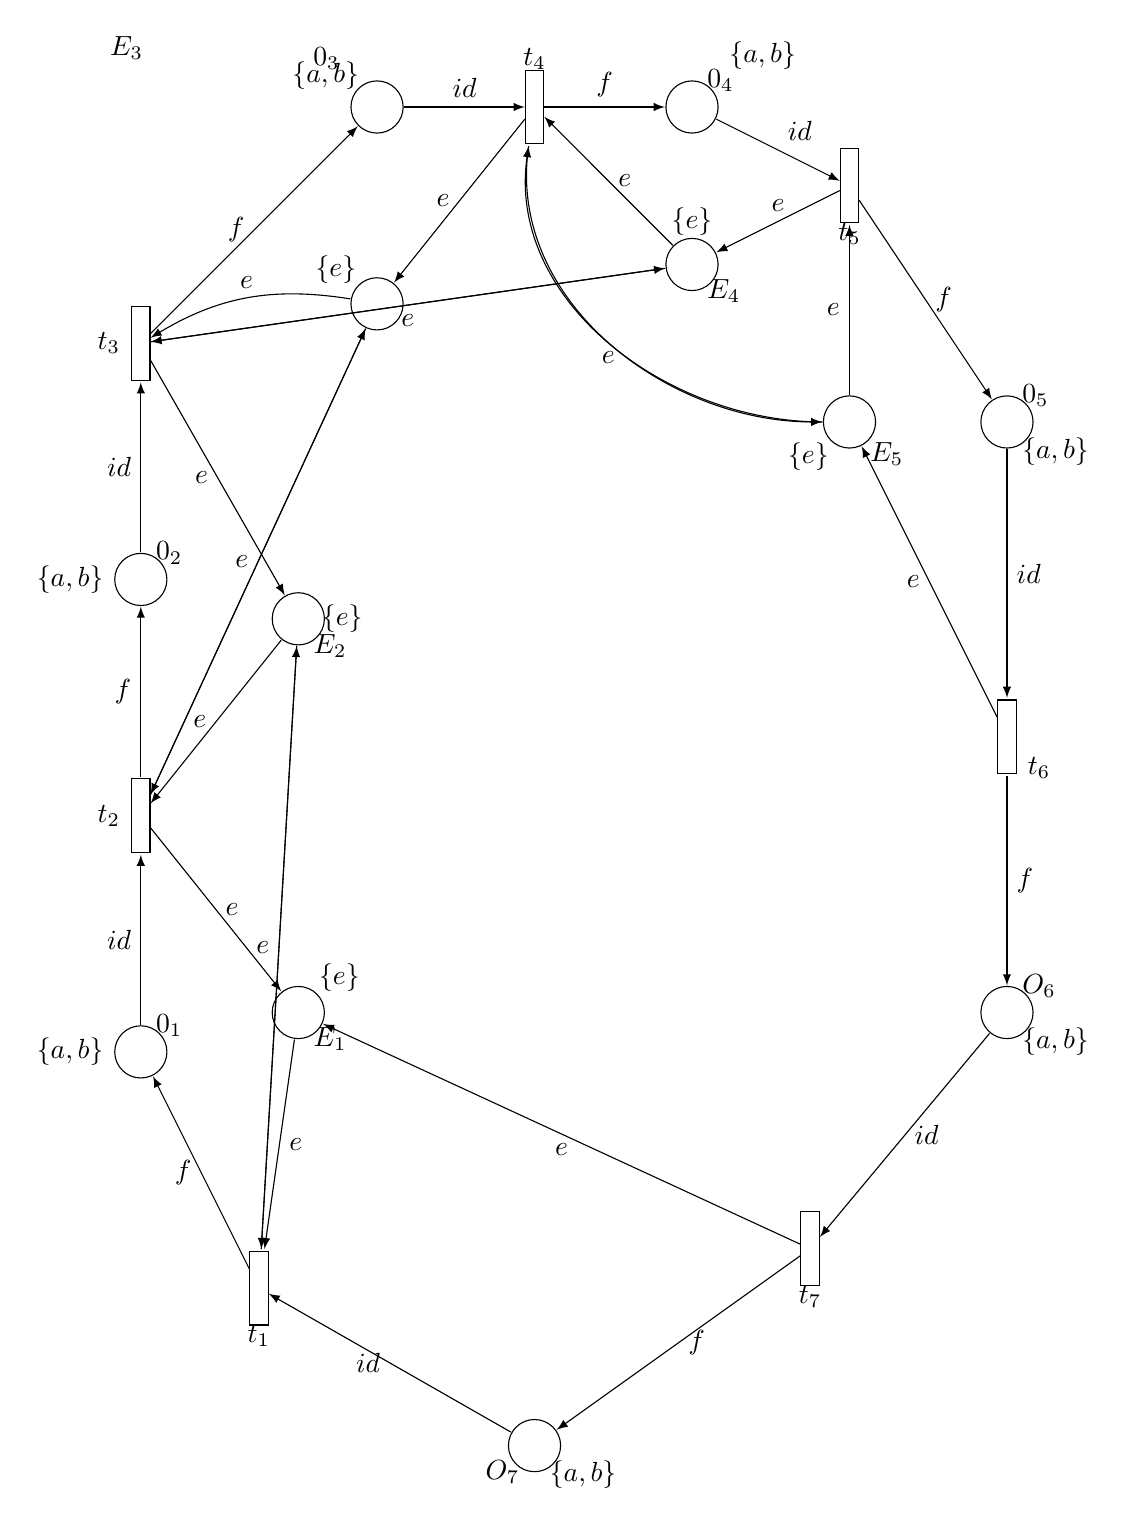
\begin{tikzpicture}

    % Liste des places
    \draw (0,-8) node[below left = 2pt] {$O_7$};
    \draw (0,-8) node[below right = 2pt] {$\{a,b\}$};
    \node[draw,circle,scale=2] (o7) at (0, -8) {};
    \draw (6,-2.5) node[above right = 2pt] {$O_6$};
    \draw (6,-2.5) node[below right = 2pt] {$\{a,b\}$};
    \node[draw,circle,scale=2] (o6) at (6, -2.5) {};
    \draw (6,5) node[above right = 2pt] {$0_5$};
    \draw (6,5) node[below right = 2pt] {$\{a,b\}$};
    \node[draw,circle,scale=2] (o5) at (6, 5) {};
    \draw (2,9) node[above right = 2pt] {$0_4$};
    \draw (2,9) node[above right = 10pt] {$\{a,b\}$};
    \node[draw,circle,scale=2] (o4) at (2, 9) {};
    \draw (-2,9) node[above left = 10pt] {$0_3$};
    \draw (-2,9) node[above left = 3pt] {$\{a,b\}$};
    \node[draw,circle,scale=2] (o3) at (-2, 9) {};
    \draw (-5,3) node[above right = 2pt] {$0_2$};
    \draw (-5,3) node[left = 10pt] {$\{a,b\}$};
    \node[draw,circle,scale=2] (o2) at (-5, 3) {};
    \draw (-5,-3) node[above right = 2pt] {$0_1$};
     \draw (-5,-3) node[left = 10pt] {$\{a,b\}$};
    \node[draw,circle,scale=2] (o1) at (-5, -3) {};
    \draw (-3,-2.5) node[below right = 2pt] {$E_1$};
    \draw (-3,-2.5) node[above right = 4pt] {$\{e\}$};
    \node[draw,circle,scale=2] (e1) at (-3, -2.5) {};
	\draw (-3,2.5) node[below right = 2pt] {$E_2$};
	\draw (-3,2.5) node[right = 5pt] {$\{e\}$};
    \node[draw,circle,scale=2] (e2) at (-3, 2.5) {};
    \draw (-2,6.5) node[below right = -100pt] {$E_3$};
    \draw (-2,6.5) node[above left = 4pt] {$\{e\}$};
    \node[draw,circle,scale=2] (e3) at (-2, 6.5) {};
    \draw (2, 7) node[below right = 2pt] {$E_4$};
    \draw (2,7) node[above = 7pt] {$\{e\}$};
    \node[draw,circle,scale=2] (e4) at (2, 7) {};
    \draw (4,5) node[below right = 4pt] {$E_5$};
    \draw (4,5) node[below left = 4pt] {$\{e\}$};
    \node[draw,circle,scale=2] (e5) at (4, 5) {};

    % Liste des transitions
    \draw (-3.5,-6) node[below = 10pt] {$t_1$};
    \node[draw,rectangle,yscale=4] (t1) at (-3.5, -6) {};
    \draw (-5,0) node[left = 4pt] {$t_2$};
    \node[draw,rectangle,yscale=4] (t2) at (-5, 0) {};
    \draw (-5,6) node[left = 4pt] {$t_3$};
    \node[draw,rectangle,yscale=4] (t3) at (-5, 6) {};
    \draw (0,9) node[above = 10pt] {$t_4$};
    \node[draw,rectangle,yscale=4] (t4) at (0, 9) {};
    \draw (4,8) node[below = 10pt] {$t_5$};
    \node[draw,rectangle,yscale=4] (t5) at (4, 8) {};
    \draw (6,1) node[below right = 4pt] {$t_6$};
    \node[draw,rectangle,yscale=4] (t6) at (6, 1) {};
    \draw (3.5,-5.5) node[below = 10pt] {$t_7$};
    \node[draw,rectangle,yscale=4] (t7) at (3.5, -5.5) {};

    % Liste des arcs
    \draw[->,>=latex] (o7) -- (t1) node[midway, left]{$id$};
    \draw[->,>=latex] (t1) -- (o1) node[midway, left]{$f$};
    \draw[->,>=latex] (o1) -- (t2) node[midway, left]{$id$};
    \draw[->,>=latex] (t2) -- (o2) node[midway, left]{$f$};
    \draw[->,>=latex] (o2) -- (t3) node[midway, left]{$id$};
    \draw[->,>=latex] (t3) -- (o3) node[midway, left]{$f$};
    \draw[->,>=latex] (o3) -- (t4) node[midway, above]{$id$};
    \draw[->,>=latex] (t4) -- (o4) node[midway, above]{$f$};
    \draw[->,>=latex] (o4) -- (t5) node[midway, above right]{$id$};
    \draw[->,>=latex] (t5) -- (o5) node[midway, right]{$f$};
    \draw[->,>=latex] (o5) -- (t6) node[midway, right]{$id$};
    \draw[->,>=latex] (t6) -- (o6) node[midway, right]{$f$};
    \draw[->,>=latex] (o6) -- (t7) node[midway, right]{$id$};
    \draw[->,>=latex] (t7) -- (o7) node[midway, right]{$f$};

    \draw[->,>=latex] (e1) -- (t1) node[midway, right]{$e$};
    \draw[->,>=latex] (t2) -- (e1) node[midway, right]{$e$};
    \draw[->,>=latex] (e2) -- (t1) node[midway, left]{$e$};
    \draw[->,>=latex] (t1) -- (e2);
    \draw[->,>=latex] (e3) -- (t2);
    \draw[->,>=latex] (t2) -- (e3) node[midway, left]{$e$};
    \draw[->,>=latex] (t3) -- (e2) node[midway, left]{$e$};
    \draw[->,>=latex] (e2) -- (t2) node[midway, left]{$e$};
    \draw[->,>=latex] (e3) to [bend right=20] node[midway, above]{$e$}(t3) ;
    \draw[->,>=latex] (t4) -- (e3) node[midway, left]{$e$};
    \draw[->,>=latex] (t3) -- (e4) node[midway, below]{$e$};
    \draw[->,>=latex] (e4) -- (t3);
    \draw[->,>=latex] (e4) -- (t4) node[midway, right]{$e$};
    \draw[->,>=latex] (t5) -- (e4) node[midway, above]{$e$};
    \draw[->,>=latex] (e5) to [out=-180, in=-100] node[midway, below]{$e$}(t4);
    \draw[->,>=latex] (t4) to [out=-100, in=-180] (e5);
    \draw[->,>=latex] (e5) -- (t5) node[midway, left]{$e$};
    \draw[->,>=latex] (t6) -- (e5) node[midway, left]{$e$};
    \draw[->,>=latex] (t7) -- (e1) node[midway, below]{$e$};



  \end{tikzpicture}
  \caption{Réseau de petri associé à 12.2} \label{fig:M1}
\end{figure}


\section{Exercice 13 - L'utilisation des réseaux de Petri pour le controle d'un système téléphonique}
\subsection{Question 13}
Le système téléphonique peut être modéliser de la manière suivante : \\

\begin{figure}[H]
  \centering
  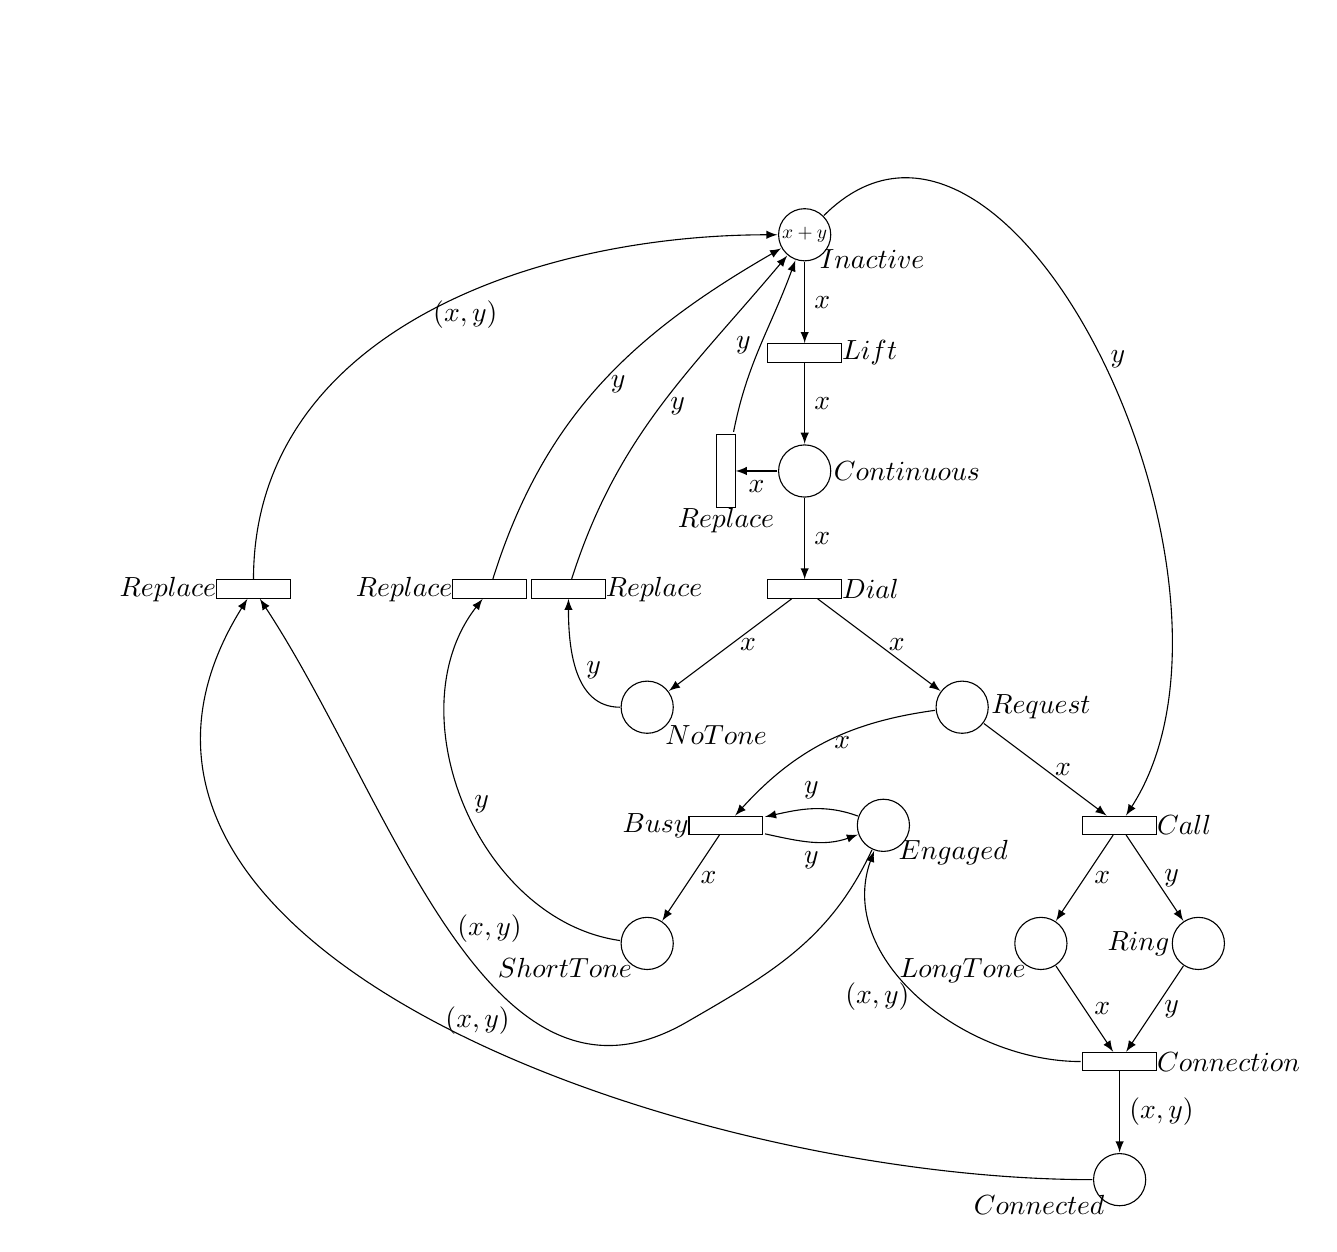
\begin{tikzpicture}
    % Liste des places
    \draw (0,8) node[below right = 2pt] {$Inactive$};
    \node[draw,circle,scale=2] (I) at (0, 8) {};
    \draw (0,5) node[right = 7pt] {$Continuous$};
    \node[draw,circle,scale=2] (C) at (0, 5) {};
    \draw (-2,2) node[below right = 3pt] {$No Tone$};
    \node[draw,circle,scale=2] (NT) at (-2,2) {};
    \draw (2,2) node[right = 7pt] {$Request$};
    \node[draw,circle,scale=2] (Re) at (2, 2) {};
    \draw (1,0.5) node[below right = 2pt] {$Engaged$};
    \node[draw,circle,scale=2] (E) at (1,0.5) {};
    \draw (-2,-1) node[below left = 2pt] {$Short Tone$};
    \node[draw,circle,scale=2] (ST) at (-2, -1) {};
    \draw (3,-1) node[below left = 2pt] {$Long Tone$};
    \node[draw,circle,scale=2] (LT) at (3,-1) {};
    \draw (5,-1) node[left = 7pt] {$Ring$};
    \node[draw,circle,scale=2] (Ri) at (5,-1) {};
    \draw (4,-4) node[below left = 2pt] {$Connected$};
    \node[draw,circle,scale=2] (Co) at (4,-4) {};

  % Liste des transitions
    \draw (0,6.5) node[right = 10pt] {$Lift$};
    \node[draw,rectangle,xscale=4] (L) at (0, 6.5) {};
    \draw (0,3.5) node[right = 10pt] {$Dial$};
    \node[draw,rectangle,xscale=4] (D) at (0, 3.5) {};
    \draw (-1,0.5) node[left = 10pt] {$Busy$};
    \node[draw,rectangle,xscale=4] (B) at (-1, 0.5) {};
    \draw (4,0.5) node[right = 10pt] {$Call$};
    \node[draw,rectangle,xscale=4] (Ca) at (4, 0.5) {};
    \draw (4,-2.5) node[right = 10pt] {$Connection$};
    \node[draw,rectangle,xscale=4] (TCo) at (4, -2.5) {};
    \draw (-1,5) node[below = 10pt] {$Replace$};
    \node[draw,rectangle,yscale=4] (R1) at (-1, 5) {};
    \draw (-3,3.5) node[right = 10pt] {$Replace$};
    \node[draw,rectangle,xscale=4] (R2) at (-3, 3.5) {};
    \draw (-4,3.5) node[left = 10pt] {$Replace$};
    \node[draw,rectangle,xscale=4] (R3) at (-4, 3.5) {};
    \draw (-7,3.5) node[left = 10pt] {$Replace$};
    \node[draw,rectangle,xscale=4] (R4) at (-7, 3.5) {};

  % Liste des arcs
    \draw[->,>=latex] (I) -- (L)node[midway, right]{$x$};
    \draw[->,>=latex] (L) -- (C)node[midway, right]{$x$};
    \draw[->,>=latex] (C) -- (R1)node[midway, below]{$x$};
    \draw[->,>=latex] (C) -- (D)node[midway, right]{$x$};
    \draw[->,>=latex] (D) -- (NT)node[midway, right]{$x$};
    \draw[->,>=latex] (D) -- (Re)node[midway, right]{$x$};
    \draw[->,>=latex] (Re) -- (Ca)node[midway, right]{$x$};
    \draw[->,>=latex] (Re) to[bend right=20] node[midway, right]{$x$} (B);
    \draw[->,>=latex] (Ca) -- (Ri)node[midway, right]{$y$};
    \draw[->,>=latex] (Ca) -- (LT)node[midway, right]{$x$};
    \draw[->,>=latex] (B) -- (ST)node[midway, right]{$x$};
    \draw[->,>=latex] (E) to[out=160, in=20] node[midway, above]{$y$} (B);
    \draw[->,>=latex] (B) to[out=-20,in=200] node[midway, below]{$y$} (E);
    \draw[->,>=latex] (LT) -- (TCo)node[midway, right]{$x$};
    \draw[->,>=latex] (Ri) -- (TCo)node[midway, right]{$y$};
    \draw[->,>=latex] (TCo) -- (Co)node[midway, right]{$(x,y)$};
    \draw[->,>=latex] (I) to[out=45,in=60] node[midway, right]{$y$}(Ca);
    \draw[->,>=latex] (R1) to[out=75,in=-110] node[midway, left]{$y$}(I);
    \draw[->,>=latex] (NT) to[out=180,in=-90] node[midway, right]{$y$}(R2);
    \draw[->,>=latex] (R2) to[out=75,in=-130] node[midway, right]{$y$}(I);
    \draw[->,>=latex] (ST) to[bend left=60] node[midway, right]{$y$}(R3);
    \draw[->,>=latex] (R3) to[out=75,in=-150] node[midway, right]{$y$}(I);
    \draw[->,>=latex] (TCo) to[out=180,in=-110] node[midway, left]{$(x,y)$}(E);
    \draw[->,>=latex] (Co) to[out=180,in=-120] node[midway, right]{$(x,y)$}(R4);
    \draw[->,>=latex] (R4) to[out=90,in=-180] node[midway, right]{$(x,y)$}(I);
    \draw[->,>=latex] (E) to[out=-115,in=30] (-1.5,-2) to[out=210,in=-60]  node[midway, right]{$(x,y)$}(R4);


    %Marquage
    \node(M0)[scale=0.7] at (0,8) {$x+y$};

  \end{tikzpicture}
  \caption{Réseau de petri associé au contrôle d'un système téléphonique} \label{fig:M1}
\end{figure}

\subsection{Question 2}

\begin{enumerate}
\item Evolution du sytème\\
Initialement, on considère que les deux téléphones sont inactifs.\\
on choisit arbitrairement la couleur $x$ pour désigner l'appelant et $y$ l'appelé.\\
Lorsque $x$ décroche sont téléphone(transition $Lift$), il entend une sonnerie continue représentée par la place $Continuous$.\\
À ce moment, $x$ peut soit raccrocher, $replace$, et redevenir inactif, soit composer un numéro, $Dial$ et attendre la réponse à sa demande, $Request$.\\
Si l'appelé $y$ est déjà en communication, $Engaged$, alors on sensibilise la transition $Busy$.\\
$y$ reste dans sa communication, $Engaged$, et $x$ recoit de courte sonnerie, $Short Tone$ avant de raccrocher, $replace$, et devenir inactive.\\
Si l'appelé $y$ est inactif, alors l'appel est envoyé, $Call$, et une longue sonnerie est envoyé à l'appelant, $x$ en $Long Tone$, et on fait sonner le téléphone de l'appelé, $y$ en $Ring$.\\
Lorsque l'appelé décroche, la connection s'établie entre les deux téléphones, $Connection$, et il sont en communication $Connected$.\\
Enfin, quand ils raccrochent, $replace$, ils redeviennent tous deux inactifs.

\item Cas particuliers
  \begin{itemize}
    \item Lorsque qu'un usager s'appele soit même, il va être engager dès qu'il va d'écrocher, donc il aura une sonnerie occupée. 
    \item Dans la modelisation que nous avons fait, la fin de connection peut être initier autant par l'appelant que par l'appelé.
    \item Avec nos maigre connaissance en téléphonie, il nous est difficile de dire avec certitude quel systême est utilisé en france.\\
Mais nous pensons que le modèle que nous avons fait peut correspondre au systême français.

  \end{itemize}
\end{enumerate}

\newpage

\section{Exercice 14 - Réseau de Petri temporel}
\subsection{Question 1}

Nous pouvons construire le graphe de classes suivant :

\begin{figure}[H]
  \centering
  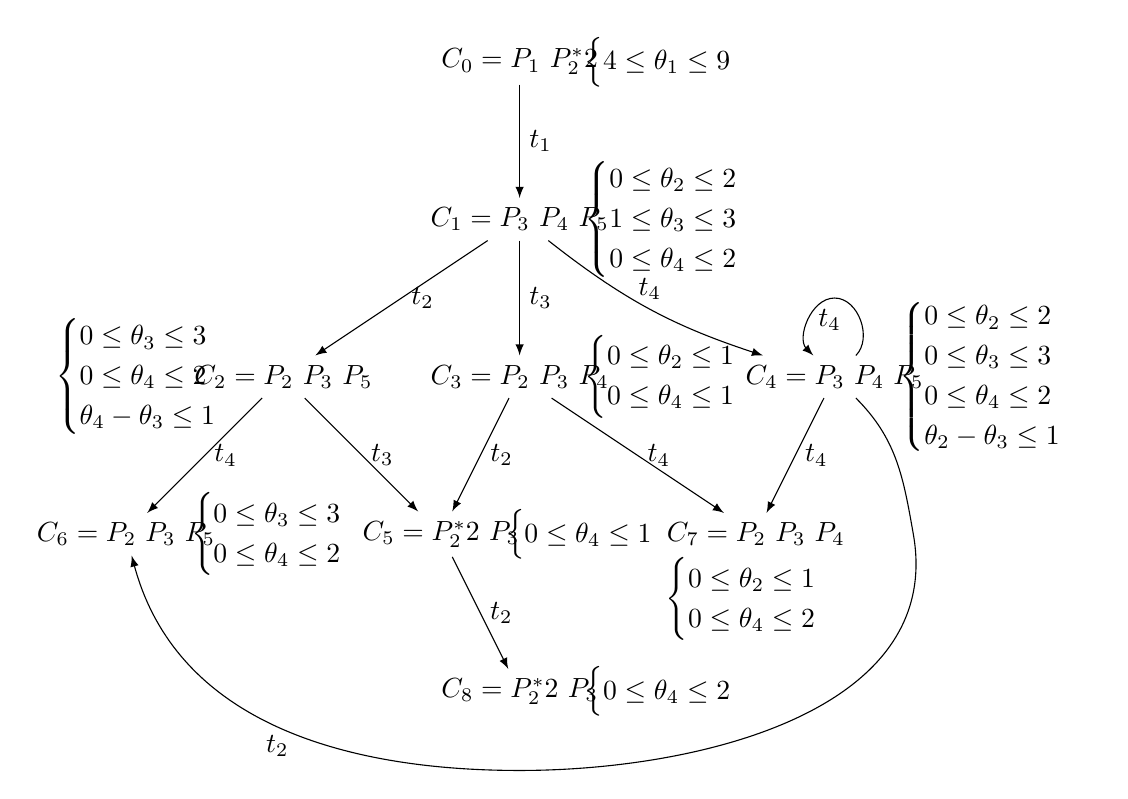
\begin{tikzpicture}
    % Liste des Marquages des classes
    \node (M0) at (0,8) {$C_0 = P_1\ P_2^*2$};
    \draw (0,8) node[right = 20pt] {$
      \begin{cases}
        4 \leq \theta_1 \leq 9
      \end{cases}
      $};
    \node (M1) at (0,6) {$C_1 = P_3\ P_4\ P_5$};
    \draw (0,6) node[right = 20pt] {$
      \begin{cases}
        0 \leq \theta_2 \leq 2\\
        1 \leq \theta_3 \leq 3\\
        0 \leq \theta_4 \leq 2
      \end{cases}
      $};
    \node (M2) at (-3,4) {$C_2 = P_2\ P_3\ P_5$};
    \draw (-3,4) node[left = 10pt] {$
      \begin{cases}
        0 \leq \theta_3 \leq 3\\
        0 \leq \theta_4 \leq 2\\
        \theta_4 - \theta_3 \leq 1
      \end{cases}
      $};
    \node (M3) at (0,4) {$C_3 = P_2\ P_3\ P_4$};
    \draw (0,4) node[right = 20pt] {$
      \begin{cases}
        0 \leq \theta_2 \leq 1\\
        0 \leq \theta_4 \leq 1
      \end{cases}
      $};
    \node (M4) at (4,4) {$C_4 = P_3\ P_4\ P_5$};
    \draw (4,4) node[right = 20pt] {$
      \begin{cases}
        0 \leq \theta_2 \leq 2\\
        0 \leq \theta_3 \leq 3\\
        0 \leq \theta_4 \leq 2\\
        \theta_2 - \theta_3 \leq 1
      \end{cases}
      $};
    \node (M5) at (-1,2) {$C_5 = P_2^*2\ P_3$};
    \draw (-1,2) node[right = 20pt] {$
      \begin{cases}
        0 \leq \theta_4 \leq 1
      \end{cases}
      $};
    \node (M6) at (-5,2) {$C_6 = P_2\ P_3\ P_5$};
    \draw (-5,2) node[right = 20pt] {$
      \begin{cases}
        0 \leq \theta_3 \leq 3\\
        0 \leq \theta_4 \leq 2
      \end{cases}
      $};
    \node (M7) at (3,2) {$C_7 = P_2\ P_3\ P_4$};
    \draw (3,2) node[below = 5pt] {$
      \begin{cases}
        0 \leq \theta_2 \leq 1\\
        0 \leq \theta_4 \leq 2
      \end{cases}
      $};
    \node (M8) at (0,0) {$C_8 = P_2^*2\ P_3$};
    \draw (0,0) node[right = 20pt] {$
      \begin{cases}
        0 \leq \theta_4 \leq 2
      \end{cases}
      $};



     % Liste des arcs
    \draw[->,>=latex] (M0) -- (M1) node[midway, right]{$t_1$};
    \draw[->,>=latex] (M1) -- (M2) node[midway, right]{$t_2$};
    \draw[->,>=latex] (M1) -- (M3) node[midway, right]{$t_3$};
    \draw[->,>=latex] (M1) to[bend right=10] node[midway, above]{$t_4$} (M4);
    \draw[->,>=latex] (M2) -- (M5) node[midway, right]{$t_3$};
    \draw[->,>=latex] (M2) -- (M6) node[midway, right]{$t_4$};
    \draw[->,>=latex] (M3) -- (M5) node[midway, right]{$t_2$};
    \draw[->,>=latex] (M3) -- (M7) node[midway, right]{$t_4$};
    \draw[->,>=latex] (M4) -- (M7) node[midway, right]{$t_4$};
    \draw[->,>=latex] (M5) -- (M8) node[midway, right]{$t_2$};
    \draw[->,>=latex] (M4) to[out=45, in=0] (4,5) to[out=180, in=135] node[midway, right]{$t_4$} (M4);
    \draw[->,>=latex] (M4) to[out=-45,in=100] (5,2)to[out=-80, in=0] (0,-1) to[out=180, in=-75] node[midway, below]{$t_2$} (M6);


  \end{tikzpicture}
  \caption{Graphe des classes} \label{fig:M10}
\end{figure}


\subsection{Question 2}

Dans ce graphe des classes nous n'avons que des composantes fortement connexe unitaire.

\begin{figure}[H]
  \centering
  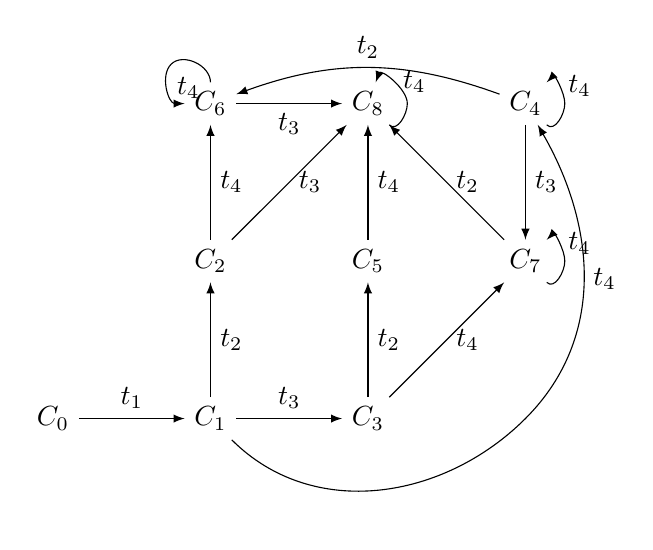
\begin{tikzpicture}
    % Liste des Marquages des classes
    \node (C0) at (0,0) {$C_0$};
    \node (C1) at (2,0) {$C_1$};
    \node (C2) at (2,2) {$C_2$};
    \node (C3) at (4,0) {$C_3$};
    \node (C4) at (6,4) {$C_4$};
    \node (C5) at (4,2) {$C_5$};
    \node (C6) at (2,4) {$C_6$};
    \node (C7) at (6,2) {$C_7$};
    \node (C8) at (4,4) {$C_8$};

 % Liste des arcs
    \draw[->,>=latex] (C0) -- (C1) node[midway, above]{$t_1$};
    \draw[->,>=latex] (C1) -- (C2) node[midway, right]{$t_2$};
    \draw[->,>=latex] (C1) -- (C3) node[midway, above]{$t_3$};
    \draw[->,>=latex] (C2) -- (C6) node[midway, right]{$t_4$};
    \draw[->,>=latex] (C2) -- (C8) node[midway, right]{$t_3$};
    \draw[->,>=latex] (C3) -- (C5) node[midway, right]{$t_2$};
    \draw[->,>=latex] (C3) -- (C7) node[midway, right]{$t_4$};
    \draw[->,>=latex] (C6) -- (C8) node[midway, below]{$t_3$};
    \draw[->,>=latex] (C5) -- (C8) node[midway, right]{$t_4$};
    \draw[->,>=latex] (C7) -- (C8) node[midway, right]{$t_2$};
    \draw[->,>=latex] (C4) -- (C7) node[midway, right]{$t_3$};
    \draw[->,>=latex] (C4) to[bend right=20] node[midway, above]{$t_2$} (C6);
    \draw[->,>=latex] (C1) to[out=-45, in=225] (6,0) to[out=45, in=-60] node[midway, right]{$t_4$}(C4);
    \draw[->,>=latex] (C6) to[out=90, in=45] (1.5,4.5) to[out=225, in=180] node[midway, right]{$t_4$}(C6);
    \draw[->,>=latex] (C8) to[out=-45, in=-90] (4.5,4) to[out=90, in=70] node[midway, right]{$t_4$}(C8);
    \draw[->,>=latex] (C4) to[out=-45, in=-90] (6.5,4) to[out=90, in=45] node[midway, right]{$t_4$}(C4);
    \draw[->,>=latex] (C7) to[out=-45, in=-90] (6.5,2) to[out=90, in=45] node[midway, right]{$t_4$}(C7);


  \end{tikzpicture}
  \caption{Graphe des composantes fortement connexes} \label{fig:M10}
\end{figure}


\end{document}
